% =====================================================================
%  PROYECTO DE GRADO — Ingeniería de Sistemas, UMSS
%  Sistema Inteligente de Entrenamiento en Gimnasios con Realidad
%  Aumentada e Inteligencia Artificial
%
%  VERSIÓN DE REVISIÓN (usa los archivos de mejorado/; los originales no se tocan)
%  Compilar:  pdflatex main  ->  pdflatex main   (o: latexmk -pdf main.tex)
%  En Overleaf: subir la carpeta completa y compilar con pdfLaTeX.
% =====================================================================
\documentclass[11pt, letterpaper, oneside]{report}

% =====================================================================
%  PAQUETES Y FORMATO GENERAL
% =====================================================================

% =====================================================================
%  Formato según la "Guía para la elaboración de trabajos de grado"
%  (Carreras de Ing. Informática e Ing. de Sistemas, FCyT-UMSS, 2013):
%   - Fuente Arial 11 (párrafos), 12 MAYÚSCULAS (títulos), 11 (subtítulos)
%   - Interlineado sencillo, espaciado posterior 6 pt, justificado, sin sangría
%   - Carta; márgenes izq. 3 cm, der. 2 cm, sup. 2 cm, inf. 2 cm
%   - Número de página en el pie, centrado
%   - Figuras y cuadros: número, descripción y fuente DEBAJO; centrados y con recuadro
% =====================================================================

% ---------- Fuente Arial ----------
% Con XeLaTeX/LuaLaTeX se usa Arial real (o TeX Gyre Heros si no está instalada).
% Con pdfLaTeX se usa Helvetica, de métricas equivalentes a Arial.
\usepackage{iftex}
\ifPDFTeX
  \usepackage[utf8]{inputenc}
  \usepackage[T1]{fontenc}
  \usepackage[scaled=1]{helvet}
  \renewcommand{\familydefault}{\sfdefault}
\else
  \usepackage{fontspec}
  \IfFontExistsTF{Arial}{\setmainfont{Arial}\setsansfont{Arial}}
                       {\setmainfont{TeX Gyre Heros}\setsansfont{TeX Gyre Heros}}
\fi
\usepackage[spanish, es-tabla, es-noshorthands, es-nodecimaldot]{babel}
\usepackage{csquotes}

% ---------- Página carta y márgenes ----------
\usepackage[letterpaper, top=2cm, bottom=2cm, left=3cm, right=2cm,
            headheight=14pt, footskip=1cm]{geometry}

% ---------- Gráficos, colores y diagramas ----------
\usepackage{graphicx}
\usepackage[table]{xcolor}
\usepackage{tikz}
\usetikzlibrary{positioning, arrows.meta, shapes.geometric, shapes.misc,
                fit, backgrounds, calc, shadows, shapes.multipart}
\usepackage{pgfgantt}

% ---------- Tablas ----------
\usepackage{array}
\usepackage{booktabs}
\usepackage{tabularx}
\usepackage{longtable}
\usepackage{needspace}
\setlength{\LTpost}{2pt}
\usepackage{multirow}
\usepackage{makecell}
\renewcommand{\arraystretch}{1.25}
% Tablas con cuadrícula: bordes en todas las celdas y encabezado sombreado
\definecolor{encabezado}{gray}{0.88}
\setlength{\arrayrulewidth}{0.5pt}
\newcolumntype{L}[1]{>{\raggedright\arraybackslash}p{#1}}
\newcolumntype{C}[1]{>{\centering\arraybackslash}p{#1}}
\newcolumntype{Y}{>{\raggedright\arraybackslash}X}

% ---------- Listas y leyendas ----------
\usepackage{enumitem}
\setlist{itemsep=2pt, topsep=4pt, parsep=0pt}
% Leyendas DEBAJO de figuras y cuadros: "Figura 2-1. Descripción. Fuente: ..."
\usepackage[font=small, labelfont=bf, labelsep=period, justification=centering,
            figureposition=bottom, tableposition=bottom, skip=6pt]{caption}
% Recuadro de las figuras
\setlength{\fboxsep}{0pt}
\setlength{\fboxrule}{0.5pt}
\usepackage{float}
\usepackage{amsmath, amssymb}

% ---------- Código fuente ----------
\usepackage{listings}
\definecolor{codegreen}{rgb}{0,0.5,0.2}
\definecolor{codegray}{rgb}{0.5,0.5,0.5}
\definecolor{codepurple}{rgb}{0.58,0,0.82}
\definecolor{backcolour}{rgb}{0.96,0.97,0.96}

\lstdefinelanguage{TypeScript}{
  keywords={abstract, any, as, async, await, boolean, break, case, catch,
    class, const, continue, default, else, enum, export, extends, false,
    finally, for, from, function, if, implements, import, in, interface,
    let, new, null, number, of, private, public, readonly, return, string,
    switch, this, throw, true, try, type, typeof, undefined, void, while},
  sensitive=true,
  comment=[l]{//},
  morecomment=[s]{/*}{*/},
  morestring=[b]",
  morestring=[b]',
  morestring=[b]`
}

\lstdefinelanguage{FirestoreRules}{
  keywords={rules_version, service, match, allow, if, function, return,
    let, read, write, create, update, delete, true, false, is, in},
  sensitive=true,
  comment=[l]{//},
  morestring=[b]'
}

\lstdefinestyle{tesis}{
  backgroundcolor=\color{backcolour},
  commentstyle=\color{codegreen}\itshape,
  keywordstyle=\color{magenta!70!black}\bfseries,
  numberstyle=\tiny\color{codegray},
  stringstyle=\color{codepurple},
  basicstyle=\ttfamily\scriptsize,
  breakatwhitespace=false,
  breaklines=true,
  captionpos=b,
  keepspaces=true,
  numbers=left,
  numbersep=6pt,
  showspaces=false,
  showstringspaces=false,
  showtabs=false,
  tabsize=2,
  frame=single,
  rulecolor=\color{black!20},
  xleftmargin=1.5em,
  framexleftmargin=1.2em,
  extendedchars=true,
  literate=
    {á}{{\'a}}1 {é}{{\'e}}1 {í}{{\'i}}1 {ó}{{\'o}}1 {ú}{{\'u}}1
    {Á}{{\'A}}1 {É}{{\'E}}1 {Í}{{\'I}}1 {Ó}{{\'O}}1 {Ú}{{\'U}}1
    {ñ}{{\~n}}1 {Ñ}{{\~N}}1 {ü}{{\"u}}1 {¿}{{?`}}1 {¡}{{!`}}1
    {→}{{$\rightarrow$}}1 {·}{{$\cdot$}}1 {…}{{...}}3
    {—}{{--}}2 {─}{{-}}1 {│}{{|}}1 {├}{{+}}1 {└}{{+}}1 {┌}{{+}}1
    {┐}{{+}}1 {┘}{{+}}1 {┬}{{+}}1 {┴}{{+}}1 {┼}{{+}}1 {┤}{{+}}1
    {̀}{{\textbackslash{}u0300}}6 {ͯ}{{\textbackslash{}u036f}}6
}
\lstset{style=tesis}
\renewcommand{\lstlistingname}{Código}
\renewcommand{\lstlistlistingname}{ÍNDICE DE CÓDIGOS FUENTE}

% ---------- Hipervínculos ----------
\usepackage[hyphens]{url}
\usepackage{hyperref}
\hypersetup{
  plainpages=false,
  pdfpagelabels=true,
  colorlinks=true,
  linkcolor=black,
  urlcolor=black,
  citecolor=black,
  filecolor=black,
  pdftitle={Sistema inteligente de entrenamiento en gimnasios},
  pdfauthor={Erika Chino Alanoca}
}

% ---------- Bibliografía (estilo autor-año, compatible con APA) ----------
\usepackage[round, authoryear]{natbib}
\setcitestyle{aysep={,}}

% ---------- Interlineado y párrafos ----------
\usepackage{setspace}
\singlespacing                   % interlineado sencillo
\setlength{\parindent}{0pt}      % sin sangría
\setlength{\parskip}{6pt}        % espaciado posterior 6 pt

% ---------- Encabezados y pies de página ----------
\usepackage{fancyhdr}
\pagestyle{fancy}
\fancyhf{}
\fancyfoot[C]{\thepage}         % número de página centrado en el pie
\renewcommand{\headrulewidth}{0pt}
\fancypagestyle{plain}{\fancyhf{}\fancyfoot[C]{\thepage}\renewcommand{\headrulewidth}{0pt}}

% ---------- Numeración: capítulos en romanos, secciones en arábigos ----------
\renewcommand{\thechapter}{\Roman{chapter}}
\renewcommand{\thesection}{\arabic{chapter}.\arabic{section}}
\renewcommand{\thefigure}{\arabic{chapter}-\arabic{figure}}
\renewcommand{\thetable}{\arabic{chapter}-\arabic{table}}
\AtBeginDocument{\renewcommand{\thelstlisting}{\arabic{chapter}-\arabic{lstlisting}}}
\renewcommand{\theequation}{\arabic{chapter}.\arabic{equation}}
\setcounter{secnumdepth}{3}
\setcounter{tocdepth}{2}

% ---------- Títulos y subtítulos ----------
% Títulos (capítulos): 12 pt, negrilla, MAYÚSCULAS, centrados, 6 pt antes y después.
% Subtítulos: 11 pt, negrilla, alineados a la izquierda, 6 pt antes y después.
\usepackage{titlesec}
\newcommand{\fuentetitulo}{\fontsize{12}{14}\selectfont}
\titleformat{\chapter}[block]
  {\normalfont\fuentetitulo\bfseries\centering}
  {\MakeUppercase{\chaptertitlename}\ \thechapter:\ }
  {0pt}
  {\MakeUppercase}
\titlespacing*{\chapter}{0pt}{0pt}{6pt}
\titleformat{\section}{\normalfont\normalsize\bfseries}{\thesection.}{0.5em}{}
\titleformat{\subsection}{\normalfont\normalsize\bfseries}{\thesubsection.}{0.5em}{}
\titleformat{\subsubsection}{\normalfont\normalsize\bfseries}{\thesubsubsection.}{0.5em}{}
\titlespacing*{\section}{0pt}{6pt}{0pt}
\titlespacing*{\subsection}{0pt}{6pt}{0pt}
\titlespacing*{\subsubsection}{0pt}{6pt}{0pt}
\titlespacing*{\paragraph}{0pt}{6pt}{0.5em}

% ---------- Nombres en español ----------
\addto\captionsspanish{%
  \renewcommand{\contentsname}{ÍNDICE GENERAL}%
  \renewcommand{\listfigurename}{ÍNDICE DE FIGURAS}%
  \renewcommand{\listtablename}{ÍNDICE DE TABLAS}%
  \renewcommand{\appendixname}{Anexo}%
  \renewcommand{\chaptername}{Capítulo}%
}
% En los anexos la etiqueta es "ANEXO A -- ..."
\usepackage{etoolbox}
\appto\appendix{%
  \renewcommand{\thechapter}{\Alph{chapter}}%
  \renewcommand{\thesection}{\Alph{chapter}.\arabic{section}}%
  \renewcommand{\thefigure}{\Alph{chapter}-\arabic{figure}}%
  \renewcommand{\thetable}{\Alph{chapter}-\arabic{table}}%
  \renewcommand{\thelstlisting}{\Alph{chapter}.\arabic{lstlisting}}%
}

% ---------- Ancho de números en los índices ----------
\usepackage{tocloft}
\renewcommand{\cftchapfont}{\bfseries}
\renewcommand{\cftchappagefont}{\bfseries}
\setlength{\cftchapnumwidth}{2.6em}
\setlength{\cftsecnumwidth}{2.6em}
\setlength{\cftsubsecnumwidth}{3.4em}
\setlength{\cftfignumwidth}{2.8em}
\setlength{\cfttabnumwidth}{2.8em}
% Títulos de los índices: 12 pt, negrilla, centrados, sin salto de página propio
\renewcommand{\cfttoctitlefont}{\hfill\fuentetitulo\bfseries}
\renewcommand{\cftaftertoctitle}{\hfill}
\renewcommand{\cftloftitlefont}{\hfill\fuentetitulo\bfseries}
\renewcommand{\cftafterloftitle}{\hfill}
\renewcommand{\cftlottitlefont}{\hfill\fuentetitulo\bfseries}
\renewcommand{\cftafterlottitle}{\hfill}
\setlength{\cftbeforetoctitleskip}{0pt}
\setlength{\cftaftertoctitleskip}{6pt}
\setlength{\cftbeforeloftitleskip}{12pt}
\setlength{\cftafterloftitleskip}{6pt}
\setlength{\cftbeforelottitleskip}{12pt}
\setlength{\cftafterlottitleskip}{6pt}
\setlength{\cftbeforechapskip}{4pt}
\setlength{\emergencystretch}{2em}

% =====================================================================
%  VARIABLES GLOBALES DEL PROYECTO DE GRADO
%  (cambiar aquí y se actualiza en todo el documento)
% =====================================================================

% Datos institucionales
\newcommand{\universidad}{UNIVERSIDAD MAYOR DE SAN SIMÓN}
\newcommand{\facultad}{FACULTAD DE CIENCIAS Y TECNOLOGÍA}
\newcommand{\carrera}{CARRERA DE INGENIERÍA DE SISTEMAS}
\newcommand{\ubicacion}{Cochabamba -- Bolivia}
\newcommand{\fechaDefensa}{2026}  % TODO: mes-año de la defensa, p. ej. 11-2026

% Datos del proyecto
\newcommand{\tituloTesis}{SISTEMA INTELIGENTE DE ENTRENAMIENTO EN GIMNASIOS CON REALIDAD AUMENTADA E INTELIGENCIA ARTIFICIAL}
\newcommand{\modalidadTesis}{Proyecto de Grado presentado para optar al Diploma Académico de Licenciatura en Ingeniería de Sistemas}
\newcommand{\nombreApp}{CoachApp}

% Personas
\newcommand{\autorTesis}{Erika Chino Alanoca}
\newcommand{\tutorTesis}{Mgr. Jimmy Villarroel Novillo}
\newcommand{\docenteTesis}{MSc. Américo Fiorilo Lozada}

% =====================================================================
%  COMANDOS PROPIOS
% =====================================================================

% Nombre de archivo, ruta o identificador de código dentro del texto
\newcommand{\archivo}[1]{\texttt{\small #1}}

% Marca visible para lo que la autora debe completar antes de imprimir.
% Para ocultar todas las marcas: \renewcommand{\pendiente}[1]{}
\newcommand{\pendiente}[1]{\textcolor{red!70!black}{\textbf{[PENDIENTE:} #1\textbf{]}}}

% Captura de pantalla de la app.
%   \captura{archivo-sin-extension}{Leyenda}{etiqueta}
% Coloca las capturas en figuras/capturas/ (png o jpg). Mientras el archivo
% no exista, se dibuja un recuadro con el nombre esperado.
\newcommand{\captura}[3]{%
  \begin{figure}[H]
    \centering
    \IfFileExists{figuras/capturas/#1.png}{%
      \includegraphics[height=0.42\textheight]{figuras/capturas/#1.png}}{%
    \IfFileExists{figuras/capturas/#1.jpg}{%
      \includegraphics[height=0.42\textheight]{figuras/capturas/#1.jpg}}{%
      \fbox{\parbox[c][0.30\textheight][c]{0.32\textwidth}{\centering\small
        Captura de pantalla\\[4pt]\texttt{\scriptsize figuras/capturas/}\\\texttt{\scriptsize\detokenize{#1}.png}}}}}
    \caption{#2}
    \label{#3}
    \fuente{Elaboración propia.}
  \end{figure}}

% Dos capturas lado a lado
%   \capturados{archivo1}{subleyenda1}{archivo2}{subleyenda2}{Leyenda}{etiqueta}
\newcommand{\imagencaptura}[1]{%
  \IfFileExists{figuras/capturas/#1.png}{%
    \includegraphics[height=0.36\textheight]{figuras/capturas/#1.png}}{%
  \IfFileExists{figuras/capturas/#1.jpg}{%
    \includegraphics[height=0.36\textheight]{figuras/capturas/#1.jpg}}{%
    \fbox{\parbox[c][0.28\textheight][c]{0.44\textwidth}{\centering\small
      Captura de pantalla\\[4pt]\texttt{\scriptsize figuras/capturas/}\\\texttt{\scriptsize\detokenize{#1}.png}}}}}}
\newcommand{\capturados}[6]{%
  \begin{figure}[H]
    \centering
    \begin{minipage}[t]{0.47\textwidth}\centering
      \imagencaptura{#1}\\[2pt]{\small (a) #2}
    \end{minipage}\hfill
    \begin{minipage}[t]{0.47\textwidth}\centering
      \imagencaptura{#3}\\[2pt]{\small (b) #4}
    \end{minipage}
    \caption{#5}
    \label{#6}
    \fuente{Elaboración propia.}
  \end{figure}}

% Nota de fuente al pie de tablas y figuras
\newcommand{\fuente}[1]{\par\vspace{2pt}{\footnotesize\textit{Fuente:} #1}}

% Estilos TikZ comunes para diagramas
\tikzset{
  caja/.style={rectangle, rounded corners=3pt, draw=black!70, fill=white,
               minimum height=0.9cm, align=center, font=\small, inner sep=5pt},
  capa/.style={rectangle, draw=black!60, fill=#1, minimum width=13.5cm,
               minimum height=1.6cm, align=left, font=\small},
  capa/.default={black!5},
  flecha/.style={-{Stealth[length=2.5mm]}, thick, black!70},
  flechad/.style={-{Stealth[length=2.5mm]}, thick, dashed, black!60},
  casouso/.style={ellipse, draw=black!70, fill=green!4, minimum width=3.6cm,
                  minimum height=0.85cm, align=center, font=\footnotesize, inner sep=1pt},
  entidad/.style={rectangle, draw=black!70, fill=white, align=left,
                  font=\scriptsize\ttfamily, inner sep=4pt, rectangle split,
                  rectangle split parts=2, rectangle split part fill={green!12,white}},
}

% Actor UML (monigote) — \actor{nombre-nodo}{posición}{etiqueta}
\newcommand{\actor}[3]{%
  \begin{scope}[shift={#2}]
    \draw[thick] (0,0.55) circle (0.18);
    \draw[thick] (0,0.37) -- (0,-0.15);
    \draw[thick] (-0.3,0.2) -- (0.3,0.2);
    \draw[thick] (0,-0.15) -- (-0.25,-0.55);
    \draw[thick] (0,-0.15) -- (0.25,-0.55);
    \node[font=\small, below] at (0,-0.6) {#3};
    \coordinate (#1) at (0.35,0.1);
  \end{scope}}

% Lista con viñetas dentro de una celda de tabla (columnas p{} / X)
\newenvironment{tablista}
  {\begin{itemize}[leftmargin=1.1em, nosep, topsep=0pt, partopsep=0pt,
     before={\vspace{-0.55\baselineskip}}, after={\vspace{-\baselineskip}}]}
  {\end{itemize}}

% Párrafo de "Conclusión:" debajo de las tablas comparativas
\newcommand{\conclusion}[1]{\par\textbf{Conclusión:} #1\par}

% Encabezado en negrita dentro de una sección (sin numerar)
\newcommand{\titulillo}[1]{\par\medskip\noindent\textbf{#1}\par}

% Lista de referencias con sangría francesa (formato APA)
\newenvironment{referenciasapa}
  {\begin{list}{}{\setlength{\leftmargin}{1.27cm}\setlength{\itemindent}{-1.27cm}
     \setlength{\itemsep}{6pt}\setlength{\parsep}{0pt}}\raggedright}
  {\end{list}}


\begin{document}

% ---------------- Páginas preliminares ----------------
\hypersetup{pageanchor=false}
\begin{titlepage}
    \centering

    % Encabezado con los dos logos
    \begin{minipage}[c]{0.18\textwidth}
        
\includegraphics[width=\textwidth]{figuras/logo_umss.png}
    \end{minipage}%
    \begin{minipage}[c]{0.64\textwidth}
        \centering
        {\bfseries \small \universidad \par}
        \vspace{0.1cm}
        {\bfseries \small \facultad \par}
        \vspace{0.1cm}
        {\bfseries \small \carrera \par}
    \end{minipage}%
    \begin{minipage}[c]{0.18\textwidth}
        
\includegraphics[width=\textwidth]{figuras/logo_fcyt.jpg}
    \end{minipage}

    \vspace{3cm}

    % Cuadro del título
    \setlength{\fboxrule}{1.5pt}
    \setlength{\fboxsep}{14pt}
    \fbox{%
        \begin{minipage}{0.85\textwidth}
            \centering
            \bfseries \large \tituloTesis
        \end{minipage}%
    }

    \vspace{2.5cm}

    \begin{minipage}{0.8\textwidth}
        \centering
        \small \modalidadTesis
    \end{minipage}

    \vspace{3cm}

    % Datos de la autora, tutor y docente
    \begin{raggedright}
        \hspace{0.05\textwidth}
        \begin{tabular}{ll}
            \textbf{Presentado por:} & \autorTesis \\[0.2cm]
            \textbf{Tutor:}          & \tutorTesis
        \end{tabular}
    \end{raggedright}

    \vfill

    {\bfseries \small \ubicacion \par}
    \vspace{0.1cm}
    {\bfseries \small \fechaDefensa \par}
\end{titlepage}

\hypersetup{pageanchor=true}

\pagenumbering{roman}
\clearpage
\thispagestyle{plain}

\vspace*{0.48\textheight}

{\fontfamily{ptm}\selectfont\bfseries\itshape
\noindent Dedicatoria\par
\vspace{1.2em}
\noindent A mis padres Federico Chino Salinas y Silvia Alanoca Gutierrez, quienes siempre me apoyaron y me brindaron su amor incondicional, gracias por enseñarme que con esfuerzo y dedicación se pueden alcanzar los sueños.\par
\vspace{1.2em}
\noindent A mis hermanas, mi mejor amiga y a toda mi familia por su apoyo constante, por haber confiado en mí y en mis capacidades, ahora cumplo uno de mis sueños y agradezco a todos los que, de una u otra manera, fueron parte de este camino.
}

\vfill

\clearpage

\thispagestyle{plain}

\begin{center}

    {\Large \bfseries AGRADECIMIENTOS}

\end{center}

\vspace{0.8cm}

Doy gracias a Dios por darme la vida, la salud y la sabiduría para llegar hasta este momento y permitirme cumplir una de las metas más importantes de mi vida.

A mi familia, gracias por su apoyo, por creer en mí y por acompañarme durante todo este camino. Muchas veces fueron mi motivación para seguir adelante, incluso cuando las cosas no fueron fáciles.

Agradezco a la Universidad Mayor de San Simón y a la Facultad de Ciencias y Tecnología por haber sido parte fundamental de mi formación y por brindarme las herramientas y conocimientos que me permitieron crecer tanto profesional como personalmente.

A mi tutor, Lic. Jimmy Villarroel Novillo, gracias por su paciencia, orientación y por compartir sus conocimientos durante el desarrollo de este proyecto.

Finalmente, gracias a mis amigos por acompañarme durante estos años, por los buenos momentos, las experiencias y todos los recuerdos que me llevo de esta etapa.

Gracias a todos los que, de una u otra manera, fueron parte de este camino.

\vfill

% =====================================================================
%  FICHA RESUMEN (versión mejorada) — debe caber en UNA sola página.
%  Cambios respecto al original: describe los seis capítulos vigentes,
%  incluye los resultados verificados (ml/results) y las limitaciones.
% =====================================================================
\clearpage
\thispagestyle{plain}

\begin{center}
    {\Large \bfseries FICHA RESUMEN}
\end{center}

\vspace{0.2cm}

\begin{tabular}{@{}ll}
\textbf{Grado:} & Licenciatura en Ingeniería de Sistemas \\
\textbf{Modalidad:} & Proyecto de Grado \\
\textbf{Facultad:} & Ciencias y Tecnología \\
\textbf{Carrera:} & Ingeniería de Sistemas \\
\textbf{Título del trabajo:} & \parbox[t]{10cm}{Sistema Inteligente de Entrenamiento en
Gimnasios con Realidad Aumentada e Inteligencia Artificial} \\
\textbf{Autora:} & \autorTesis \\
\textbf{Tutor:} & \tutorTesis \\
\end{tabular}

\vspace{0.3cm}
\small

En el primer capítulo se analiza el abandono temprano de los usuarios de
gimnasios, asociado a la falta de orientación, motivación y seguimiento
personalizado, y se formulan el problema, los objetivos y el alcance de un
sistema de entrenamiento para Android.

En el segundo capítulo se desarrolla el marco teórico: metodologías de
desarrollo de software tradicionales y ágiles (se justifica Mobile-D),
programación móvil, realidad aumentada, inteligencia artificial, fundamentos
del entrenamiento físico y tecnologías de desarrollo.

En el tercer capítulo se describe el área de aplicación, la adopción de la
metodología Mobile-D (exploración, inicialización, producción, estabilización
y pruebas), los roles y las técnicas de recolección de información.

En el cuarto capítulo se documenta el desarrollo de la aplicación CoachApp con
React Native, Expo y TypeScript sobre Firebase (autenticación, base de datos,
almacenamiento, Cloud Functions y App Check), con arquitectura
cliente--servidor en capas Modelo--Vista--Controlador. El sistema incluye un
catálogo de 35 tipos de máquinas, un generador de rutinas basado en reglas con
un recomendador de TensorFlow Lite, un reconocedor de máquinas por imagen
(MobileNetV2) con un escáner que superpone la ficha de la máquina sobre la
cámara, el registro de peso, IMC y alimentación, y reportes de progreso.

En el quinto capítulo se presentan y discuten los resultados: el reconocedor
acierta la máquina en el 38,5\,\% de las fotos (61,4\,\% entre las tres primeras
sugerencias) en un escenario de campo simulado, por lo que el usuario siempre
confirma el resultado; el recomendador reproduce las reglas con una exactitud
del 99,8\,\% sobre datos sintéticos, lo que mide su fidelidad y no la calidad de
las rutinas. Se declaran las limitaciones: la superposición de la cámara no
tiene registro tridimensional y la validación con usuarios y con fotografías de
gimnasios reales queda pendiente.

En el sexto capítulo se presentan las conclusiones por objetivo y las
recomendaciones para trabajos futuros. El sistema no reemplaza la supervisión
de entrenadores ni de nutricionistas.
\normalsize


% Índice de contenido, de cuadros y de figuras en una sola hoja (guía, punto 4)
\clearpage
\tableofcontents
\listoftables
\listoffigures
\clearpage

% ---------------- Cuerpo ----------------
\pagenumbering{arabic}

\chapter{INTRODUCCIÓN}
\label{cap:introduccion}

En la actualidad, la práctica del ejercicio físico en gimnasios ha cobrado gran
relevancia como parte de un estilo de vida saludable. Sin embargo, diversos
estudios han evidenciado que una gran parte de los usuarios abandonan sus
rutinas en los primeros meses, principalmente por la falta de orientación,
motivación y seguimiento personalizado (Gjestvang, 2020). Esta problemática
afecta especialmente a los principiantes, quienes enfrentan barreras como el
desconocimiento del uso correcto de las máquinas, el alto coste de entrenadores
personales y la ausencia de planificación estructurada.

En respuesta a esta necesidad, se han desarrollado diversas soluciones
tecnológicas que buscan mejorar la experiencia del usuario en el gimnasio, como
aplicaciones móviles con realidad aumentada (Cruz, 2024) y sistemas de
información para rutinas y dietas (Fernández, 2018). No obstante, muchas de
estas herramientas carecen de personalización profunda y seguimiento
inteligente.

Este proyecto propone el desarrollo de una aplicación móvil basada en realidad
aumentada e inteligencia artificial, orientada a guiar a los usuarios en el uso
correcto de máquinas de ejercicio, planificar rutinas personalizadas y realizar
un seguimiento del progreso físico. La solución busca democratizar el acceso a
la orientación profesional, reducir el abandono temprano y fomentar la
constancia en el entrenamiento físico, utilizando tecnologías modernas como
React Native, Firebase y TensorFlow Lite.

Con esto, se pretende contribuir no solo al bienestar individual, sino también
a la optimización de recursos en gimnasios, ofreciendo una herramienta
accesible, interactiva y eficaz para la autogestión del entrenamiento.

% =====================================================================
\section{Antecedentes}
\label{sec:antecedentes}

(Yépez, 2017) en su proyecto de grado cuyo objetivo principal es la creación de
un gimnasio que combine asesoramiento presencial y virtual, orientado a la nueva
disciplina llamada Street Workout, que consiste en utilizar el propio peso
corporal para ejercitarse.

(Gjestvang, 2020) se realizó un estudio longitudinal en Noruega con el objetivo
de identificar las principales barreras en la iniciación y adherencia al
ejercicio en gimnasios. El proyecto evidenció que entre el 40\,\% y el 65\,\% de
los nuevos usuarios abandonan la asistencia regular en los primeros meses,
principalmente por la falta de motivación, orientación adecuada y seguimiento
personalizado. Estos resultados destacan la importancia de diseñar
herramientas tecnológicas que fortalezcan la adherencia a programas de
ejercicio estructurados.

(Cruz, 2024) desarrolló un proyecto de grado desarrollado en la Universidad
Mayor de San Simón, una aplicación móvil para gimnasios que utiliza escaneo de
código QR con realidad aumentada para mejorar la experiencia de los usuarios y
la gestión de entrenamientos, que permite a los usuarios obtener instrucciones
detalladas en tiempo real sobre los ejercicios.

(Fernandez, 2018) en su proyecto de grado desarrolló un sistema de información
cuyo objetivo principal es brindar apoyo a los usuarios o clientes de los
gimnasios, proporcionándoles rutinas de ejercicios y dietas, para que sirva de
guía sobre cómo usar las máquinas y como administrar sus alimentos para obtener
el objetivo deseado.

(BodBot IA Entrenador Personal, 2016) es una plataforma de fitness avanzada
creada por Edward Laux, Jason Storm y Sergio Prado, que ofrece entrenamientos de
IA personalizados según los objetivos, equipos, capacidades físicas y
dificultad del usuario, esta plataforma proporciona una guía paso a paso para
cada ejercicio, contiene personalización de peso corporal y registro de
alimentación diario.

(Ejercicios en el Gimnasio, 2021) desarrollada por Leap Fitness Group, es una
plataforma fitness para principiantes y asiduos al gimnasio, que funciona como
un entrenador personalizado, creando rutinas, mostrando la postura correcta para
realizar ejercicios esto por medio de instrucciones visuales y literales
explícitas, siguiendo el progreso con estadísticas y gráficos claros.

% =====================================================================
\section{Análisis del problema}
\label{sec:problema}

\subsection{Descripción del problema}

Este proyecto surge para resolver las principales barreras que los usuarios de
gimnasios enfrentan, particularmente la falta de orientación adecuada y la falta
de estructura en sus entrenamientos. (Gjestvang, 2020) Estudios demuestran que
entre el 40\,\% y el 65\,\% de los nuevos usuarios abandonan el gimnasio en los
primeros meses, principalmente por la falta de guía y seguimiento
personalizado. Los principales problemas identificados incluyen:

\begin{itemize}
    \item \textbf{Falta de conocimiento sobre el uso adecuado de las máquinas y
    la postura correcta:} Esto lleva a errores que pueden causar lesiones y
    dificultar el progreso hacia los objetivos físicos.
    \item \textbf{Costo elevado de los entrenadores personales:} Muchas personas
    no pueden acceder a una guía profesional debido al costo asociado, lo cual
    deja a la mayoría sin un apoyo adecuado.
    \item \textbf{Falta de seguimiento del progreso:} La falta de un sistema para
    registrar y analizar el progreso personal desmotiva a los usuarios, ya que
    no tienen una forma clara de visualizar sus avances.
    \item \textbf{Carencia de planificación estructurada del entrenamiento:} Sin
    una rutina clara y bien planificada, muchos usuarios se sienten perdidos y no
    logran aprovechar el tiempo de entrenamiento, lo cual fomenta la
    desmotivación y el abandono.
\end{itemize}

\subsection{Definición del problema}

¿Cómo desarrollar una aplicación para gimnasios que ofrezca seguimiento rutinas
de ejercicio personalizadas con Inteligencia artificial?

% =====================================================================
\section{Objetivos}
\label{sec:objetivos}

\subsection{Objetivo general}

Desarrollar un sistema inteligente para el entrenamiento en gimnasios,
proporcionando una guía estructurada y seguimiento personalizado de los
ejercicios.

\subsection{Objetivos específicos}

\begin{itemize}
    \item Guiar sobre el uso correcto de máquinas.
    \item Instruir en la ejecución correcta de ejercicios específicos.
    \item Diseñar rutinas de entrenamiento personalizadas y estructuradas,
    adaptadas a los objetivos de cada usuario.
    \item Construir herramientas de planificación que permitan a los usuarios
    organizar sus entrenamientos de manera eficiente.
    \item Registrar la ingesta de alimentos con el fin de controlar y evaluar las
    calorías consumidas por el usuario.
    \item Implementar un sistema de seguimiento del progreso físico.
    \item Generar reportes personalizados de progreso físico.
\end{itemize}

% =====================================================================
\section{Área de conocimiento}
\label{sec:area}

\textbf{Área:} Programación Móvil

\textbf{Subárea:} Sistema de Información

% =====================================================================
\section{Alcance}
\label{sec:alcance}

\begin{itemize}
    \item El sistema funcionará en sistemas operativos Android.
    \item Interfaz intuitiva para el registro de usuarios.
    \item Guía sobre el uso correcto de máquinas de gimnasio.
    \item Registrar el progreso físico (peso, estatura, edad, masa corporal).
    \item Creación de rutinas personalizadas según los objetivos del usuario.
    \item El registro de alimentación se limitará solo al conteo calórico, es
    decir una calculadora de IMC.
    \item El sistema no reemplaza la supervisión profesional de entrenadores o
    nutricionistas.
    \item No se contempla la integración con dispositivos externos (smartwatch,
    banda de frecuencia cardíaca, entre otros).
    \item El sistema funcionará con conexión a internet.
    \item La aplicación será para dispositivos móviles Android.
    \item El sistema estará disponible únicamente en idioma español.
    \item La aplicación requerirá permisos de acceso a la cámara y almacenamiento del dispositivo para el registro de progresos y la visualización de ejercicios.
\end{itemize}

% =====================================================================
\section{Justificación}
\label{sec:justificacion}

\subsection{Justificación técnica}

El proyecto es técnicamente viable gracias a la combinación de tecnologías
modernas y flexibles. Se empleará React Native con Expo para garantizar una
experiencia fluida en dispositivos Android, permitiendo un desarrollo
multiplataforma con una sola base de código.

La base de datos y autenticación estarán gestionadas por Firebase, lo que
asegura escalabilidad, sincronización en tiempo real y seguridad en el manejo de
datos de usuarios.

El componente de inteligencia artificial se implementará para generar rutinas
personalizadas, basándose en parámetros como peso, altura, edad, nivel de
experiencia y objetivos físicos. Este módulo podrá entrenarse mediante modelos
preexistentes o redes neuronales ligeras optimizadas para dispositivos móviles.

Además, se integrará un sistema de visualización interactiva con imágenes o
animaciones que muestran la postura correcta en cada ejercicio, lo cual aumenta
la comprensión y reduce el riesgo de lesiones.

En conjunto, estas tecnologías garantizan un sistema robusto, escalable y con
potencial de expansión futura.

\subsection{Justificación económica}

La aplicación representa una alternativa de bajo costo frente a los servicios
tradicionales de entrenamiento personalizado. Al automatizar la generación de
rutinas mediante inteligencia artificial, se reducen los costos asociados a la
contratación de entrenadores físicos, permitiendo que los usuarios obtengan
orientación profesional sin incurrir en gastos adicionales.

Para los gimnasios, la herramienta puede convertirse en un complemento
estratégico que optimice el tiempo de los entrenadores y mejore la retención de
clientes, al ofrecerles una plataforma moderna de autogestión del
entrenamiento. Asimismo, el desarrollo de esta aplicación se apoya en
tecnologías de código abierto (React Native, Firebase, TensorFlow Lite, etc.),
lo que disminuye considerablemente los costos de desarrollo y mantenimiento del
sistema.

\subsection{Justificación social}

Este proyecto busca eliminar las barreras que limitan la práctica constante del
ejercicio físico, ofreciendo orientación y motivación a través de la tecnología.
Está dirigido principalmente a usuarios principiantes o personas que no tienen
acceso a un entrenador personal. Contribuye a la promoción de un estilo de vida
saludable, fomenta la constancia y previene lesiones al enseñar el uso correcto
de las máquinas.

% =====================================================================
%  CAPÍTULO 2 (versión actualizada). Cambios respecto al original:
%   - Citas de autores corporativos alineadas con la bibliografía APA 7.
%   - Mobile-D: adaptación declarada (equipos pequeños, proyectos breves) y
%     días de planificación/trabajo/entrega (Abrahamsson et al., 2004).
%   - Realidad aumentada: atribución corregida y subsección de alcance.
%   - IA: modelos ligeros (Sandler et al., 2018) y antecedente de Silva Amado.
%   - Entrenamiento y nutrición: prescripción (Kraemer y Ratamess, 2004),
%     IMC/OMS y gasto energético (Mifflin et al., 1990).
%   - Afirmaciones absolutas atenuadas («garantizan», «demuestra»).
% =====================================================================
\chapter{MARCO TEÓRICO}
\label{cap:marco}

% =====================================================================
\section{Metodología de Desarrollo}
\label{sec:metodologia-desarrollo}

Una metodología de desarrollo de software es un marco de trabajo que se usa
para estructurar, planificar y controlar el proceso de desarrollo de sistemas de
información (Gabriel Maide \& Pacienzia, 2020). Asimismo el objetivo de las
distintas metodologías es el intentar organizar los equipos de trabajo para que
estos desarrollen las funciones de un programa de la mejor manera posible
(Santander Open Academy, 2020). Una metodología establece un conjunto de prácticas, técnicas
y procesos que permiten mejorar la eficiencia del trabajo, garantizar la
calidad y reducir la incertidumbre durante el ciclo de vida del software
(Pressman, 2010).

Las metodologías de desarrollo proporcionan lineamientos que facilitan la
coordinación del equipo, la definición clara de los requerimientos, la gestión
de riesgos y la evaluación del avance del proyecto. El uso de la metodología
adecuada contribuye a la minimización de riesgos, estandarización de
procedimientos y mejorar la productividad.

Las metodologías de desarrollo de software son enfoques que proporcionan un
marco claro para planificar, ejecutar y entregar proyectos de software, estas
pueden ser lineales o iterativas, se ajustan a diferentes tipos de proyectos y
equipos de acuerdo a las necesidades específicas de cada proyecto o equipo
(Abstracta Team, 2024).

% =====================================================================
\section{Metodologías de desarrollo de software tradicionales vs ágiles}
\label{sec:tradicionales-agiles}

Las metodologías de desarrollo de software se agrupan principalmente en
tradicionales y ágiles, cada una con enfoques y características distintas.

\subsection{Metodologías tradicionales}

Las metodologías tradicionales, conocidas también como predictivas, son
enfoques secuenciales y lineales, basados en una planificación detallada y
estructurada, donde cada fase debe completarse antes de iniciar la siguiente,
tampoco se puede volver hacia atrás una vez se ha cambiado de fase. Estas
metodologías, no se adaptan nada bien a los cambios, y el mundo actual cambia
constantemente (Santander Open Academy, 2020).

Este enfoque es ideal para proyectos en los que los requerimientos están bien
definidos desde el principio.

La comparación detallada de las metodologías Waterfall, Espiral, Incremental, Prototipado y Diseño rápido de aplicaciones (RAD), con su descripción y características, se presenta en la Tabla~\ref{tab:metodologias-tradicionales} del Anexo~\ref{anx:comparativas}.

\subsection{Metodologías ágiles para móvil}

Las metodologías ágiles aplicadas al desarrollo móvil surgen como respuesta a
la necesidad de adaptarse a un entorno cambiante y a ciclos de producción
rápidos. Estas metodologías están centradas en la entrega continua de valor, la
colaboración constante con el cliente y la capacidad de adaptarse a nuevos
requerimientos.

Las metodologías ágiles son las más utilizadas en la actualidad debido a su alta
flexibilidad y agilidad (Santander Open Academy, 2020). Se basan en la metodología
incremental, en la que en cada ciclo de desarrollo se agregan nuevas
funcionalidades a la aplicación final.

La comparación de las metodologías Scrum, Extreme Programming (XP), Mobile-D y Kanban, con su descripción y características, se presenta en la Tabla~\ref{tab:metodologias-agiles} del Anexo~\ref{anx:comparativas}.

% =====================================================================
\section{Mobile-D}
\label{sec:mobile-d}

La metodología Mobile-D es un enfoque ágil diseñado para el desarrollo de
software en dispositivos móviles. Surgió como resultado de investigaciones
realizadas por el VTT, con el objetivo de responder a los desafíos propios del
entorno móvil, como ciclos de producción acelerados, restricciones de hardware,
diversidad de plataformas y cambios frecuentes en los requisitos (Abrahamsson
et al., 2004).

Mobile-D es adecuada para proyectos que requieren rapidez, flexibilidad y alta
calidad. Está pensada para equipos pequeños y para proyectos de corta duración
(el artículo original menciona entregas en menos de diez semanas;
Abrahamsson et~al., 2004), por lo que su aplicación a este proyecto, individual
y de mayor duración, constituye una adaptación. La metodología combina prácticas
de diversas metodologías ágiles y de ingeniería de software.
% VERIFICAR: citar en el texto base de Mobile-D qué metodologías integra.

\subsection{Fases y etapas}

El desarrollo mediante el enfoque de Mobile-D se compone de 5 fases como se
muestra en la Figura~\ref{fig:mobile-d}, estas fases son: Exploración,
Inicialización, Producción, Estabilización y Pruebas del sistema. En cada
iteración, el método organiza el trabajo en días de planificación, de trabajo y
de entrega (Abrahamsson et~al., 2004).

\begin{figure}[H]
    \centering
    \fbox{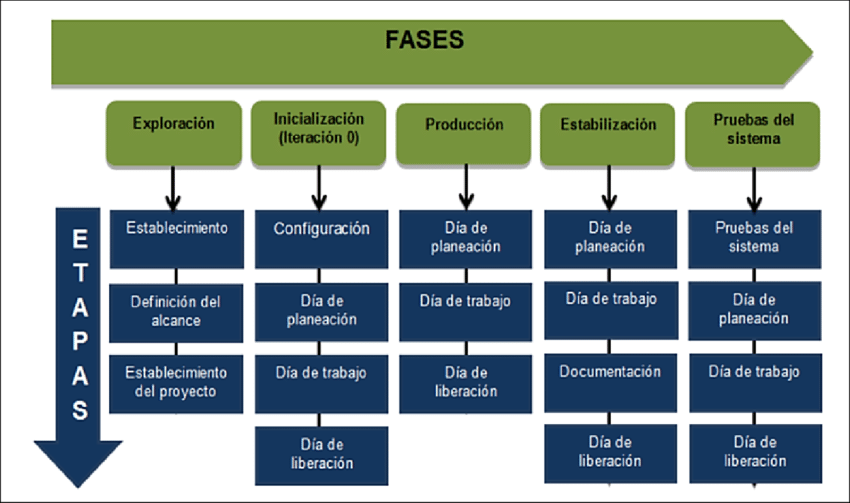
\includegraphics[width=0.68\textwidth]{figuras/docx/mobile-d-fases.png}}
    \caption{Fases y etapas de la metodología Mobile-D}
    \label{fig:mobile-d}
    \fuente{Leyva et~al. (2016).}
\end{figure}

\begin{itemize}
    \item \textbf{Fase de Exploración}

    Esta es la fase inicial donde se define el proyecto y se establecen las
    bases técnicas y organizativas. En esta fase se definen los objetivos, el
    alcance, los actores involucrados y las restricciones técnicas y
    funcionales del proyecto. También se seleccionan las tecnologías
    principales y se configura el entorno de trabajo.

    \item \textbf{Fase de Inicialización}

    En esta fase se prepara el equipo, las herramientas y la arquitectura
    técnica para comenzar las iteraciones de desarrollo. Dentro de esta fase se
    verifican los recursos humanos, tecnológicos y físicos que se necesitarán.
    Esta fase se divide en cuatro etapas: la puesta en marcha del proyecto, la
    planificación inicial, el día de prueba y día de salida (Gómez \&
    Hernández, 2016).

    \item \textbf{Fase de Producción}

    Esta fase se caracteriza por el uso de ciclos cortos e incrementales. En
    esta etapa se implementan funcionalidades mediante prácticas de desarrollo
    guiado en pruebas TDD, la integración continua y el desarrollo iterativo.
    Su objetivo principal es construir versiones funcionales del producto de
    manera progresiva, garantizando la calidad y retroalimentación constante
    durante todo el proceso.

    \item \textbf{Fase de Estabilización}

    En esta fase se integran los componentes generados durante la producción
    para asegurar que el sistema funcione correctamente. Esta etapa los
    desarrolladores optimizan el rendimiento, mejoran la consistencia interna
    del software y realizan las refactorizaciones necesarias. No se añaden
    nuevas funcionalidades, sino que se fortalece la calidad general del
    producto.

    \item \textbf{Fase de Pruebas}

    En esta fase se verifica que la aplicación cumpla con los requerimientos
    funcionales y de calidad definidos al inicio del proyecto. Esta etapa
    incluye pruebas de aceptación, pruebas de dispositivos reales y corrección
    de errores detectados. El propósito de esta etapa es garantizar que el
    sistema sea estable, usable y se encuentre listo para ser entregado al
    cliente o desplegado en un entorno final.
\end{itemize}

% =====================================================================
\section{Programación Móvil}
\label{sec:programacion-movil}

La programación móvil consiste en diseñar, implementar, probar y desplegar
software que se ejecuta en dispositivos móviles. Este tipo de desarrollo de
software tiene como objetivo crear aplicaciones que se ejecuten en varios
dispositivos móviles, incluidos Android, iOS y otras plataformas menos
populares. La plataforma móvil abarca dos enfoques principales de desarrollo
nativo y multiplataforma (AppMaster, 2023).

Una aplicación móvil se define como un software diseñado para ejecutarse en
dispositivos portátiles como teléfonos inteligentes y tabletas, con el fin de
realizar tareas específicas para el usuario (Apps, 2011).

En el ámbito de desarrollo de software, los sistemas operativos móviles
dominantes son Android y iOS, los cuales concentran prácticamente la totalidad
del mercado global de smartphones. Android, mantenido por Google, es un sistema
abierto basado en Linux que ofrece gran flexibilidad, soporte para múltiples
fabricantes y acceso a herramientas de desarrollo como Android Studio y las
bibliotecas Jetpack (Google, 2023). Por su parte, iOS desarrollado por Apple, se
caracteriza por ser un sistema operativo cerrado, de alto control de calidad,
diseñado exclusivamente para ejecutarse en el hardware de Apple y herramientas
como Xcode y SwiftUI que permiten crear aplicaciones con elevado rendimiento y
experiencia de usuario (Apple Inc., 2023).

Las diferencias entre ambos sistemas operativos (propietario, licencia, lenguajes, entorno de desarrollo, arquitectura, presencia en el mercado boliviano, personalización, fragmentación y distribución de aplicaciones) se resumen en la Tabla~\ref{tab:android-ios} del Anexo~\ref{anx:comparativas}.

% =====================================================================
\section{Sistema Operativo}
\label{sec:sistema-operativo}

\subsection{Android}

Android es un sistema operativo y una plataforma de desarrollo libre basada en
Linux y de código abierto desarrollado por Google (Tomás, 2019). Este sistema
operativo es utilizado en tablets, netbooks, reproductores de música e incluso,
PC's (Sanz, 2019). Hoy en día podemos encontrar relojes, gafas, cámaras, TV,
sistema para automóviles, electrodomésticos y una gran variedad de sistemas
empotrados que se basan en este sistema operativo por lo que lo hace adaptable
a cualquier tipo de hardware (Tomás, 2019).

Su dominio en el mercado global, superando el 70\,\% de cuota del mercado, y su
prevalencia superior al 90\,\% en el contexto boliviano, lo posicionan como el
estándar en el desarrollo Mobile en la región (StatCounter Global Stats, 2025). El desarrollo
Android ha ido evolucionando puesto que permite que fabricantes,
desarrolladores y la comunidad global adapten el sistema, añadiendo funciones
nuevas y personalicen la interfaz, lo que facilita la creación de aplicaciones
innovadoras y la configuración del sistema a distintos entornos y necesidades
(Open Handset Alliance, 2022).

\subsection{Arquitectura de Android}

Desde una perspectiva técnica, Android se compone de cuatro capas principales.
En la base se encuentra el kernel de Linux, responsable de gestionar procesos,
la administración de memoria y la seguridad del sistema. Sobre él se ubica la
capa del Hardware Abstraction Layer (HAL), que permite que diferentes
fabricantes integren su propio hardware. La tercera capa de las APIs de
Android, que ofrecen servicios como gráficos, multimedia, ubicación y
sensores. Finalmente, el framework de aplicaciones, que facilita la creación de
aplicaciones mediante bibliotecas de alto nivel y componentes como Activities,
Services y Content Providers (Meier \& Lake, 2018).

El siguiente gráfico muestra la arquitectura de Android. Como se puede observar
en la Figura~\ref{fig:arquitectura-android}, su arquitectura se encuentra
formada por cuatro capas.

\begin{figure}[H]
    \centering
    \fbox{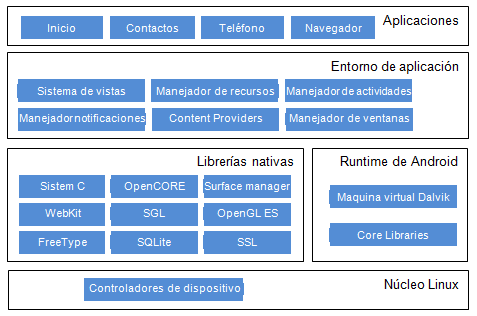
\includegraphics[width=0.58\textwidth]{figuras/docx/arquitectura-android.png}}
    \caption{Arquitectura de Android}
    \label{fig:arquitectura-android}
    \fuente{Gómez (2015).}
\end{figure}

\subsection{Ventajas y limitaciones}

Android destaca por que ofrece ventajas como:

\begin{itemize}
    \item Flexibilidad para funcionar en múltiples tipos de hardware.
    \item Libertad de personalización de interfaz.
    \item Libertad de configuración del sistema.
    \item Compatibilidad amplia con una gran variedad de herramientas y
    servicios de Google.
    \item Alta calidad de gráficos y sonido.
    \item Portabilidad garantizada, ya que sus aplicaciones son desarrolladas en
    Java.
    \item Nivel de seguridad aceptable.
\end{itemize}

Sin embargo, esto también genera limitaciones, como la fragmentación entre
dispositivos y diferentes velocidades en la distribución de actualizaciones del
sistema.

% =====================================================================
\section{Realidad Aumentada}
\label{sec:realidad-aumentada}

La realidad aumentada (RA) es una combinación visual de elementos reales y
virtuales que interaccionan entre ellos (Navarro et~al., 2018),
también es la integración en tiempo real de la información digital en el
entorno de un usuario. La tecnología de RA superpone el contenido al mundo
real, lo que enriquece la percepción de la realidad del usuario en lugar de
reemplazarla (Hayes \& Downie, 2025). A diferencia de la realidad virtual, que
sustituye completamente el entorno físico, la RA superpone información digital
como imágenes, modelos 3D, texto o animaciones sobre la realidad observada
(Azuma, 1997), y hoy se despliega en dispositivos como smartphones, tablets o
lentes inteligentes (Hayes \& Downie, 2025).

\subsection{Componentes de un sistema de Realidad Aumentada}

Un sistema de Realidad Aumentada es una convergencia de hardware y software que
opera un bucle continuo de retroalimentación, en otras palabras, un sistema de
RA debe cumplir con tres características principales, combinar lo real y lo
virtual, operar interactivamente y registrar elementos en 3D (Azuma, 1997).

Un sistema de RA incluye los siguientes componentes esenciales:

\begin{itemize}
    \item \textbf{Dispositivo de visualización:} Permite mostrar la mezcla entre
    la imagen real y los elementos virtuales. Puede ser un teléfono móvil,
    tablet, gafas inteligentes o pantalla montada en la cabeza (Head-Mounted
    Display).
    \item \textbf{Cámara o sensores de captura:} Registra el entorno físico para
    detectar superficies, marcadores o puntos de referencia. Por ejemplo:
    cámaras RGB, sensores de profundidad, giroscopio, acelerómetro.
    \item \textbf{Módulo de seguimiento (tracking):} Se encarga de identificar la
    posición y orientación del usuario o del dispositivo. Esto incluye:
    marker-based, markerless, SLAM, reconocimiento de superficies.
    \item \textbf{Motor de renderizado:} Genera y superpone objetos virtuales en
    el entorno real con coherencia visual y espacial.
    \item \textbf{Interfaz de interacción:} Permite al usuario manipular objetos
    virtuales mediante gestos, toques o movimiento.
\end{itemize}

\subsection{Tecnologías para el desarrollo de Realidad aumentada móvil}

Para el desarrollo móvil, las principales tecnologías de RA son:

\begin{itemize}
    \item \textbf{ARCore:} Es el SDK de realidad aumentada de Google que ofrece
    APIs multiplataforma para crear nuevas experiencias envolventes en Android,
    iOS, Unity y la Web. Transforma la manera en que las personas juegan,
    compran, aprenden, crean y experimentan el mundo juntas mediante la
    comprensión contextual de las personas, los lugares y las cosas
    (Google for Developers, 2025).
    \item \textbf{ARKit:} Es el framework de realidad aumentada de Apple, que
    combina la cámara y los sensores del dispositivo, entre ellos LiDAR en los
    modelos compatibles, para anclar contenido virtual al entorno
    (Apple Inc., 2025). % VERIFICAR contra la página citada (el texto original describía edición de video).
\end{itemize}

Para el desarrollo de este trabajo interesa sobre todo cómo ARCore resuelve el
registro tridimensional. Su seguimiento de movimiento se basa en una técnica de
localización y mapeo simultáneos (SLAM): detecta puntos de interés en la imagen
de la cámara y los combina con los datos inerciales del dispositivo para
estimar su posición y orientación a lo largo del tiempo; además agrupa esos
puntos para reconocer superficies planas, horizontales o verticales (Google for
Developers, s.~f.-e). Sobre ese conocimiento del entorno se pueden crear
\emph{anclas}, es decir, poses fijas respecto del mundo real: a medida que
ARCore refina su estimación del espacio, el ancla se corrige y el contenido
asociado a ella permanece en su lugar en vez de ir a la deriva (Google for
Developers, s.~f.-f). Cuando el dispositivo lo permite, ARCore también estima
la profundidad de la escena comparando imágenes tomadas desde ángulos distintos
mientras la persona mueve el teléfono, con apoyo de aprendizaje automático y,
si existe, de un sensor de tiempo de vuelo; esa información hace que una prueba
de impacto (\emph{hit test}) funcione incluso sobre superficies sin textura
(Google for Developers, s.~f.-b), una técnica que cuenta con descripción en la
literatura científica (Valentin et~al., 2018). Por último, una aplicación puede
declarar ARCore como requerido o como opcional; en el segundo caso sigue
funcionando en teléfonos sin soporte, y las funciones de realidad aumentada
exigen Android 7.0 (API~24) o superior (Google for Developers, s.~f.-c).

\subsection{Alcance de la realidad aumentada en este trabajo}
\label{subsec:ra-alcance}

Un sistema de RA completo exige cumplir las tres características descritas por
Azuma (1997): combinar lo real y lo virtual, ser interactivo en tiempo real y
estar registrado en tres dimensiones. La aplicación las aborda en dos niveles.
En los teléfonos Android compatibles con ARCore, el escáner usa un módulo
nativo propio (\archivo{CoachAR}) que, una vez reconocida la máquina, ancla su
nombre e instrucciones a un punto del entorno real y los mantiene allí mientras
la persona se mueve; esa es la forma de RA con registro tridimensional
(sección~\ref{subsec:it3}). En los demás dispositivos, y cuando el usuario lo
prefiere, el escáner recurre a una cámara convencional con la ficha
superpuesta en pantalla, que satisface la combinación de lo real y lo virtual
y, solo en parte, la interacción en tiempo real.

Conviene tener presentes dos límites. El primero es que el ancla se fija a un
punto de una superficie estimado a partir de la caja delimitadora de la
máquina, no a la geometría de la máquina, y por eso no la sigue si se desplaza.
El segundo es que el reconocimiento ocurre por captura y no de forma continua
sobre el video. En esta memoria el término «realidad aumentada» se usa con
esos matices (sección~\ref{sec:des-alcance}).


% =====================================================================
\section{Inteligencia Artificial}
\label{sec:inteligencia-artificial}

La inteligencia artificial (IA) es una tecnología transformadora que permite a
las máquinas llevar a cabo tareas de resolución de problemas similares a las de
los humanos. Desde el reconocimiento de imágenes y la generación de contenido
creativo hasta la creación de predicciones basadas en datos, la IA permite a
las empresas tomar decisiones más inteligentes a escala (Amazon Web Services, 2025).

La IA consiste en enseñar a las computadoras a hacer las actividades increíbles
que nuestros cerebros pueden hacer, desde comprender el mundo que las rodea
hasta aprender temas nuevos y generar ideas originales (Google Cloud, 2025). En el
contexto de las aplicaciones móviles, la IA permite integrar funciones
avanzadas como la personalización del contenido, la detección automática de
movimiento, el análisis de rendimiento del usuario y la interacción mediante
voz a texto.

\subsection{Aprendizaje automático}

El aprendizaje automático o Machine Learning es una subárea de la inteligencia
artificial dedicado a comprender y construir métodos para imitar la forma en
que aprenden los humanos (Pykes, 2024). El aprendizaje automático, es la
capacidad que tiene un programa para mejorar su desempeño en una tarea a partir
de la experiencia acumulada (Mitchell, 1997).

\subsection{Redes neuronales}

Una red neuronal es un programa o modelo de machine learning que toma
decisiones de forma similar al cerebro humano, al emplear procesos que imitan
la forma en que las neuronas biológicas trabajan juntas para identificar
fenómenos, sopesar opciones y llegar a conclusiones. Se basan en datos de
entrenamiento para aprender y mejorar su precisión con el tiempo (IBM, 2025).

\subsection{Visión por computadora}

La visión artificial es un campo de la inteligencia artificial, que permite a
los ordenadores y sistemas interpretar y analizar datos visuales, así como
también obtener información pertinente a partir de imágenes digitales, videos
y otros datos visuales (Google Cloud, 2025). En el contexto de las aplicaciones
móviles modernas, permite interpretar información visual mediante algoritmos
que detectan objetos, poses, personas entre otras características del entorno.

\subsection{Modelos ligeros para dispositivos móviles}

Los clasificadores de imágenes diseñados para dispositivos móviles equilibran
precisión y consumo de recursos. MobileNetV2 (Sandler et~al., 2018) es una
arquitectura de este tipo, basada en bloques residuales invertidos y cuellos de
botella lineales. Una práctica habitual consiste en reutilizar una red
preentrenada como extractora de características y entrenar solo una capa final
para el problema propio, lo que permite trabajar con pocos datos; los modelos
resultantes pueden ejecutarse en el dispositivo con TensorFlow Lite, sin enviar
imágenes a un servidor.

\subsection{Detección de objetos y la familia YOLO}
\label{subsec:yolo}

Un clasificador responde qué hay en una imagen; un detector de objetos
responde además dónde, pues devuelve para cada objeto una caja delimitadora,
su clase y un grado de confianza. Esa localización es la que permite, en este
proyecto, colocar información junto a la máquina en lugar de limitarse a
nombrarla. YOLO (\emph{You Only Look Once}) planteó la detección como un único
problema de regresión resuelto por una red que mira la imagen completa una sola
vez, lo bastante rápida para el tiempo real (Redmon et~al., 2016). Desde
entonces la familia ha crecido con versiones sucesivas que mejoran la
arquitectura y el entrenamiento (Terven et~al., 2023).

Las versiones recientes se distribuyen mediante la biblioteca Ultralytics, que
reúne en un mismo paquete el entrenamiento, la validación y la exportación a
varios formatos de despliegue (Jocher et~al., 2023). Su código y sus modelos se
publican con licencia AGPL-3.0 o con una licencia empresarial (Ultralytics,
s.~f.-c), condición que debe considerarse si el producto se distribuye fuera
del ámbito académico (sección~\ref{sec:recomendaciones}). YOLO11, la
generación con la que se entrenó una primera versión del detector de este proyecto, incorpora los
bloques C3k2 y un módulo de atención (C2PSA) para extraer mejor las
características, y se ofrece en tamaños desde nano hasta extragrande, de modo
que sirve tanto para dispositivos con pocos recursos como para servidores
(Khanam \& Hussain, 2024). YOLO26, publicada después, elimina la supresión de
no máximos (NMS) durante la inferencia mediante un diseño de doble cabeza,
suprime la pérdida focal de distribución (DFL) para simplificar la cabeza de
detección y la exportación, y se entrena con un optimizador híbrido llamado
MuSGD (Jocher et~al., 2026; Sapkota et~al., 2025). Sus autores reportan una
inferencia en CPU hasta un 43\,\% más rápida que la de YOLO11 en el tamaño
nano (Ultralytics, s.~f.-c). La versión final del detector de este trabajo usa YOLO26 en su tamaño mediano (m). Se trata de preimpresiones y de documentación del
fabricante, aún sin revisión por pares, de modo que esas cifras se toman como
referencia y no como un resultado propio.

Un detector se evalúa con métricas distintas a las de un clasificador. La
intersección sobre la unión (IoU) mide cuánto se solapan la caja predicha y la
real, y una detección se considera correcta si supera un umbral de IoU. La
precisión es la proporción de detecciones correctas entre las emitidas; la
exhaustividad (\emph{recall}), la proporción de objetos reales que se
encontraron; y la precisión promedio (AP) resume el compromiso entre ambas como
el área bajo la curva precisión--exhaustividad. Su promedio entre clases es la
mAP (Padilla et~al., 2021). Es habitual reportar la mAP50 (IoU de al menos 0,5)
y la mAP50--95 (promedio entre umbrales de 0,5 a 0,95), esta última más
exigente con el ajuste de la caja.

Un modelo así puede ejecutarse en el propio teléfono o en un servidor. Ultralytics
Platform permite publicarlo como \emph{endpoint} dedicado: un servicio con
dirección propia, protegido con una clave, que recibe una imagen y devuelve las
detecciones. En su configuración gratuita escala a cero cuando no se usa, por
lo que la primera solicitud tras un período inactivo puede tardar hasta
alrededor de un minuto (Ultralytics, s.~f.-b). Ejecutar el modelo en la nube
permite usar redes más grandes que las que soporta un teléfono, a cambio de
depender de la conexión, aceptar la latencia de red y enviar la imagen a un
servicio externo.

\subsection{Antecedente: visión artificial para la ejecución de ejercicios}

Silva Amado (2024) propone un sistema de visión artificial que estima la pose
con MediaPipe, calcula ángulos articulares y los compara con umbrales para
identificar la ejecución de ejercicios; su evaluación es cualitativa. Este
enfoque verifica \emph{cómo} se ejecuta un movimiento, mientras que el presente
trabajo reconoce \emph{con qué máquina} se entrena y no estima la pose del
usuario (capítulo~\ref{cap:resultados}).

\subsection{Modelos de lenguaje Extenso (LLM)}

Los modelos de lenguaje, son modelos básicos entrenados sobre inmensas
cantidades de datos, lo que los hace capaces de comprender y generar lenguaje
natural y otros tipos de contenido para realizar una amplia variedad de
tareas. Por lo general, los LLM se basan en arquitecturas de aprendizaje
profundo, como Transformer, desarrollado por Google en 2017, y se pueden
entrenar con miles de millones de textos y otros tipos de contenido.

Debido a su escalabilidad, los LLM se pueden entrenar con otros tipos de datos,
como código, imágenes, audio y video, entre otros (Google Cloud, 2025). Su
versatilidad y capacidad de aprendizaje los convierten en herramientas clave en
el desarrollo de aplicaciones modernas, incluyendo sistemas móviles
inteligentes y soluciones que integren realidad aumentada e inteligencia
artificial.

% =====================================================================
\section{Fundamentos del entrenamiento físico}
\label{sec:entrenamiento}

\subsection{Entrenamiento físico}

El entrenamiento es un conjunto de ejercicios y actividades que se realizan
regularmente para mejorar la salud y el estado físico de una persona. Este tipo
de entrenamiento puede incluir variedad de actividades, cada una enfocada en
diferentes aspectos del cuerpo y objetivos personales (Orientanet, s. f.).

Hoy en día, la tecnología como sensores, aplicaciones móviles, realidad
aumentada e inteligencia artificial permiten un monitoreo exhaustivo de la
técnica y el análisis del movimiento, ofreciendo retroalimentación
personalizada en tiempo real. Estas innovaciones pueden optimizar el
rendimiento de los usuarios y ayudar a quienes comienzan en el ejercicio a
realizar las actividades de manera más segura, contribuyendo a reducir el
riesgo de lesiones y a fomentar un estilo de vida saludable.

\subsection{Principios del entrenamiento físico}

El entrenamiento físico está fundamentado en tres principios esenciales, estos
son:

\begin{itemize}
    \item \textbf{Fuerza:} Se centra en incrementar la capacidad del músculo para
    generar tensión, mediante ejercicios con resistencias progresivas. Esto no
    solo mejora el rendimiento deportivo, sino que también contribuye a la salud
    articular y la densidad ósea.
    \item \textbf{Técnica:} Implica la ejecución correcta de cada movimiento para
    maximizar los beneficios y minimizar riesgos. Una técnica adecuada asegura
    que el estímulo recae sobre los músculos deseados y evita compensaciones
    que puedan generar lesiones.
    \item \textbf{Hipertrofia:} Busca aumentar el tamaño del músculo mediante
    cargas, repeticiones y volúmenes adecuados. La hipertrofia requiere un
    equilibrio entre sobrecarga progresiva, nutrición y recuperación para
    generar crecimiento muscular efectivo.
\end{itemize}

\subsection{Biomecánica básica}

La biomecánica estudia el movimiento del cuerpo humano aplicando principios
mecánicos. Comprenderla permite optimizar los ejercicios, analizar palancas,
ángulos de articulaciones y fuerza aplicada, lo que mejora la eficiencia y
reduce el riesgo de lesiones. Los aspectos clave incluyen la alineación
corporal, el centro de gravedad, estabilidad y amplitud de movimiento.

La biomecánica proporciona las bases para corregir patrones de movimiento
disfuncionales, los cuales pueden surgir por hábitos sedentarios,
desequilibrios musculares o mala ejecución repetida de ejercicios. Identificar
estos patrones permite intervenir de manera temprana mediante correcciones
técnicas, fortalecimiento de músculos estabilizadores o ajustes en la postura.

\subsection{Lesiones comunes por mala técnica}

La técnica incorrecta en la ejecución de ejercicios, es una de las principales
causas de las lesiones en entornos de entrenamiento físico, especialmente en
principiantes. La literatura señala que una postura inadecuada, la falta de
control motor y el uso de cargas excesivas incrementan el riesgo de daño
musculoarticular (Kolt \& Snyder-Mackler, 2007).


El desconocimiento de la técnica o la negligencia en la postura pueden provocar
lesiones frecuentes, como:

\begin{itemize}
    \item Dolor lumbar por levantamiento incorrecto de peso.
    \item Tendinitis por movimientos repetitivos sin control.
    \item Esguinces o distensiones musculares por falta de calentamiento o
    postura incorrecta.
    \item Lesiones articulares en hombros, rodillas o muñecas por sobrecarga o
    ángulos inadecuados.
\end{itemize}

Prevenir estas lesiones requiere educación, supervisión y el uso de tecnologías
de monitoreo como sensores de movimiento y análisis de video.

\subsection{Máquinas de gimnasio}

Una máquina de gimnasio es un equipo diseñado para facilitar la realización de
ejercicios físicos de manera controlada, segura y específica. Estas máquinas
están construidas con estructuras metálicas, poleas, cables, placas de peso o
mecanismos electrónicos que permiten guiar el movimiento del usuario. Su diseño
busca aislar determinados grupos musculares, mejorar la estabilidad durante el
ejercicio y proporcionar una carga regulable para adaptarse al nivel de cada
persona.

Las máquinas de gimnasio sirven para entrenar diferentes capacidades físicas
como fuerza, resistencia muscular, estabilidad y acondicionamiento
cardiovascular. Proporcionan un entorno controlado donde el usuario puede
ejecutar movimientos guiados que reducen el riesgo de lesiones, especialmente
en personas principiantes o en rehabilitación. También permiten trabajar grupos
musculares específicos con mayor precisión, mejorar la postura durante el
ejercicio y mantener una progresión segura mediante cargas ajustables. Además,
algunas máquinas monitorean parámetros como ritmo cardíaco, velocidad o
calorías, facilitando el seguimiento del rendimiento.

Las máquinas de gimnasio pueden clasificarse de diversas formas. Según su
función principal, se distinguen las máquinas de fuerza o resistencia, que
utilizan poleas, cables, placas de peso o sistemas hidráulicos para trabajar
grupos musculares específicos (por ejemplo, prensa de piernas, máquina de pecho,
jalón al pecho o curl de bíceps), y las máquinas cardiovasculares, diseñadas
para mejorar la resistencia cardiorrespiratoria y quemar calorías (caminadoras,
bicicletas estáticas, elípticas y remadoras). Según el tipo de movimiento,
pueden ser de movimiento guiado, en las que la máquina controla la trayectoria
y que son ideales para principiantes, o de movimiento libre asistido, que
permiten mayor libertad pero brindan estabilidad adicional. Según el mecanismo
de resistencia, pueden funcionar con placas de peso (weight stack), peso libre
integrado, sistemas hidráulicos o resistencia electromagnética, esta última
común en las máquinas cardiovasculares modernas. Finalmente, según el área del
cuerpo que trabajan, se agrupan en máquinas para tren superior (pecho, espalda,
hombros y brazos), tren inferior (piernas y glúteos) y core (abdominales y zona
lumbar).

\subsection{Prescripción del entrenamiento de fuerza}
\label{subsec:prescripcion}

La prescripción del entrenamiento de fuerza se define mediante variables como la
selección de ejercicios, la intensidad, el volumen, la frecuencia semanal y los
descansos, y requiere una progresión gradual de la carga (Kraemer \&
Ratamess, 2004). Estas pautas, consolidadas en la literatura, son la base de
conocimiento del generador de rutinas del sistema
(sección~\ref{sec:des-alcance}).

\subsection{Indicadores nutricionales y metabólicos}
\label{subsec:nutricion}

El índice de masa corporal (IMC) relaciona el peso con la estatura y se clasifica
con los puntos de corte de la Organización Mundial de la Salud (2000). Para
estimar el gasto energético en reposo, y con él las metas calóricas diarias, se
utiliza la ecuación predictiva de Mifflin et~al. (1990), desarrollada en
personas sanas. Ambos indicadores son orientativos y no reemplazan la
valoración de un profesional de la nutrición.

% =====================================================================
\section{Plataforma de desarrollo}
\label{sec:plataforma}

\subsection{Visual Studio Code}

Visual Studio Code es un editor de código fuente creado por Microsoft,
diseñado para ser ligero, rápido y altamente personalizable (Cuadrado, 2022).
Sirve para escribir, corregir y organizar programas en muchos lenguajes como
Java, Python, C++, entre otros. Este funciona en Windows, Mac y Linux.

A diferencia de un IDE tradicional que viene completo desde la instalación, VS
Code parte de un núcleo ligero y va incorporando funcionalidad mediante
extensiones, lo que permite adaptarlo a prácticamente cualquier lenguaje o
framework sin cargar con herramientas que el proyecto no necesita.

% =====================================================================
\section{Frameworks para desarrollo Mobile}
\label{sec:frameworks}

El desarrollo de aplicaciones móviles ha evolucionado en gran manera gracias a
la aparición de frameworks que permiten crear interfaces eficientes,
multiplataforma y optimizadas para dispositivos con recursos limitados. Estos
frameworks ofrecen herramientas, bibliotecas y entornos de trabajo que
simplifican el proceso de creación de aplicaciones al abstraer componentes
nativos y proporcionar estructuras reutilizables.

Entre los frameworks más utilizados se encuentran React Native, Flutter, Ionic,
Xamarin y Jetpack Compose.

La descripción, características y ventajas de cada uno de estos frameworks se comparan en la Tabla~\ref{tab:frameworks} del Anexo~\ref{anx:comparativas}.

\subsection{React Native}

React Native es un framework para la creación de aplicaciones nativas para iOS
y Android, creado por Meta (Facebook). Permite construir aplicaciones
multiplataforma utilizando JavaScript y React. A diferencia de las soluciones
híbridas tradicionales, React Native genera interfaces nativas, lo que permite
lograr un rendimiento cercano al desarrollo completamente nativo (React Native,
2025).

React Native se caracteriza por (Viera, s. f.):

\begin{itemize}
    \item \textbf{Componentes nativos:} Usa componentes de interfaz de usuario
    nativo en lugar de componentes web.
    \item \textbf{Hot reloading:} Permite ver cambios en tiempo real sin
    recompilar toda la app, acelerando el desarrollo.
    \item \textbf{Acceso a APIs nativas:} Permite integrar funcionalidades como
    cámara, GPS y notificaciones directamente del dispositivo.
    \item \textbf{Desarrollo Multiplataforma:} Escribe una sola vez y ejecuta en
    ambas plataformas (iOS y Android).
    \item \textbf{Gran Comunidad:} Amplia comunidad de desarrolladores y recursos
    disponibles.
    \item \textbf{Rendimiento:} Ofrece un rendimiento cercano al nativo gracias a
    su arquitectura.
    \item \textbf{Interfaz de Usuario:} Permite crear interfaces de usuario ricas
    y fluidas.
    \item \textbf{Integración con Librerías:} Compatible con librerías de
    terceros y APIs nativas.
    \item \textbf{Soporte para TypeScript:} Permite usar TypeScript para un
    desarrollo más robusto y seguro.
\end{itemize}

% =====================================================================
\section{Bases de datos de aplicaciones Móviles}
\label{sec:bases-datos}

Las bases de datos desempeñan un papel fundamental en el desarrollo de
aplicaciones móviles, ya que permiten almacenar, administrar y sincronizar la
información que utiliza el sistema durante su funcionamiento.

En el entorno móvil actual existen múltiples opciones tecnológicas, entre las
cuales destacan Firebase Firestore, SQLite, MongoDB Atlas, MySQL y PostgreSQL.

La descripción, características y ventajas de cada una de estas bases de datos se comparan en la Tabla~\ref{tab:bases-datos} del Anexo~\ref{anx:comparativas}.

\subsection{Firebase}

Firebase es una plataforma en la nube desarrollada por Google, facilita el
desarrollo de aplicaciones, bases de datos en tiempo real, autenticación y
hosting. Esta herramienta permite enviar notificaciones push y analizar el
rendimiento de las apps (Isaac, 2025).

En la actualidad, Firebase integra servicios modernos como Cloud Firestore,
Google Analytics 4, App Check, Data Connect y Firebase Studio, lo que la
convierte en una solución completa para proyectos actuales que buscan
escalabilidad, seguridad y analítica avanzada (López Mora, 2025).

% =====================================================================
\section{Herramientas}
\label{sec:herramientas}

\subsection{Control de versiones}

El control de versiones es un sistema que ayuda a rastrear y gestionar los
cambios realizados en un archivo o conjunto de archivos, principalmente
utilizado por ingenieros de software para hacer seguimiento a las
modificaciones realizadas en el código fuente (B, 2025).

En este proyecto se utilizaron:

\begin{enumerate}
    \item \textbf{Git:} Es un sistema de control de versiones distribuido,
    gratuito y de código abierto diseñado para manejar proyectos pequeños, como
    también proyectos muy grandes de forma rápida y eficiente (Git, s. f.).
    \item \textbf{GitHub:} Es un servicio basado en la nube que aloja un sistema
    de control de versiones (VCS) llamado Git. Éste permite a los
    desarrolladores colaborar y realizar cambios en proyectos compartidos, a la
    vez que mantienen un seguimiento detallado de su progreso (B, 2025).
\end{enumerate}

\subsection{Herramientas de Gestión}

Las herramientas de gestión de proyectos están especialmente diseñadas para
asistir a un empleado o equipo en la gestión eficaz de sus proyectos y tareas
(Gurnov \& Wrike, 2025). Estas herramientas son utilizadas para la
organización, planificación, seguimiento y aseguramiento de calidad del
proyecto.

\begin{itemize}
    \item \textbf{Trello:} Es una herramienta flexible para la gestión del
    trabajo, basado en tableros Kanban que facilita la organización visual de
    tareas mediante listas y tarjetas (Atlassian, 2023). Su enfoque intuitivo
    permite coordinar actividades, asignar responsabilidades y monitorear el
    avance de cada fase del proyecto.
\end{itemize}

\chapter{ÁREA DE APLICACIÓN}
\label{cap:area-aplicacion}

El presente capítulo describe el enfoque metodológico adoptado para el
desarrollo del sistema inteligente de entrenamiento en gimnasios con realidad
aumentada e inteligencia artificial. El propósito es garantizar un proceso de
construcción ordenado, iterativo y orientado a la calidad, acorde a las
necesidades específicas del desarrollo móvil. Para ello, se selecciona la
metodología ágil Mobile-D, diseñada especialmente para proyectos móviles con
ciclos de producción rápidos, entregas frecuentes y constante
retroalimentación.

% =====================================================================
\section{Antecedentes}
\label{sec:aa-antecedentes}

\subsection{Enfoque metodológico}

La metodología es el conjunto de procedimientos, técnicas y estrategias que
orienta la ejecución de un proyecto de investigación o desarrollo tecnológico.
En el presente trabajo, el enfoque metodológico define la manera en que se
estructura el proceso de diseñar, desarrollar y evaluar el sistema. El proyecto
adopta un enfoque cuantitativo-aplicado porque se medirá métricas objetivas del
sistema inteligente, como también se realizará la creación de una solución
tecnológica concreta mediante el uso de técnicas de ingeniería de software,
inteligencia artificial y realidad aumentada. En este caso, se emplean
fundamentos de biomecánica, visión por computadora, aprendizaje automático y
diseño de software para desarrollar una herramienta que facilite el uso
correcto de máquinas, la corrección técnica de ejercicios y la personalización
del entrenamiento.

% =====================================================================
\section{Metodología de desarrollo}
\label{sec:aa-metodologia}

La metodología Mobile-D fue seleccionada para guiar el proceso de desarrollo
del sistema debido a que está específicamente diseñada para proyectos de
software orientados a dispositivos móviles, caracterizados por ciclos de
producción rápidos, restricciones de hardware y cambios frecuentes en los
requerimientos.

Mobile-D es una metodología ágil diseñada para el desarrollo de aplicaciones
móviles, que requiere ciclos de entrega cortos, validación continua, pruebas en
dispositivos reales y flexibilidad ante cambios de interfaz o funcionalidad. El
presente proyecto integra módulos de guía interactiva mediante imágenes,
animaciones o realidad aumentada, generación de rutinas personalizadas mediante
inteligencia artificial, herramientas de seguimiento físico y una interfaz
altamente intuitiva.

Mobile-D permite abordar de forma progresiva y controlada, los elementos
principales del proyecto:

\begin{itemize}
    \item La guía visual sobre el uso correcto de máquinas y la ejecución de
    ejercicios, que exige pruebas de usabilidad desde las primeras etapas.
    \item La generación de rutinas personalizadas mediante algoritmos de IA,
    cuya precisión y utilidad deben ajustarse iterativamente.
    \item Los módulos de planificación y seguimiento, que requieren
    refinamientos sucesivos para asegurar claridad, funcionalidad y coherencia
    en la experiencia del usuario.
    \item La interfaz móvil, que debe ser evaluada continuamente para
    garantizar facilidad de uso, accesibilidad y entendimiento para usuarios
    principiantes.
\end{itemize}

% =====================================================================
\section{Aplicación de la Metodología Mobile-D}
\label{sec:aa-aplicacion-mobiled}

La metodología Mobile-D se implementa en el presente proyecto mediante cinco
fases que permiten estructurar el desarrollo de la aplicación de manera
incremental, verificable y orientada a la calidad. A continuación, se detalla
la aplicación específica de cada fase al sistema inteligente de entrenamiento.

% ---------------------------------------------------------------------
\subsection{Fase de Exploración}

En esta etapa se definen las bases conceptuales, técnicas y organizativas del
presente proyecto.

\titulillo{Módulos principales del sistema}

El sistema propuesto está compuesto por los siguientes módulos esenciales:

\begin{itemize}
    \item Registro y autenticación de usuarios.
    \item Guía detallada del uso correcto de máquinas de gimnasio.
    \item Ejecución técnica correcta de ejercicios específicos.
    \item Rutinas personalizadas mediante inteligencia artificial.
    \item Registro nutricional básico (calorías diarias).
    \item Seguimiento del progreso físico (peso, IMC, medidas).
    \item Reportes estadísticos y visualización del avance.
\end{itemize}

\titulillo{Requerimientos de sistema}

\textit{Requerimientos Funcionales}

\begin{itemize}
    \item RF1: Registrar y autenticar usuarios mediante correo y contraseña.
    \item RF2: Mostrar información técnica y visual de cada máquina de gimnasio.
    \item RF3: Generar rutinas personalizadas mediante IA según edad, peso, nivel
    y objetivo.
    \item RF4: Registrar peso, estatura, IMC y progreso físico.
    \item RF5: Registrar ingesta calórica diaria del usuario.
    \item RF6: Visualizar reportes y estadísticas del progreso físico.
\end{itemize}

\textit{Requerimientos No Funcionales}

\begin{itemize}
    \item RNF1: La aplicación debe ejecutarse en Android versión 8.0 o superior.
    \item RNF2: La interfaz debe ser intuitiva, rápida y adaptable a diferentes
    pantallas.
    \item RNF3: La sincronización de datos debe realizarse en tiempo real
    mediante Firebase.
\end{itemize}

\titulillo{Selección de Tecnologías}

\textit{Frontend}

\begin{itemize}
    \item \textbf{React Native:} Es un framework multiplataforma, que permite
    desarrollar aplicaciones móviles para dispositivos Android.
    \item \textbf{TypeScript:} Lenguaje de programación principal para el
    desarrollo de las interfaces y la lógica del lado del cliente.
    \item \textbf{Figma:} Herramienta de diseño utilizada para crear prototipos
    interactivos, pantallas iniciales, facilitando la validación visual del
    producto.
\end{itemize}

\textit{Backend}

\begin{itemize}
    \item \textbf{Firebase Authentication:} Servicio que permite gestionar el
    registro, inicio de sesión y recuperación de credenciales de forma segura.
    \item \textbf{Firebase Firestore:} Base de datos NoSQL en la nube que
    proporciona sincronización en tiempo real y escalabilidad para manejar
    información de usuarios, ejercicios, rutinas y progreso.
    \item \textbf{Firebase Storage:} Servicio destinado al almacenamiento de
    imágenes, animaciones y videos que acompañan la guía técnica del sistema.
    \item \textbf{TensorFlow Lite:} Biblioteca optimizada para ejecutar modelos
    de inteligencia artificial directamente en el dispositivo móvil, utilizada
    para recomendar la estructura de las rutinas a partir de los parámetros del
    usuario y para reconocer la máquina a partir de una fotografía.
\end{itemize}

% ---------------------------------------------------------------------
\subsection{Fase de Inicialización}

En esta fase se prepara el entorno de desarrollo, la planificación inicial y la
definición de la arquitectura del sistema. También se establecen los
lineamientos de codificación y los mecanismos de control de versiones (Git).

\titulillo{Configuración del entorno}

Las principales actividades a realizar para la preparación del ambiente, son:

\begin{itemize}
    \item Instalación de Node.js.
    \item Instalación de Expo CLI.
    \item Creación de proyecto en Firebase y configuración de los servicios de
    autenticación, Firestore y Storage.
    \item Integración de la librería de TensorFlow Lite.
    \item Creación del repositorio en GitHub y definición de las ramas
    principales.
\end{itemize}

\titulillo{Arquitectura del sistema}

La arquitectura definida para el desarrollo de la aplicación es el de
cliente-servidor, donde la aplicación móvil actúa como cliente y los servicios
en la nube proporcionan autenticación, almacenamiento de datos, persistencia
multimedia, mientras que los modelos de IA se ejecutan en el propio dispositivo.

La arquitectura cliente servidor permite garantizar escalabilidad,
sincronización en tiempo real y disponibilidad permanente del servicio.

La estructura detallada de esta arquitectura, organizada en capas de
presentación, lógica de negocio, servicios e inteligencia artificial, se
describe en la sección~\ref{sec:des-arquitectura} del
Capítulo~\ref{cap:desarrollo}, como parte de la fase de inicialización.

% ---------------------------------------------------------------------
\subsection{Fase de Producción}

Esta es la etapa central del desarrollo. Dentro de esta etapa se implementan
los módulos de IA, seguimiento físico y rutinas personalizadas. Esta fase de
producción se organiza en iteraciones cortas, cada una de las cuales agrega un
conjunto de funcionalidades al sistema.

\titulillo{\textit{Día de prueba}}

En este día se verifica que toda la plataforma técnica funcione correctamente
antes de empezar a desarrollar funcionalidades reales.

Se debe realizar las siguientes acciones:

\begin{itemize}
    \item \textbf{Verificación de la integración con Firebase}

    Se realizarán pruebas básicas con los servicios principales de Firebase
    para garantizar su correcto funcionamiento:
    \begin{itemize}
        \item \textbf{Authentication:} creación de usuarios de prueba,
        validación de inicio de sesión y manejo de errores.
        \item \textbf{Firestore:} creación de colecciones temporales, escritura
        y lectura de documentos, y verificación de permisos básicos.
        \item \textbf{Storage:} carga y visualización de archivos multimedia
        para garantizar el acceso correcto al módulo de almacenamiento.
    \end{itemize}
    Estas pruebas aseguran que la aplicación pueda gestionar información real
    durante la fase de producción.
\end{itemize}

\textbf{Validación del entorno móvil}

Se verifica la correcta compilación del proyecto tanto en un dispositivo físico
como en un emulador. Además, se comprueba la navegación entre pantallas
iniciales y la ejecución estable del entorno Expo.

\textbf{Prueba preliminar del modelo TensorFlow Lite}

Se verifica la carga del modelo de inteligencia artificial y su ejecución
básica en el dispositivo, con el fin de confirmar la compatibilidad entre
TensorFlow Lite y la plataforma móvil utilizada.

\textbf{Validación del control de versiones}

Se realiza una prueba de uso del repositorio GitHub, asegurando que se pueden
subir y descargar cambios correctamente, lo cual es indispensable para mantener
un desarrollo organizado.

\titulillo{\textit{Día de salida}}

En este día se cierra la fase de inicialización, aquí no se realizan pruebas
sino ajustes finales y organización para dejar el proyecto listo para comenzar
la fase de producción.

Para esto, se debe realizar:

\textbf{Organización y limpieza del proyecto}

Se reorganiza la estructura interna del proyecto siguiendo la arquitectura
definida, agrupando componentes, servicios, pantallas y modelos de datos en
carpetas específicas. Asimismo, se eliminaron archivos temporales o de prueba
utilizados en fases previas.

\textbf{Configuración de variables y llaves de entorno}

Se definieron archivos seguros para almacenar las credenciales de Firebase y
otras configuraciones sensibles, evitando que estas sean expuestas en el
repositorio de código.

\textbf{Creación de ramas base de desarrollo en GitHub}

Se estableció una estructura de ramas para gestionar el desarrollo:

\begin{itemize}
    \item \texttt{main}: versión estable.
    \item \texttt{develop}: versión en progreso.
    \item \texttt{feature/nombre-del-módulo}: para cada nueva funcionalidad.
\end{itemize}

Esta estructura permite un control ordenado de versiones.

% ---------------------------------------------------------------------
\subsection{Fase de Estabilización}

Dentro de esta fase se integran y verifican los componentes desarrollados,
asegurando consistencia, rendimiento y compatibilidad entre módulos. Las
pruebas de usabilidad y validación funcional se intensifican.

Las actividades a realizarse en esta fase son:

\begin{itemize}
    \item Refactorizar código para mejorar legibilidad.
    \item Optimizar carga de imágenes y videos.
    \item Ajustar tiempos de respuesta del sistema.
    \item Revisar el diseño visual para mejorar usabilidad.
    \item Corregir detalles detectados durante las pruebas en dispositivos
    reales.
\end{itemize}

% ---------------------------------------------------------------------
\subsection{Fase de Pruebas del sistema}

Se ejecutan pruebas de aceptación, evaluación del modelo de IA, pruebas en
dispositivos reales y corrección final de errores. El objetivo es garantizar
que el sistema sea estable y esté listo para su uso práctico.

Esto mediante las siguientes pruebas:

\begin{itemize}
    \item \textbf{Pruebas Funcionales:} Las pruebas funcionales son un tipo de
    verificación que evalúa si el sistema cumple correctamente con los
    requerimientos establecidos, las pruebas funcionales se basan en técnicas
    de caja negra, donde el evaluador verifica funciones, escenarios y
    respuestas del sistema desde la perspectiva del usuario final (IEEE, 1990).
    \item \textbf{Pruebas de Usabilidad:} Las pruebas de usabilidad se enfocan
    en analizar qué tan fácil, eficiente y satisfactoria es la interacción de un
    usuario con la interfaz del sistema. Se fundamenta en principios como
    facilidad de aprendizaje, eficiencia, reducción de errores y satisfacción
    del usuario (Nielsen, 1993).
    \item \textbf{Pruebas de Aceptación:} Las pruebas de aceptación validan que
    el sistema completo cumpla con los requerimientos acordados, estas pruebas
    representan la etapa final de validación del producto e incluyen la
    ejecución de escenarios reales que reflejan el uso cotidiano de la
    aplicación (Pressman, 2010).
\end{itemize}

% =====================================================================
\section{Roles}
\label{sec:aa-roles}

Dentro de la metodología Mobile-D, los roles cumplen la función de organizar
las responsabilidades durante el desarrollo del proyecto, aun cuando éste sea
desarrollado por una sola persona.

A continuación, se describen los roles adoptados en el proyecto:

\begin{table}[H]
\centering
\begin{tabularx}{\textwidth}{|L{3.6cm}|Y|L{3cm}|}
\hline
\rowcolor{encabezado} \textbf{Rol} & \textbf{Responsabilidades} & \textbf{Responsable} \\
\hline
Product Owner & Define alcance, objetivos y prioridades del sistema & Erika
Chino \\ \hline
Arquitecto Mobile & Diseña la arquitectura y selecciona las tecnologías & Erika
Chino \\ \hline
Desarrollador móvil & Implementa módulos, interfaces y lógica de negocio &
Erika Chino \\ \hline
Diseñador UI/UX & Diseña prototipos, navegación y experiencia de usuario &
Erika Chino \\ \hline
QA Tester & Realiza pruebas funcionales, de usabilidad y rendimiento & Erika
Chino \\
\hline
\end{tabularx}
\caption[Roles establecidos por Mobile-D]{Roles establecidos por Mobile-D. \textit{Fuente:} Elaboración propia.}
\label{tab:roles}
\end{table}

% =====================================================================
\section{Técnicas e instrumentos de recolección de información}
\label{sec:aa-tecnicas}

Para fundamentar el diseño y funcionamiento del sistema se utilizarán las
siguientes técnicas:

\begin{itemize}
    \item \textbf{Revisión documental:} Investigación de aplicaciones similares,
    biomecánica, técnica correcta de ejercicios y libros especializados.
    \item \textbf{Observación directa:} Registro del uso real de máquinas en
    gimnasios locales.
    \item \textbf{Entrevistas informales:} Conversaciones con usuarios
    principiantes para conocer sus dificultades reales en el gimnasio.
    \item \textbf{Prototipado:} Elaboración de pantallas en Figma para validar
    la experiencia de usuario antes del desarrollo.
\end{itemize}

\chapter{DESARROLLO DEL PROYECTO}
\label{cap:desarrollo}

% Los archivos del capítulo se encuentran en capitulos/cap4/.
% Las marcas \pendiente{...} en rojo indican datos que solo
% la autora puede completar (capturas de pantalla, resultados en dispositivos
% reales, pruebas con usuarios). Para ocultarlas todas antes de la entrega:
% \renewcommand{\pendiente}[1]{} en config/comandos.tex.

En este capítulo se describe el desarrollo del sistema según las fases de
la metodología Mobile-D. Se detallan las actividades de cada fase, los
artefactos obtenidos y la aplicación de los fundamentos del marco referencial.
El desarrollo del sistema busca cumplir los objetivos del proyecto y dar
respuesta a la problemática planteada.

% =====================================================================
%  FASE DE EXPLORACIÓN (versión actualizada). Cambios respecto al original:
%   - Realidad aumentada: se corrige «el usuario siempre confirma la máquina»
%     (con confianza >= 0,8 la app acepta la sugerencia) y se acota el término
%     según Azuma (1997).
%   - Actores y tecnologías: Cloud Functions y App Check; USDA vía función.
%   - Fuentes de datos: se añaden ExerciseDB y Gym Visual; «s.f.» -> «s. f.».
%   - RNF1: mínimo de Android = 7.0 (API 24), valor por defecto de React Native.
%   - Persistencia sin conexión: capacidad del SDK, no activada en la app.
%   - Cronograma: solicitudes de integración #5, #6 y #7.
% =====================================================================
% =====================================================================
\section{Fase de Exploración}
\label{sec:des-exploracion}

En esta fase se definen los requerimientos, el alcance y las tecnologías para el desarrollo
del producto.

\subsection{Establecimiento de los interesados}

Tutor del proyecto(Cliente): Ing. Jimmy Villarroel Novillo.

\subsection{Actores del sistema}

El actor principal del sistema es el usuario, quien completa su perfil,
consulta las instrucciones para el uso correcto de las máquinas del gimnasio y genera 
rutinas de entrenamiento personalizadas. Además, puede registrar su consumo
calórico, consultar su índice de masa corporal (IMC) y hacer un seguimiento
de su progreso físico.

\subsection{Roles y Tareas}

Para el desarrollo del sistema se han identificado los siguientes usuarios:

\begin{table}[htbp]
\centering
\begin{tabular}{|p{0.18\linewidth}|p{0.49\linewidth}|p{0.21\linewidth}|}
  \hline
  \textbf{Nombre} & \textbf{Descripción} & \textbf{Stakeholder} \\
  \hline
  Usuario Final & 
  Completa su perfil físico, consulta las instrucciones para el uso correcto
  máquinas del gimnasio, escanea máquinas, obtiene y planifica sus rutina, registra 
  su consumo calórico, consulta su índice de masa corporal IMC y revisa su progreso físico. & 
  Persona que entrena en el gimnasio\\
  \hline
  \end{tabular}
  \caption{Roles y tareas de Coach App (Elaboración propia)}
  \label{tab:roles-tareas}
\end{table}


\subsection{Requerimientos iniciales} 

En esta etapa se elabora la primera definición de los requerimientos. Los requerimientos 
funcionales describen las acciones que la aplicación debe permitir al usuario, mientras que
los no funcionales establecen las condiciones de calidad que debe cumplir.
Esta definición inicial delimita el alcance del sistema y sirve de base para su diseño y desarrollo.

\subsubsection{Requerimientos funcionales}

Los requerimientos funcionales describen las funciones que la aplicación debe ofrecer al usuario. 
La siguiente tabla presenta los requerimientos generales y sus respectivos subrequerimientos.

\begin{longtable}{|L{2.2cm}|L{10.8cm}|}
\hline
\rowcolor{encabezado}
\textbf{\textcolor{black}{CÓDIGO}} &
\textbf{\textcolor{black}{DESCRIPCIÓN}} \\
\hline
\endfirsthead

\hline
\rowcolor{encabezado}
\textbf{\textcolor{black}{CÓDIGO}} &
\textbf{\textcolor{black}{DESCRIPCIÓN}} \\
\hline
\endhead

\endfoot

\caption{Requerimientos funcionales del sistema (elaboración propia)}
\label{tab:rf}\\
\endlastfoot

RF1.1 & Permitir el registro de un usuario con nombre, apellido,
correo electrónico y contraseña. \\
\hline
RF1.2 & Permitir el inicio de sesión mediante correo electrónico y
contraseña o mediante una cuenta de Google. \\
\hline
RF1.3 & Permitir la recuperación de la contraseña por correo
electrónico y el cierre de sesión. \\
\hline
RF1.4 & Permitir que el usuario registre, en su primer ingreso, su
objetivo de entrenamiento, nivel de experiencia, edad, estatura, peso
y días disponibles para entrenar. \\
\hline
RF1.5 & Permitir la consulta y edición de los datos del perfil. \\
\hline

RF2.1 & Permitir la búsqueda de máquinas por texto, con o sin tildes,
y el filtrado del catálogo por grupo muscular y tipo de equipo. \\
\hline
RF2.2 & Mostrar la ficha de cada máquina con su descripción, los
músculos trabajados, las instrucciones de uso, los errores comunes,
las recomendaciones para prevenir lesiones y las variantes comerciales. \\
\hline
RF2.3 & Mostrar los ejercicios asociados a cada máquina con su
animación, músculo objetivo y nivel de dificultad. \\
\hline
RF2.4 & Permitir el escaneo de una máquina con la cámara y mostrar
su ficha sobre la imagen en vivo. Si el sistema no logra identificarla
automáticamente, permitir que el usuario la seleccione de una lista. \\
\hline

RF3.1 & Generar una rutina semanal según el objetivo de entrenamiento
y el nivel de experiencia del usuario. \\
\hline
RF3.2 & Permitir la creación y eliminación de rutinas personalizadas
organizadas por días, con series, repeticiones y tiempos de descanso
para cada ejercicio. \\
\hline
RF3.3 & Permitir que el usuario agregue ejercicios a su rutina desde
la ficha de una máquina y marque una rutina como activa. \\
\hline

RF4.1 & Calcular el índice de masa corporal (IMC), clasificar el
resultado según los criterios de la OMS y guardar el historial de
cálculos. \\
\hline
RF4.2 & Permitir el registro del peso, la estatura y las notas de
progreso físico, con cálculo automático del IMC. \\
\hline

RF5.1 & Permitir la búsqueda de alimentos en español y el registro
de la cantidad consumida en gramos. Calcular las calorías y los
macronutrientes de la porción registrada. \\
\hline
RF5.2 & Permitir que el usuario agregue alimentos de consumo frecuente
con un toque o registre un alimento manualmente. \\
\hline
RF5.3 & Mostrar el consumo diario de calorías y macronutrientes en
relación con las metas del usuario y permitir la eliminación de
registros. \\
\hline

RF6.1 & Mostrar en un gráfico la evolución del peso y del IMC, e
indicar la variación acumulada y la categoría actual del IMC. \\
\hline
RF6.2 & Permitir que el usuario marque como completado el entrenamiento
del día y consulte su racha, los días entrenados durante la semana y
el total de entrenamientos completados. \\
\hline
\end{longtable}

\subsubsection{Requerimientos no funcionales}

Los requerimientos no funcionales establecen las condiciones de calidad
que debe cumplir la aplicación. La tabla siguiente describe cada requerimiento.

\begin{longtable}{|L{2.2cm}|L{10.8cm}|}
\hline
\rowcolor{encabezado}
\textbf{\textcolor{black}{CÓDIGO}} &
\textbf{\textcolor{black}{DESCRIPCIÓN}} \\
\hline
\endfirsthead

\hline
\rowcolor{encabezado}
\textbf{\textcolor{black}{CÓDIGO}} &
\textbf{\textcolor{black}{DESCRIPCIÓN}} \\
\hline
\endhead

\endfoot

\caption{Requerimientos no funcionales del sistema (elaboración propia)}
\label{tab:rnf}\\
\endlastfoot

RNF1 & \textbf{Portabilidad.} La aplicación debe poder instalarse y
ejecutarse en dispositivos con Android 7.0 (API 24) o superior. \\
\hline

RNF2 & \textbf{Usabilidad.} La interfaz debe presentarse en español,
adaptarse a distintos tamaños de pantalla y permitir el acceso a los
módulos principales mediante pestañas de navegación. \\
\hline

RNF3 & \textbf{Fiabilidad.} Los cambios guardados en las rutinas, los
registros y los entrenamientos deben sincronizarse mediante Firebase
y reflejarse en pantalla sin que el usuario tenga que recargarla
manualmente. \\
\hline

RNF4 & \textbf{Seguridad.} Cada usuario debe poder consultar y modificar
únicamente sus propios datos. El catálogo debe ser de solo lectura
para los usuarios de la aplicación. Las reglas de Firestore deben
validar los tipos y rangos de los datos al guardar los cambios. \\
\hline

RNF5 & \textbf{Eficiencia.} El catálogo de máquinas debe descargarse
una sola vez por sesión y reutilizarse al volver a consultarlo.
Las URL de las imágenes deben conservarse en caché para reducir
las solicitudes repetidas. \\
\hline

RNF6 & \textbf{Mantenibilidad.} El código debe escribirse en TypeScript
con el modo estricto habilitado y organizarse según las capas del
patrón MVC. La comprobación de tipos y el análisis estático deben
completarse sin errores. \\
\hline
\end{longtable}

\subsubsection{Análisis de los requerimientos mediante casos de uso}

La Figura~\ref{fig:casos-uso} presenta el diagrama de casos de uso del
sistema. El actor principal es el usuario; Firebase y las APIs externas
participan como actores secundarios.

\begin{figure}[!t]
\centering
\begin{tikzpicture}[font=\footnotesize, lbl/.style={font=\scriptsize, fill=white, inner sep=1pt}]
  \actor{usr}{(0,-0.4)}{Usuario}
  \actor{fb}{(13.8,2.2)}{Firebase}
  \actor{api}{(13.8,-3.0)}{APIs externas}
  \node[draw, rounded corners, minimum width=9.8cm, minimum height=13.6cm,
        label={[font=\small\bfseries]above:Sistema \nombreApp}] (sis) at (6.75,-0.4) {};
  \node[casouso] (u1)  at (4.2, 5.6) {Registrarse / iniciar sesión};
  \node[casouso] (u2)  at (4.2, 4.4) {Completar \emph{onboarding}};
  \node[casouso] (u3)  at (4.2, 3.2) {Consultar guía de máquinas};
  \node[casouso] (u4)  at (4.2, 2.0) {Escanear máquina (RA)};
  \node[casouso] (u5)  at (4.2, 0.8) {Generar rutina automática};
  \node[casouso] (u6)  at (4.2,-0.4) {Crear rutina personalizada};
  \node[casouso] (u7)  at (4.2,-1.6) {Calcular IMC};
  \node[casouso] (u8)  at (4.2,-2.8) {Registrar progreso físico};
  \node[casouso] (u9)  at (4.2,-4.0) {Registrar alimentos};
  \node[casouso] (u10) at (4.2,-5.2) {Marcar entrenamiento};
  \node[casouso] (u11) at (4.2,-6.4) {Gestionar perfil};
  \node[casouso] (v1) at (9.3, 3.2) {Ver ficha y ejercicios};
  \node[casouso] (v2) at (9.3, 2.0) {Agregar ejercicio a rutina};
  \node[casouso] (v7) at (9.3, 0.8) {Obtener ejercicios (wger)};
  \node[casouso] (v3) at (9.3,-0.4) {Activar rutina};
  \node[casouso] (v5) at (9.3,-2.8) {Ver reporte de progreso};
  \node[casouso] (v4) at (9.3,-4.0) {Buscar alimento (USDA)};
  \node[casouso] (v6) at (9.3,-5.2) {Ver racha semanal};
  \foreach \u in {u1,u2,u3,u4,u5,u6,u7,u8,u9,u10,u11} \draw (usr) -- (\u.west);
  \draw[flechad] (u3) -- node[lbl, above=1pt]{«include»} (v1);
  \draw[flechad] (v2) -- node[lbl, right=1pt]{«extend»} (v1);
  \draw[flechad] (u5) -- node[lbl, above=1pt]{«include»} (v7);
  \draw[flechad] (v3) -- node[lbl, above=1pt]{«extend»} (u6);
  \draw[flechad] (v5) -- node[lbl, above=1pt]{«extend»} (u8);
  \draw[flechad] (u9) -- node[lbl, above=1pt]{«include»} (v4);
  \draw[flechad] (v6) -- node[lbl, above=1pt]{«extend»} (u10);
  \draw (v1.east) -- (fb);
  \draw (v5.east) -- (fb);
  \draw (v7.east) -- (api);
  \draw (v4.east) -- (api);
\end{tikzpicture}
\caption{Diagrama de casos de uso del sistema}
\label{fig:casos-uso}
\fuente{Elaboración propia.}
\end{figure}

\clearpage
\subsection{Definición del alcance}
\label{sec:des-alcance}

El alcance del proyecto se determina a través de sus limitaciones:

\subsubsection{Limitaciones}

Las limitaciones de la aplicación desarrollada son:

\begin{itemize}
    \item La aplicación solo puede ser ejecutada en dispositivos con el sistema operativo Android.

    \item El reconocimiento de máquinas en la nube y la búsqueda de
    alimentos requieren conexión a internet.

    \item El escaneo de máquinas requiere acceso a la cámara. El anclaje
    de la ficha al entorno solo está disponible en dispositivos
    compatibles con ARCore.

    \item El reconocimiento automático se limita a los tipos de máquinas
    incluidos en el entrenamiento de los modelos.

    \item La generación de rutinas se basa en reglas de prescripción del
    ejercicio y en los datos del perfil del usuario.
    
\end{itemize}


% =====================================================================
%  FASE DE INICIALIZACIÓN (versión actualizada). Cambios respecto al original:
%   - Cloud Functions y App Check en la configuración, la arquitectura y la
%     estructura del proyecto; la clave de USDA ya no viaja en la aplicación.
%   - Reglas de seguridad vigentes (rutinas solo mediante función).
%   - Nueva subsección de consideraciones éticas y de privacidad.
%   - Flujo de ramas con las solicitudes de integración #5, #6 y #7.
% =====================================================================
% =====================================================================
\section{Fase de Inicialización}
\label{sec:des-inicializacion}

En esta fase se preparó el entorno técnico, se definió la arquitectura del
sistema y se diseñó el modelo de datos.

Durante la fase de Inicialización se establecieron las herramientas para implementar
la aplicación, gestionar el acceso y la persistencia de datos, e integrar
los componentes de reconocimiento de máquinas y generación de rutinas.

\subsection{Entorno de trabajo}

\begin{itemize}
    \item \textbf{React Native:} Framework para crear aplicaciones móviles con React.
    \item \textbf{TypeScript:} Lenguaje basado en JavaScript que incorpora tipado estático.
    \item \textbf{Expo:} Plataforma con herramientas para desarrollar, probar y compilar aplicaciones React Native.
    \item \textbf{Expo Router:} Sistema de navegación que define las rutas a partir de los archivos del proyecto.
    \item \textbf{Firebase:} Plataforma que ofrece servicios de autenticación, bases de datos, almacenamiento de archivos y funciones en la nube.
    \item \textbf{TensorFlow Lite:} Biblioteca para ejecutar modelos de aprendizaje automático en dispositivos móviles y embebidos.
    \item \textbf{Ultralytics YOLO:} Familia de modelos de visión artificial que permite detectar y localizar objetos en imágenes.
    \item \textbf{ARCore:} Plataforma de realidad aumentada que permite seguir el movimiento del dispositivo y anclar elementos virtuales al entorno físico.
    \item \textbf{USDA FoodData Central:} Base de datos sobre la composición nutricional de los alimentos.
    \item \textbf{Git:} Sistema de control de versiones que registra los cambios en los archivos.
    \item \textbf{GitHub:} Plataforma para alojar repositorios Git y colaborar en su desarrollo.
\end{itemize}

\subsection{Configuración del entorno de desarrollo}

En esta etapa se configuraron los recursos físicos y técnicos necesarios 
para preparar el entorno de desarrollo de aplicaciones para Android.

\subsection{Configuración para aplicaciones móviles android}

\begin{itemize}
    \item \textbf{Tipo de proyecto.} Aplicación móvil para Android desarrollada
    con React Native y TypeScript, sobre la plataforma Expo.

    \item \textbf{Librerías principales.}
    \begin{itemize}
        \item \archivo{expo-router} para organizar la navegación entre pantallas
        mediante rutas basadas en archivos.
        \item \archivo{firebase} para gestionar la autenticación, consultar y
        guardar datos en Cloud Firestore, acceder a Cloud Storage e invocar
        funciones del servidor.
        \item \archivo{expo-camera} y \archivo{expo-image} para capturar imágenes
        con el escáner y mostrar imágenes y GIF del catálogo.
        \item \archivo{react-native-fast-tflite} para ejecutar en el dispositivo
        los modelos de clasificación de máquinas y recomendación de rutinas.
        \item \archivo{react-hook-form} y \archivo{zod} para gestionar los
        formularios y validar los datos ingresados.
        \item \archivo{zustand} para gestionar el estado compartido de la
        aplicación y conservarlo entre sesiones.
        \item \archivo{react-native-chart-kit} para generar los gráficos del
        reporte de progreso físico.
    \end{itemize}

    \item \textbf{Configuraciones técnicas.}
    \begin{itemize}
        \item Generación de APK mediante EAS Build para distribución en Android[cite: 2].
        \item Activación de permisos de cámara.
        \item Configuración de reglas de seguridad para control de acceso a Cloud Firestore y Cloud Storage[cite: 2, 7].
        \item Definición de perfiles de compilación (\emph{development}, \emph{preview} y \emph{production}) en \archivo{eas.json} para automatizar el empaquetado en la nube[cite: 3].
        \item Uso opcional de funciones de servidor para procesar validaciones y tareas en la nube mediante Firebase[cite: 7].
    \end{itemize}
\end{itemize}


\subsection{Planificación inicial}
Durante esta etapa se establecerán los requisitos previos técnicos y funcionales de cada
proceso, teniendo en cuenta las necesidades del usuario y las condiciones de la infraestructura tecnológica.

\subsubsection{Análisis de procesos}

La implementación de cada proceso requiere que se cumplan las condiciones 
previas que se detallan a continuación:

{\small
\begin{longtable}{|L{1.3cm}|L{3.3cm}|L{9cm}|}
\hline
\rowcolor{encabezado}
\textbf{Código} & \textbf{Proceso} & \textbf{Pre-requisitos} \\
\hline
\endfirsthead

\hline
\rowcolor{encabezado}
\textbf{Código} & \textbf{Proceso} & \textbf{Pre-requisitos} \\
\hline
\endhead

P01 & Autenticación y control de acceso &
\begin{itemize}
    \item Configuración de Firebase Authentication para el acceso con correo
    electrónico y contraseña o con una cuenta de Google.
    \item Validación de las credenciales mediante el proveedor seleccionado.
    \item Creación del documento de perfil en Cloud Firestore durante el primer
    acceso.
    \item Verificación del estado de la sesión y del perfil para determinar
    qué pantallas puede abrir el usuario.
\end{itemize}
\\ \hline

P02 & Configuración inicial del perfil &
\begin{itemize}
    \item Usuario autenticado mediante el proceso P01.
    \item Formulario para registrar el objetivo, el nivel de entrenamiento,
    la edad, la estatura, el peso y los días disponibles.
    \item Validación de los campos obligatorios y de los valores ingresados.
    \item Guardado del perfil en Cloud Firestore antes de habilitar el acceso
    a las pantallas principales.
\end{itemize}
\\ \hline

P03 & Consulta de la guía de máquinas &
\begin{itemize}
    \item Catálogo de máquinas y ejercicios disponible para consulta.
    \item Datos descriptivos e imágenes asociados a cada máquina.
    \item Campo de búsqueda y filtros para localizar máquinas en el catálogo.
    \item Ficha con instrucciones de uso para la máquina seleccionada.
\end{itemize}
\\ \hline

P04 & Escaneo e identificación de máquinas &
\begin{itemize}
    \item Dispositivo Android con cámara y permiso de acceso concedido.
    \item Imagen de la máquina obtenida mediante el escáner.
    \item Modelo local de TensorFlow Lite disponible para clasificar la imagen.
    \item Conexión a Internet y acceso al servicio de detección cuando se
    utiliza el reconocimiento en la nube.
    \item Ficha disponible en el catálogo y opción de selección manual.
    \item Dispositivo compatible con ARCore para anclar la ficha al entorno
    físico cuando se utiliza esa modalidad.
\end{itemize}
\\ \hline

P05 & Generación de rutinas &
\begin{itemize}
    \item Usuario autenticado con el perfil completado en P02.
    \item Objetivo, nivel de entrenamiento y días disponibles registrados
    en el perfil.
    \item Modelo local de recomendación y catálogo de ejercicios disponibles
    para conformar la rutina.
    \item Acceso a la función \archivo{guardarRutina} para validar la rutina
    en el servidor y guardarla como activa.
\end{itemize}
\\ \hline

P06 & Planificación de rutinas &
\begin{itemize}
    \item Usuario autenticado con acceso al planificador.
    \item Selección de días de entrenamiento y ejercicios del catálogo.
    \item Registro de series, repeticiones y tiempos de descanso por ejercicio.
    \item Validación de la planificación antes de guardar la rutina
    personalizada mediante la función \archivo{guardarRutina}.
\end{itemize}
\\ \hline

P07 & Registro de alimentos &
\begin{itemize}
    \item Usuario autenticado y fecha de registro seleccionada.
    \item Texto de búsqueda para consultar alimentos mediante la función
    \archivo{buscarAlimentos}, conectada a USDA FoodData Central.
    \item Selección de un alimento con información nutricional disponible.
    \item Cantidad en gramos para calcular las calorías y los macronutrientes
    de la porción.
    \item Guardado de la porción en el diario de alimentación del usuario.
\end{itemize}
\\ \hline

P08 & Registro corporal &
\begin{itemize}
    \item Usuario autenticado con acceso al módulo de progreso físico.
    \item Peso en kilogramos y estatura en centímetros con valores válidos.
    \item Cálculo del índice de masa corporal y determinación de la categoría
    correspondiente.
    \item Guardado del registro con su fecha para incorporarlo al historial.
\end{itemize}
\\ \hline

P09 & Seguimiento de entrenamientos &
\begin{itemize}
    \item Usuario autenticado con una rutina activa.
    \item Selección de una sesión de entrenamiento planificada.
    \item Confirmación de que la sesión fue completada.
    \item Registro de la sesión y su fecha para actualizar la racha,
    el conteo semanal y el total de entrenamientos.
\end{itemize}
\\ \hline

P10 & Generación de reportes de progreso &
\begin{itemize}
    \item Usuario autenticado con registros corporales almacenados en P08.
    \item Consulta del historial en orden cronológico.
    \item Datos disponibles para mostrar la categoría actual y, cuando
    existen registros comparables, calcular la variación corporal.
    \item Componente de gráficos para representar la evolución del usuario.
    \item Componente de generación de PDF para exportar el reporte.
\end{itemize}
\\ \hline
P11 & Acceso a la aplicación &
\begin{itemize}
    \item Archivo .apk generado.
    \item Dispositivo compatible.
    \item Permisos de instalación de fuentes desconocidas.
    \item Espacio de almacenamiento suficiente en el dispositivo.
    \item Servidor \emph{backend} disponible 24/7 (Firebase Cloud).
\end{itemize}
\\ \hline
\caption{Cuadro de análisis de procesos (Elaboración propia)}
\label{tab:procesos}\\
\end{longtable}
}

\subsubsection{Planificación de las fases}

La funcionalidad se distribuyó en seis iteraciones de producción
(Tabla~\ref{tab:plan-iteraciones}), ordenadas de modo que cada una se apoye en
las anteriores: primero la identidad del usuario, luego el catálogo, que
alimenta al escáner y a las rutinas, y finalmente los módulos de seguimiento.

\subsubsection{Planificación de las fases}

El desarrollo se organizó según las fases de Mobile-D. La
Tabla~\ref{tab:plan-iteraciones} resume las actividades de cada fase y
la secuencia de las seis iteraciones de producción.

\begin{table}[H]
\centering
\small
\renewcommand{\arraystretch}{1.2}


\begin{tabularx}{\textwidth}{|L{2.8cm}|C{2.2cm}|Y|}
\hline
\rowcolor{encabezado}
\textbf{Fase} & \textbf{Iteración} & \textbf{Descripción} \\
\hline

\textbf{Exploración} & Iteración 1 &
Identificación de los interesados y actores del sistema, definición de
los requerimientos funcionales y no funcionales, y delimitación del alcance. \\
\hline

\textbf{Inicialización} & Iteración 2 &
Configuración del entorno de desarrollo para Android, análisis de los
procesos, planificación de las iteraciones y diseño de la arquitectura,
el modelo de datos y la interfaz de usuario. \\
\hline

\textbf{Producción} & Iteración 3 &
Implementación de la autenticación y el perfil de usuario, la guía de
máquinas y ejercicios, el escáner para el reconocimiento de máquinas,
la generación y planificación de rutinas, el diario de alimentación
y el seguimiento del progreso físico con reportes en PDF. \\
\hline

\textbf{Estabilización} & Iteración 4 &
Integración de los módulos, refactorización del código y verificación
del funcionamiento conjunto de la aplicación. \\
\hline

\textbf{Finalización} & Iteración 5 &
Preparación de la documentación final, el manual de usuario, los
informes de pruebas y la versión de la aplicación para su distribución
en formato APK. \\
\hline

\end{tabularx}
\caption{Cuadro de análisis de planificación de fases}
\label{tab:plan-iteraciones}
\fuente{Elaboración propia.}
\end{table}

\subsection{Diseño de la arquitectura del sistema}
\label{sec:des-arquitectura}

La arquitectura del proyecto sigue un modelo cliente--servidor. 
Como se muestra en la Figura~\ref{fig:arquitectura}, la aplicación móvil 
se comunica directamente con los servicios de Firebase para gestionar 
la autenticación, la base de datos y el almacenamiento, y consulta 
la API pública de wger (wger Project, s.~f.) para obtener información sobre ejercicios. 
Para consultar los datos nutricionales de USDA y reconocer máquinas 
mediante Ultralytics, la aplicación utiliza las funciones correspondientes 
de Cloud Functions.

\begin{figure}[H]
\centering
\begin{tikzpicture}[font=\small,
  lay/.style={rectangle, draw=black!60, fill=#1, minimum width=8.6cm,
    minimum height=1.25cm, align=left, text width=8.3cm, font=\footnotesize},
  srv/.style={rectangle, rounded corners=3pt, draw=black!60, fill=orange!8,
    minimum width=2.9cm, minimum height=0.95cm, align=center, font=\footnotesize}]
  % Cliente
  \node[lay=green!12] (vista) at (0,4.3) {\textbf{Vista} --- \archivo{app/}, \archivo{components/}\\
    Pantallas de Expo Router, componentes de interfaz, NativeWind};
  \node[lay=green!7] (ctrl) at (0,2.65) {\textbf{Controlador} --- \archivo{controllers/}, \archivo{utils/}, \archivo{store/}\\
    Casos de uso, reglas de negocio, generador de rutinas, estado global};
  \node[lay=green!4] (modelo) at (0,1.0) {\textbf{Modelo} --- \archivo{models/}, \archivo{schemas/}\\
    Entidades, esquemas Zod, repositorios (únicos que conocen Firestore)};
  \node[lay=black!4] (serv) at (0,-0.65) {\textbf{Servicios} --- \archivo{services/}\\
    Firestore, Storage, llamadas a Cloud Functions, cliente HTTP de wger, modelos de IA y módulo nativo de ARCore};
  \node[draw, dashed, rounded corners, fit=(vista)(serv), inner sep=8pt,
    label={[font=\small\bfseries]above:Cliente: aplicación Android}] (cli) {};
  \draw[flecha] (vista) -- (ctrl);
  \draw[flecha] (ctrl) -- (modelo);
  \draw[flecha] (modelo) -- (serv);
  % Servidor
  \node[srv] (auth) at (9.2,4.3) {Firebase\\Authentication};
  \node[srv] (fs) at (9.2,2.65) {Cloud\\Firestore};
  \node[srv] (st) at (9.2,1.0) {Cloud\\Storage};
  \node[srv] (cf) at (9.2,-0.2) {Cloud Functions\\+ App Check};
  \node[srv, fill=blue!6] (wg) at (9.2,-1.5) {APIs externas\\(wger, USDA)};
  \node[srv, fill=blue!6] (ul) at (9.2,-2.8) {Ultralytics\\(\emph{endpoint} YOLO)};
  \node[draw, dashed, rounded corners, fit=(auth)(ul), inner sep=8pt,
    label={[font=\small\bfseries]above:Servidor}] (sv) {};
  \draw[flecha, <->] (cli.east |- auth) -- node[above, font=\tiny]{SDK} (auth);
  \draw[flecha, <->] (cli.east |- fs) -- node[above, font=\tiny]{tiempo real} (fs);
  \draw[flecha, <->] (cli.east |- st) -- (st);
  \draw[flecha, <->] (cli.east |- cf) -- node[above, font=\tiny]{HTTPS} (cf);
  \draw[flecha, <->] (cf) -- node[right, font=\tiny]{USDA} (wg);
  \draw[flecha, <->] (cf.east) -- ++(0.5,0) |- node[right, pos=0.2, font=\tiny]{imagen} (ul.east);
  \draw[flecha, <->] (cli.east |- wg) -- node[above, font=\tiny]{wger} (wg);
\end{tikzpicture}
\caption{Arquitectura cliente--servidor y capas del cliente}
\label{fig:arquitectura}
\fuente{Elaboración propia.}
\end{figure}

\begin{table}[H]
\centering
\small
\begin{tabularx}{\textwidth}{|L{3.4cm}|L{2.6cm}|Y|}
\hline
\rowcolor{encabezado} \textbf{Capa conceptual} & \textbf{Capa MVC} & \textbf{Implementación} \\
\hline
Presentación & Vista & Pantallas y componentes de \archivo{app/} y
\archivo{components/}. \\ \hline
Lógica de negocio & Controlador & Controladores de \archivo{controllers/},
reglas puras de \archivo{utils/} (IMC, generador de rutinas, estadísticas de
entrenamiento). \\ \hline
Servicios (Firebase y APIs) & Modelo y Servicios & Repositorios de
\archivo{models/repositories/}; \archivo{firestoreService},
\archivo{storageService}, \archivo{functionsService} (llamadas a las funciones
en la nube), \archivo{wgerService} y \archivo{usdaService} (que invoca la función
\archivo{buscarAlimentos}). \\ \hline
Inteligencia artificial & Controlador y Servicios & Generador de rutinas
basado en reglas (\archivo{utils/}) y, en \archivo{services/ai/}, el
recomendador de rutinas y el reconocedor de máquinas, ambos modelos de
TensorFlow Lite ejecutados en el dispositivo, más la consulta opcional al
detector de la nube mediante \archivo{reconocerMaquina}. \\ \hline
Realidad aumentada & Vista y módulo nativo & Vista \archivo{CoachAR}
(\archivo{modules/coach-ar/}, Kotlin) y su interfaz tipada en
\archivo{services/ar/}; el controlador solo entrega a la vista la caja y la
ficha de la máquina confirmada. \\
\hline
\end{tabularx}
\caption{Correspondencia entre las capas conceptuales y las capas del cliente}
\label{tab:capas-mvc}
\end{table}

\subsubsection{Modelo de datos NoSQL}
\label{subsec:modelo-datos}

El modelo de datos NoSQL define cómo se organiza, almacena y consulta la 
información en una base de datos no relacional. Cloud Firestore utiliza 
un modelo documental en el que los datos se agrupan en colecciones. 
Cada colección contiene documentos, y cada documento almacena la información 
en campos.
A continuación el esquema diseñado para la base de datos del sistema.

\begin{figure}[H]
\centering
\begin{tikzpicture}[
  font=\footnotesize,
  documento/.style={
    entidad,
    text width=0.38\linewidth,
    align=left,
    inner sep=5pt,
    outer sep=0pt
  },
  grupo/.style={font=\footnotesize\bfseries},
  enlace/.style={semithick, draw=black!65}
]

% Colección de usuarios
\node[documento] (usr) {\texttt{usuarios/\{uid\}}
  \nodepart{second}
  nombre, apellidos, email\\
  genero, altura, pesoActual, edad\\
  diasDisponibles, nivel, objetivo\\
  rutinaActivaId\\
  creadoEn, actualizadoEn
};
\node[grupo, above=3pt of usr] {Perfil del usuario};

% Subcolecciones privadas, organizadas en dos filas
\coordinate[below=1.1cm of usr] (privadas);
\node[grupo] at (privadas) {Subcolecciones privadas};

\node[documento, anchor=north east] (rut)
  at ([xshift=-0.8cm,yshift=-0.6cm]privadas)
  {\texttt{rutinas/\{id\}}
    \nodepart{second}
    nombre, tipo, objetivo, nivel\\
    diasPorSemana, planSemanal[\,]\\
    origenPlan, versionModelo\\
    confianzaModelo, usuarioId, creadoEn
  };

\node[documento, anchor=north west] (reg)
  at ([xshift=0.8cm,yshift=-0.6cm]privadas)
  {\texttt{registrosNutricionales/\{id\}}
    \nodepart{second}
    \textbf{IMC:} weight, height, bmi, category\\
    \textbf{Ingesta:} alimento, calorias, cantidad\\
    proteinas, carbohidratos, grasas\\
    fdcId, usuarioId, creadoEn
  };

\coordinate (segundaFila) at ([yshift=-0.55cm]reg.south);
\node[documento, anchor=north east] (pro)
  at (rut.east |- segundaFila)
  {\texttt{progresoFisico/\{id\}}
    \nodepart{second}
    peso, altura, imc, notas\\
    usuarioId, creadoEn
  };

\node[documento, anchor=north west] (ent)
  at (reg.west |- segundaFila)
  {\texttt{entrenamientos/\{fecha\}}
    \nodepart{second}
    rutinaId, dia (1--7)\\
    fecha (= id), usuarioId, creadoEn
  };

% Eje central que conecta el perfil con sus cuatro subcolecciones
\draw[enlace] (usr.south) -- ([yshift=3pt]privadas.north);
\draw[enlace] ([yshift=-3pt]privadas.south) -- (privadas |- ent.west);
\draw[enlace] (rut.east) -- (privadas |- rut.east);
\draw[enlace] (reg.west) -- (privadas |- reg.west);
\draw[enlace] (pro.east) -- (privadas |- pro.east);
\draw[enlace] (ent.west) -- (privadas |- ent.west);

% Colecciones raíz compartidas
\coordinate (catalogos) at ([yshift=-0.75cm]privadas |- ent.south);
\node[grupo] at (catalogos) {Catálogos de solo lectura};

\node[documento, anchor=north east] (eje)
  at ([xshift=-0.8cm,yshift=-0.35cm]catalogos)
  {\texttt{ejercicios/\{id\}}
    \nodepart{second}
    nombre, grupoMuscular[\,]\\
    descripcion\\
    seriesRecomendadas\\
    repeticionesRecomendadas
  };

\node[documento, anchor=north west] (maq)
  at ([xshift=0.8cm,yshift=-0.35cm]catalogos)
  {\texttt{maquinas/\{id\}}
    \nodepart{second}
    nombre, categoria, tipo, descripcion, orden\\
    musculosPrincipales[\,], musculosSecundarios[\,]\\
    instrucciones[\,], erroresComunes[\,]\\
    prevencionLesiones[\,]\\
    imagenPrincipal, gifPrincipal\\
    variantes[\,], ejercicios[\,], ejerciciosGif[\,]
  };

\end{tikzpicture}
\caption{Modelo de datos en Cloud Firestore}
\label{fig:modelo-datos}
\fuente{Elaboración propia.}
\end{figure}

\subsubsection{Diseño de seguridad y controles}

El diseño de seguridad de la aplicación busca proteger los datos personales
y preservar la integridad de la información almacenada. Para ello, se
establecieron controles de autenticación, acceso a los datos y validación
de las operaciones que se ejecutan en el servidor.

\begin{itemize}
    \item \textbf{Base de datos.} Las reglas de seguridad de Cloud Firestore
    utilizan request.auth para identificar al usuario cuando se
    autentica, obtener el uid y la información solicitada.
    Estas reglas permiten definir quién puede leer, crear, actualizar o
    eliminar documentos. En la aplicación, se utilizan para:
    \begin{itemize}
        \item Restringir el acceso al perfil, las rutinas y los registros
        de alimentación, progreso físico y entrenamiento al usuario
        propietario de los datos.
        \item Permitir que los usuarios autenticados consulten los catálogos
        de máquinas y ejercicios, y reservar su modificación para
        operaciones autorizadas.
        \item Impedir que la aplicación cree rutinas directamente en
        Firestore. La función \archivo{guardarRutina} verifica la identidad
        del usuario y valida los datos antes de guardarlos.
    \end{itemize}

    \item \textbf{Almacenamiento de archivos.} Las reglas de Cloud Storage
    restringen la lectura de los recursos del catálogo a usuarios
    autenticados y controlan quién puede modificar los archivos.

    \item \textbf{Funciones del servidor.} Las funciones de búsqueda de
    alimentos, guardado de rutinas y reconocimiento de máquinas verifican
    la identidad del usuario. Firebase App Check, integrado con Play
    Integrity, complementa este control al verificar el origen de las
    solicitudes. Las claves de los servicios externos se mantienen en
    el servidor.
\end{itemize}

\subsubsection{Consideraciones éticas y de privacidad}
\label{sec:etica}

La aplicación almacena datos personales relacionados con la salud (peso,
estatura, edad, género y objetivo de entrenamiento) asociados a una cuenta de
correo electrónico. Asimismo, el sistema no reemplaza la supervisión de entrenadores ni de
nutricionistas, y las estimaciones de calorías, IMC y metas diarias son
referenciales. Para entrenar el reconocedor de máquinas se utilizaron imágenes
de catálogos y fotografías tomadas en distintos gimnasios del departamento
de Cochabamba.

Con el modo de reconocimiento de maquinas en la nube activado, la fotografía que toma el
escáner sale del teléfono: viaja a la Cloud Function y de ahí al \emph{endpoint}
de Ultralytics, que la procesa para devolver las detecciones. La aplicación no
guarda esas fotografías ni las poses de ARCore en Firestore, y la imagen
temporal del caché se elimina al reemplazarla o al cerrar la vista.

\subsubsection{Descripción de la interfaz de usuario}

La presente figura~\ref{fig:navegacion} muestra el recorrido del usuario desde la
pantalla de bienvenida hasta las secciones principales de la aplicación.
Después de iniciar sesión, el usuario accede a Inicio si su perfil está
completo. En caso contrario, primero completa la configuración del perfil.
La barra de navegación permite acceder a cuatro pestañas: Inicio, Máquinas,
Progreso y Nutrición. Desde Inicio se accede a las rutinas y al perfil.
Máquinas reúne el escáner y las fichas de consulta, Progreso presenta el
historial y los reportes, y Nutrición contiene el diario de alimentación.

\begin{figure}[H]
\centering
\begin{tikzpicture}[
    font=\footnotesize,
    nvCaja/.style={draw=blue!65!black, fill=blue!8, rounded corners=3pt,
        align=center, inner sep=3pt, minimum height=9mm},
    nvPaso/.style={nvCaja, fill=green!8, text width=3.0cm, font=\scriptsize,
        minimum height=14mm},
    nvPestana/.style={nvCaja, fill=blue!20, text width=2.5cm,
        font=\footnotesize\bfseries},
    nvPantalla/.style={nvCaja, fill=white, text width=2.5cm, font=\scriptsize,
        minimum height=17mm},
    nvLinea/.style={draw=blue!65!black, semithick},
    nvFlujo/.style={draw=blue!65!black, semithick, -{Stealth[length=2mm]}},
    nvAux/.style={draw=blue!65!black, semithick, dashed,
        -{Stealth[length=2mm]}},
    nvGrupo/.style={draw=black!45, dashed, rounded corners=5pt, inner sep=6pt}
]

% ---------- Acceso (sin sesión) ----------
\node[nvCaja, text width=2.0cm] (bienv) at (-6.9,0)
    {\textbf{Bienvenida}\\{\scriptsize Botón Empezar}};
\node[nvCaja, text width=3.9cm] (acceso) at (-3.3,0)
    {\textbf{Acceso}\\{\scriptsize Inicio de sesión o registro (correo o Google)}};
\node[nvCaja, fill=yellow!15, text width=4.6cm] (verif) at (2.3,0)
    {\textbf{Verificación del perfil}\\
     {\scriptsize Guardas de ruta (\texttt{Stack.Protected})}};
\draw[nvFlujo] (bienv) -- (acceso);
\draw[nvFlujo] (acceso) -- (verif);

% ---------- Onboarding (perfil incompleto) ----------
\node[nvPaso] (ob1) at (-5.4,-3.0)
    {\textbf{1. Objetivo y nivel}\\Objetivo y nivel de experiencia};
\node[nvPaso] (ob2) at (-1.8,-3.0)
    {\textbf{2. Datos físicos}\\Edad, altura, peso y días disponibles};
\node[nvPaso] (ob3) at (1.8,-3.0)
    {\textbf{3. Primera rutina}\\Generar con IA, crear personalizada u omitir};
\draw[nvFlujo] (ob1) -- (ob2);
\draw[nvFlujo] (ob2) -- (ob3);
\node[nvGrupo, fit=(ob1)(ob2)(ob3),
    label={[font=\scriptsize]below:Onboarding (perfil incompleto)}] {};
\draw[nvFlujo] (verif.south) -- ++(0,-0.65) -|
    node[pos=0.2, above, font=\scriptsize]{Perfil incompleto} (ob1.north);

% ---------- Aplicación (perfil completo) ----------
\node[font=\scriptsize\bfseries, anchor=north west] (appTitulo)
    at (-7.8,-4.95) {Aplicación (perfil completo)};
\node[nvCaja, fill=gray!12, text width=4.5cm] (perfil) at (-5.3,-6.4)
    {\textbf{Perfil}\\{\scriptsize Editar objetivo, nivel, género, edad y
     altura; registrar peso; cerrar sesión}};
\node[nvCaja, text width=4.4cm] (barra) at (1.5,-6.4)
    {\textbf{Barra de navegación inferior}\\{\scriptsize Cinco pestañas}};
\draw[nvFlujo] (ob3.south) -- (ob3.south |- barra.north);
\draw[nvFlujo] (verif.east) --
    node[above, font=\scriptsize]{Perfil completo} (7.6,0) |- (barra.east);
\draw[nvAux] (barra.west) --
    node[above, font=\tiny, align=center]{avatar del\\encabezado} (perfil.east);

% Pestañas
\foreach \i/\n/\x in {1/Inicio/-6.6, 2/Rutinas/-3.3, 3/Máquinas/0,
                      4/Nutrición/3.3, 5/Progreso/6.6}
    \node[nvPestana] (t\i) at (\x,-8.6) {\n};
\coordinate (bus) at ($(barra.south)+(0,-0.55)$);
\draw[nvLinea] (barra.south) -- (bus);
\draw[nvLinea] (t1.north |- bus) -- (t5.north |- bus);
\foreach \i in {1,2,3,4,5}
    \draw[nvFlujo] (t\i.north |- bus) -- (t\i.north);

% Inicio
\node[nvPantalla, below=5mm of t1] (i1)
    {\textbf{Inicio}\\Tarjeta del día, racha semanal y atajo Escanear máquina};
\draw[nvFlujo] (t1) -- (i1);

% Rutinas
\node[nvPantalla, below=5mm of t2] (r1)
    {\textbf{Mis rutinas}\\Rutina activa y otras; al tocar un ejercicio abre su ficha};
\node[nvPantalla, below=4mm of r1] (r2)
    {\textbf{Nueva rutina}\\Generar con IA (vista previa) o crear personalizada};
\draw[nvFlujo] (t2) -- (r1);
\draw[nvFlujo] (r1) -- (r2);

% Máquinas
\node[nvPantalla, below=5mm of t3] (m1)
    {\textbf{Catálogo}\\Búsqueda y filtros por categoría y tipo};
\node[nvPantalla, below=4mm of m1] (m2)
    {\textbf{Ficha de máquina}\\Instrucciones, errores, prevención, GIF, variantes
     y Añadir a mi rutina};
\node[nvPantalla, below=4mm of m2] (m3)
    {\textbf{Escáner}\\Cámara o ARCore; reconocimiento en la nube o local};
\draw[nvFlujo] (t3) -- (m1);
\draw[nvFlujo] (m1) -- (m2);
\draw[nvFlujo] (m3) -- (m2);
\draw[nvAux] (m1.east) -- ++(0.25,0) |- (m3.east);
\draw[nvAux] (m2.west) -- ++(-0.3,0) |- (r1.east);

% Nutrición
\node[nvPantalla, below=5mm of t4] (n1)
    {\textbf{Diario}\\Meta calórica, macronutrientes y alimentos del día};
\node[nvPantalla, below=4mm of n1] (n2)
    {\textbf{Añadir alimento}\\Buscar (USDA), Rápido o Manual};
\node[nvPantalla, below=4mm of n2] (n3)
    {\textbf{Calc. IMC}\\Cálculo y categoría del IMC};
\draw[nvFlujo] (t4) -- (n1);
\draw[nvFlujo] (n1) -- (n2);
\draw[nvAux] (n1.east) -- ++(0.25,0) |- (n3.east);

% Progreso
\node[nvPantalla, below=5mm of t5] (p1)
    {\textbf{Cuerpo}\\Registro de peso, IMC y gráfico del historial};
\node[nvPantalla, below=4mm of p1] (p2)
    {\textbf{Entrenos}\\Racha, días completados y rutina activa};
\node[nvPantalla, below=4mm of p2] (p3)
    {\textbf{Reporte en PDF}\\Peso, IMC, entrenos y alimentación};
\draw[nvFlujo] (t5) -- (p1);
\draw[nvFlujo] (p1) -- (p2);
\draw[nvFlujo] (p2) -- (p3);

% Entrenar (pantalla completa) y leyenda
\coordinate (base) at ($(m3.south)+(0,-1.0)$);
\node[nvCaja, fill=orange!12, text width=5.6cm] (ent) at ($(base)+(-4.95,0)$)
    {\textbf{Entrenar día} (pantalla completa)\\
     {\scriptsize Series, descansos y registro del entrenamiento}};
\draw[nvFlujo] (i1.south) -- (i1.south |- ent.north);
\draw[nvFlujo] (r2.south) -- (r2.south |- ent.north);
\node[font=\scriptsize, align=left, text width=5.6cm] (leyenda)
    at ($(base)+(4.4,0)$)
    {Línea continua: navegación principal.\\
     Línea discontinua: acción secundaria.};

\node[nvGrupo, inner sep=7pt,
    fit=(appTitulo)(perfil)(barra)(t1)(t5)(i1)(m3)(n3)(p3)(ent)(leyenda)] {};

\end{tikzpicture}
\caption{Esquema de navegación de usuario}
\label{fig:navegacion}
\fuente{Elaboración propia.}
\end{figure}

% =====================================================================
\section{Fase de Producción}
\label{sec:des-produccion}

En esta fase de producción se realiza el desarrollo de las funcionalidades 
planteadas en el diseño con React Native. El desarrollo se realizo en iteraciones,
según la planificación. En cada iteración se definieron las historias de usuario y sus criterios
de aceptación. A partir de ellos, se codificaron los procesos diseñados
y se verificó el funcionamiento de cada módulo antes de integrarlo con
los demás componentes de la aplicación.

\subsection{Estructura de directorios}

A continuación, el Código~\ref{lst:estructura} muestra la estructura de la aplicación y una
breve descripción de los directorios más importantes.

\begin{lstlisting}[language={}, numbers=none, caption={Estructura de carpetas del código fuente}, label={lst:estructura}]
coach-app/
  src/
    app/
      (auth)/
      (onboarding)/
      (app)/
        routines/
        machines/
        progress/
    components/
    controllers/
    utils/
    hooks/
    store/
    models/
      entities/
      repositories/
    schemas/
    services/
      firebase/
      wger/
      usda/
      exercisedb/
      ai/
      ar/
      reports/
    config/
    constants/
    types/
    media/
  modules/
    coach-ar/
  assets/
    models/
  android/
  ml/
    detection/
    recognition-yolo/
  functions/
    src/
    test/
  tests/
    security/
  docs/
  .github/
    workflows/
\end{lstlisting} 

\begin{itemize}
    \item \textbf{Carpeta \archivo{src/app/}:} contiene las pantallas de la
    aplicación y la definición de las rutas mediante Expo Router. Incluye el
    diseño raíz, que protege las rutas según el estado de la sesión y del
    perfil, y los grupos de pantallas de acceso (\archivo{(auth)}), de
    configuración inicial (\archivo{(onboarding)}) y de la aplicación
    autenticada (\archivo{(app)}) con su barra de pestañas.
    \item \textbf{Carpeta \archivo{src/components/}:} contiene los
    componentes visuales reutilizables, organizados por módulo (inicio,
    máquinas, rutinas, nutrición, progreso y entrenamiento) y un conjunto de
    componentes comunes de interfaz.
    \item \textbf{Carpeta \archivo{src/controllers/}:} contiene la lógica de
    negocio. Cada controlador conecta las pantallas con los datos: valida la
    información, coordina los repositorios y devuelve a la vista un resultado
    listo para mostrar.
    \item \textbf{Carpeta \archivo{src/utils/}:} contiene las reglas y los
    cálculos que no dependen de la interfaz, como el índice de masa corporal,
    las metas calóricas, el generador de rutinas, las estadísticas de
    entrenamiento y el reporte de progreso.
    \item \textbf{Carpeta \archivo{src/models/}:} contiene las entidades del
    dominio (usuario, máquina, rutina, entrenamiento, registro nutricional y
    progreso físico) y los repositorios, que son los únicos archivos que
    conocen la estructura de las colecciones de Firestore.
    \item \textbf{Carpeta \archivo{src/schemas/}:} contiene los esquemas de
    validación con Zod que verifican los datos antes de guardarlos y al
    recibirlos de servicios externos.
    \item \textbf{Carpeta \archivo{src/services/}:} contiene los archivos que
    se comunican con servicios externos: la conexión con Firebase
    (autenticación, Firestore, Storage, Cloud Functions y App Check), las
    API de wger y de USDA, los modelos de inteligencia artificial, la interfaz
    de realidad aumentada y la generación del reporte en PDF.
    \item \textbf{Carpetas \archivo{src/hooks/} y \archivo{src/store/}:}
    contienen la lógica de las pantallas y las suscripciones en tiempo real a
    Firebase, y el estado global de la sesión, del onboarding y de los avisos
    (Zustand).
    \item \textbf{Carpeta \archivo{modules/coach-ar/}:} contiene el módulo
    nativo escrito en Kotlin que usa ARCore para anclar la ficha de la máquina
    reconocida sobre la imagen de la cámara.
    \item \textbf{Carpeta \archivo{functions/}:} contiene las Cloud Functions
    del servidor (Node.js 22): la búsqueda de alimentos en USDA, el guardado
    de rutinas, el reconocimiento de máquinas con el detector de Ultralytics y
    el control de cuotas de uso. Las claves de los servicios externos se
    guardan solo en el servidor.
    \item \textbf{Carpeta \archivo{ml/}:} contiene los \emph{scripts} en
    Python con los que se entrenaron, evaluaron y exportaron los modelos de
    recomendación de rutinas y de reconocimiento de máquinas, junto con sus
    métricas.
    \item \textbf{Carpeta \archivo{assets/}:} contiene las imágenes necesarias 
    para el proyecto, logo de la app, etc.
    \item \textbf{Carpeta \archivo{tests/security/}:} contiene las pruebas de
    las reglas de seguridad de Firestore y Storage, que se ejecutan con el
    emulador de Firebase.
\end{itemize}

% ---------------------------------------------------------------------
\subsection{Iteración 1: Autenticación, registro y onboarding}
\label{subsec:it1}

\subsubsection{Pantalla de inicio de sesión.}

Esta pantalla permite iniciar sesión con correo electrónico y contraseña
o iniciar sesión con una cuenta registrada o de Google. El controlador de
autenticación delega la gestión de las credenciales a Firebase Authentication.
Al registrar una cuenta con correo electrónico, la aplicación crea el perfil
del usuario en Cloud Firestore. Cuando el usuario inicia sesión con Google,
la aplicación verifica si ya existe un perfil asociado a su cuenta. Si lo
encuentra, conserva los datos registrados. Si es el primer acceso, crea el
perfil correspondiente (Código~\ref{lst:auth-registro}).

\begin{lstlisting}[language=TypeScript, caption={Registro e inicio de sesión con Google en \texttt{AuthController}}, label={lst:auth-registro}]
async registrar(datos: DatosRegistro): Promise<string> {
  const credencial = await createUserWithEmailAndPassword(
    auth, datos.correo, datos.contrasena);
  const uid = credencial.user.uid;
  await crearPerfilUsuario(uid, {
    nombre: datos.nombre, apellidos: datos.apellidos,
    genero: datos.genero, email: datos.correo,
  });
  return uid;
},

async iniciarSesionConGoogle(idToken: string): Promise<UsuarioSesion> {
  const credencial = GoogleAuthProvider.credential(idToken);
  const { user } = await signInWithCredential(auth, credencial);
  await AuthController.asegurarPerfil(user.uid, {
    nombre: user.displayName, email: user.email,
  });
  return aUsuarioSesion(user);
},
\end{lstlisting}

A continuación, se detalla la lógica de integración para la autenticación:
La autenticación comienza cuando el usuario selecciona su cuenta mediante 
Google Sign-In. Si la operación es exitosa, la aplicación obtiene un token 
de identidad (idToken) y lo utiliza para generar una credencial con la 
que inicia sesión en Firebase Authentication. Una vez autenticado el usuario, 
la aplicación comprueba si existe un perfil asociado a su cuenta en Cloud 
Firestore. Si el perfil ya existe, conserva los datos registrados y dirige 
al usuario a la pantalla correspondiente según el estado de su perfil. Si 
es su primer acceso, crea el perfil y lo dirige a la pantalla de configuración 
inicial.

Los formularios se validan con esquemas Zod antes de llamar al controlador:
el registro exige nombre y apellido, un correo válido, una contraseña de al
menos seis caracteres y la coincidencia con su confirmación.

\paragraph{Estado de la sesión.} Un \emph{store} de Zustand mantiene el estado
global. En el diseño raíz, \archivo{useAuthListener} observa la sesión de
Firebase y \archivo{useProfileListener} consulta el perfil en tiempo real.
El acceso a \archivo{(app)} se habilita cuando el perfil contiene objetivo y
nivel; en caso contrario, el usuario pasa al \emph{onboarding}
(Figura~\ref{fig:secuencia-login}).

\begin{figure}[H]
\centering
\begin{tikzpicture}[font=\scriptsize, x=2.45cm, y=0.72cm,
  part/.style={rectangle, draw=black!70, fill=green!8, minimum width=2.0cm,
    minimum height=0.6cm, align=center, font=\tiny\bfseries},
  msg/.style={-{Stealth[length=2mm]}, thick},
  ret/.style={-{Stealth[length=2mm]}, dashed, black!60}]
  \foreach \i/\n in {0/Usuario, 1/Login, 2/AuthController, 3/Firebase Auth, 4/Firestore, 5/Layout raíz} {
    \node[part] (p\i) at (\i,0) {\n};
    \draw[black!40, dashed] (\i,-0.5) -- (\i,-11.2);
  }
  \draw[msg] (0,-1.6) -- node[above]{correo y contraseña} (1,-1.6);
  \node[draw, fill=white, font=\tiny, anchor=west] at (1.05,-2.3) {valida con Zod};
  \draw[msg] (1,-3.4) -- node[above]{iniciarSesion()} (2,-3.4);
  \draw[msg] (2,-4.4) -- node[above]{signInWith...()} (3,-4.4);
  \draw[ret] (3,-5.4) -- node[above]{sesión (uid)} (2,-5.4);
  \draw[ret] (3,-6.6) -- node[above, pos=0.5]{onAuthStateChanged $\rightarrow$ store} (5,-6.6);
  \draw[msg] (5,-7.8) -- node[above]{observar usuarios/\{uid\}} (4,-7.8);
  \draw[ret] (4,-9.0) -- node[above]{perfil} (5,-9.0);
  \node[draw, fill=white, align=left, font=\scriptsize, anchor=north east] at (5.1,-9.5)
    {¿perfil completo?\\sí $\rightarrow$ \texttt{(app)}\\no $\rightarrow$ \texttt{(onboarding)}};
\end{tikzpicture}
\caption{Diagrama de secuencia del inicio de sesión}
\label{fig:secuencia-login}
\fuente{Elaboración propia.}
\end{figure}

\paragraph{Configuración inicial del perfil.} El \emph{onboarding} reúne tres
pasos: elección del objetivo y nivel, registro de datos físicos y selección
del tipo de rutina. Las pantallas comparten un borrador temporal en Zustand;
al finalizar, el controlador guarda los datos en Firestore y habilita el
acceso a la aplicación. La opción de rutina elegida se abre desde el inicio.
Los datos del perfil se utilizan en el generador de rutinas.

A continuación se presentan las \emph{Story Cards} de la primera iteración:
la Tabla~\ref{tab:hu-it1-login} corresponde al inicio de sesión y la
Tabla~\ref{tab:hu-it1-registro}, al registro de usuario y la configuración
de su perfil.

\begin{table}[H]
\centering
\small
\renewcommand{\arraystretch}{1.2}

\subsubsection{Planificación}

\begin{tabularx}{\textwidth}{|Y|Y|Y|}
\hline
\rowcolor{encabezado}
\textbf{Story Card} & \textbf{Nombre del proyecto} & \textbf{Estimación} \\
\hline
01  & CoachApp& 20 horas \\
\hline

\multicolumn{2}{|l|}{\textbf{Nombre.} Inicio de sesión}
& \textbf{Fecha.} 10/03/2026 \\
\hline

\multicolumn{3}{|l|}{\textbf{Descripción}} \\
\hline
\multicolumn{3}{|p{\dimexpr\textwidth-2\tabcolsep-2\arrayrulewidth\relax}|}{%
El usuario puede iniciar sesión con su correo electrónico y contraseña o con
su cuenta de Google. Tras autenticarse, la aplicación consulta su perfil en Cloud Firestore: si está
completo, lo dirige a la pantalla principal; si está incompleto, lo dirige a
la configuración inicial.
} \\
\hline

\multicolumn{3}{|l|}{\textbf{Prueba de aceptación}} \\
\hline

\multicolumn{3}{|p{\dimexpr\textwidth-2\tabcolsep-2\arrayrulewidth\relax}|}{%
El usuario intenta iniciar sesión con Google.
} \\
\hline

\multicolumn{3}{|p{\dimexpr\textwidth-2\tabcolsep-2\arrayrulewidth\relax}|}{%
El usuario intenta iniciar sesion con correo y contraseña.
} \\
\hline

\multicolumn{3}{|p{\dimexpr\textwidth-2\tabcolsep-2\arrayrulewidth\relax}|}{%
Iniciar sesión con un perfil incompleto y verificar que la aplicación
dirige al usuario a la configuración inicial y restringe el acceso a
las pantallas principales hasta completar el perfil.
} \\
\hline

\multicolumn{2}{|l|}{\textbf{Excepciones}}
& \textbf{Riesgo.} Alto \\
\hline

\multicolumn{3}{|p{\dimexpr\textwidth-2\tabcolsep-2\arrayrulewidth\relax}|}{%
Si el correo o la contraseña son incorrectos, o el usuario cancela el
acceso con Google, se muestra el mensaje de error correspondiente y no se
inicia la sesión.
} \\
\hline

\end{tabularx}
\caption{Story Card 01: Inicio de sesión}
\label{tab:hu-it1-login}
\fuente{Elaboración propia.}
\end{table}

\subsubsection{Codificación}

\capturados{login}{Inicio de sesión}{inicio-de-sesion-2}{Inicio de sesion con Google}
  {Pantallas de inicio de sesión con correo y contraseña o Google}{fig:cap-auth}

\subsubsection{Pantalla de registro.}

En esta pantalla el usuario crea una cuenta ingresando su nombre, correo electrónico y
contraseña. Firebase Authentication registra la cuenta y la aplicación
crea el perfil del usuario en Cloud Firestore
(Código~\ref{lst:auth-registro}).

\subsubsection{Pantalla de registro.}

En esta pantalla el usuario crea una cuenta ingresando su nombre, apellido,
correo electrónico y contraseña. El formulario se valida con un esquema Zod:
exige nombre y apellido, un correo válido, una contraseña de al menos seis
caracteres y que coincida con su confirmación. Luego, Firebase Authentication
registra la cuenta y la aplicación crea el perfil del usuario en Cloud
Firestore.

\begin{lstlisting}[language=TypeScript, caption={Validación del formulario y registro en \texttt{AuthController}}, label={lst:registro}]
export const registroFormSchema = z
  .object({
    nombre: z.string().trim().min(1, "Ingresa tu nombre").max(100),
    apellidos: z.string().trim().min(1, "Ingresa tu apellido").max(100),
    correo: z.string().trim().email("Correo electrónico inválido"),
    contrasena: z.string().min(6, "Mínimo 6 caracteres"),
    confirmarContrasena: z.string(),
  })
  .refine((d) => d.contrasena === d.confirmarContrasena, {
    message: "Las contraseñas no coinciden",
    path: ["confirmarContrasena"],
  });

async registrar(datos: DatosRegistro): Promise<string> {
  const credencial = await createUserWithEmailAndPassword(
    auth, datos.correo, datos.contrasena);
  const uid = credencial.user.uid;
  await crearPerfilUsuario(uid, {
    nombre: datos.nombre, apellidos: datos.apellidos,
    genero: datos.genero, email: datos.correo,
  });
  return uid;
},
\end{lstlisting}

\subsubsection{Planificación}

\begin{table}[H]
\centering
\small
\renewcommand{\arraystretch}{1.2}

\begin{tabularx}{\textwidth}{|Y|Y|Y|}
\hline
\rowcolor{encabezado}
\textbf{Story Card} & \textbf{Nombre del proyecto} & \textbf{Estimación} \\
\hline
02 & CoachApp & 20 horas \\
\hline

\multicolumn{2}{|l|}{\textbf{Nombre.} Registro de usuario y configuración del perfil}
& \textbf{Fecha.} 14/03/2026 \\
\hline

\multicolumn{3}{|l|}{\textbf{Descripción}} \\
\hline
\multicolumn{3}{|p{\dimexpr\textwidth-2\tabcolsep-2\arrayrulewidth\relax}|}{%
El usuario puede crear una cuenta con correo electrónico y contraseña. En el
primer acceso completa su perfil con su objetivo, su nivel de entrenamiento
y sus datos físicos. Luego puede generar una rutina automática, planificar
una propia o continuar sin rutina. Desde su perfil puede actualizar sus
datos y cerrar sesión.
} \\
\hline

\multicolumn{3}{|l|}{\textbf{Prueba de aceptación}} \\
\hline

\multicolumn{3}{|p{\dimexpr\textwidth-2\tabcolsep-2\arrayrulewidth\relax}|}{%
Registrar al usuario con un nombre, un correo y una contraseña válidos.
Comprobar que se crean la cuenta y el perfil en Cloud Firestore.
} \\
\hline

\multicolumn{3}{|p{\dimexpr\textwidth-2\tabcolsep-2\arrayrulewidth\relax}|}{%
Ingresar dos contraseñas diferentes en el campo contraseña y en confirmar contraseña.
} \\
\hline

\multicolumn{3}{|p{\dimexpr\textwidth-2\tabcolsep-2\arrayrulewidth\relax}|}{%
Ingresar datos invalidos en los campos de registro.
} \\
\hline

\multicolumn{2}{|l|}{\textbf{Excepciones}}
& \textbf{Riesgo.} Alto \\
\hline

\multicolumn{3}{|p{\dimexpr\textwidth-2\tabcolsep-2\arrayrulewidth\relax}|}{%
Si el correo es inválido, las contraseñas no coinciden o la contraseña
tiene menos de seis caracteres, se muestra el mensaje de validación
correspondiente. Durante la configuración inicial, los datos físicos
fuera de los rangos permitidos se rechazan y deben corregirse antes
de continuar.
} \\
\hline

\end{tabularx}
\caption{Story Card 02: Registro de usuario}
\label{tab:hu-it1-registro}
\fuente{Elaboración propia.}
\end{table}

\subsubsection{Codificación}

\captura{registro}{Pantalla de registro para usuarios nuevos}{fig:cap-registro}

\subsubsection{Pantalla de onboarding.}

Tras registrarse o iniciar sesión por primera vez, el usuario completa su
perfil en tres pasos. En el primero elige su objetivo (perder peso, ganar
masa, mantenimiento o resistencia) y su nivel de experiencia (principiante,
intermedio o avanzado). En el segundo ingresa su género, edad, altura, peso
y los días por semana que puede entrenar. En el tercero elige cómo obtener
su primera rutina: generarla con inteligencia artificial, crear una
personalizada o continuar sin rutina. Estos datos son la entrada del generador de
rutinas de la iteración.

\begin{lstlisting}[language=TypeScript, caption={Validación y guardado de los datos del onboarding}, label={lst:onboarding}]
export const datosFisicosSchema = z.object({
  genero: generoUsuarioSchema,
  edad: edadSchema,                       // 14 a 90 años
  altura: alturaSchema,                   // 50 a 300 cm
  pesoActual: pesoSchema,                 // 10 a 500 kg
  diasDisponibles: diasDisponiblesSchema, // 2 a 6 días
});

async guardarDatosOnboarding(uid: string, datos: DatosOnboardingInput) {
  const resultado = datosOnboardingSchema.safeParse(datos);
  if (!resultado.success) throw new Error("Datos de onboarding inválidos");
  await AuthController.asegurarPerfil(uid, {
    nombre: auth.currentUser?.displayName ?? null,
    email: auth.currentUser?.email ?? null,
  });
  await actualizarPerfilUsuario(uid, resultado.data);
},

esPerfilCompleto(perfil: Usuario | null): boolean {
  return !!perfil?.objetivo && !!perfil?.nivel;
},
\end{lstlisting}

\subsubsection{Planificación}

\begin{table}[H]
\centering
\small
\renewcommand{\arraystretch}{1.2}

\begin{tabularx}{\textwidth}{|Y|Y|Y|}
\hline
\rowcolor{encabezado}
\textbf{Story Card} & \textbf{Nombre del proyecto} & \textbf{Estimación} \\
\hline
03 & CoachApp & 15 horas\\
\hline

\multicolumn{2}{|l|}{\textbf{Nombre.} Configuración inicial del perfil}
& \textbf{Fecha.} 19/03/2026 \\
\hline

\multicolumn{3}{|l|}{\textbf{Descripción}} \\
\hline
\multicolumn{3}{|p{\dimexpr\textwidth-2\tabcolsep-2\arrayrulewidth\relax}|}{%
En su primer acceso, el usuario indica su objetivo, su nivel de
entrenamiento y sus datos físicos, y elige si desea generar una rutina con
inteligencia artificial, crear una propia o continuar sin rutina. Al
terminar, la aplicación guarda el perfil y habilita las pantallas
principales.
} \\
\hline

\multicolumn{3}{|l|}{\textbf{Prueba de aceptación}} \\
\hline

\multicolumn{3}{|p{\dimexpr\textwidth-2\tabcolsep-2\arrayrulewidth\relax}|}{%
Elegir un objetivo y un nivel, avanzar e ingresar datos físicos válidos.
Comprobar que se guardan en el perfil del usuario en Cloud Firestore.
} \\
\hline

\multicolumn{3}{|p{\dimexpr\textwidth-2\tabcolsep-2\arrayrulewidth\relax}|}{%
Probar las tres opciones del último paso. Verificar que se abre el
generador de rutinas, el planificador o la pantalla de Inicio, según la
opción elegida.
} \\
\hline

\multicolumn{3}{|p{\dimexpr\textwidth-2\tabcolsep-2\arrayrulewidth\relax}|}{%
Cerrar la aplicación a mitad del proceso y volver a abrirla. Verificar que
los datos ya ingresados se conservan.
} \\
\hline

\multicolumn{2}{|l|}{\textbf{Excepciones}}
& \textbf{Riesgo.} Alto \\
\hline

\multicolumn{3}{|p{\dimexpr\textwidth-2\tabcolsep-2\arrayrulewidth\relax}|}{%
Si la edad, la altura, el peso o los días disponibles están fuera del rango
permitido, o falta elegir el género, se muestra el mensaje de validación
correspondiente y no se avanza. Si no se puede guardar el perfil, por
ejemplo por falta de conexión, se muestra un aviso y el usuario permanece en
el último paso.
} \\
\hline

\end{tabularx}
\caption{Story Card 03: Configuración inicial del perfil}
\label{tab:hu-it1-onboarding}
\fuente{Elaboración propia.}
\end{table}

\subsubsection{Codificación}

\capturatres{onboarding-objetivo}{Objetivo y nivel}{onboarding-datos}{Datos físicos}
  {onboarding-rutinas}{Rutina inicial}
  {Pantallas del \emph{onboarding}}{fig:cap-onboarding}

% ---------------------------------------------------------------------
\subsection{Iteración 2: Guía de máquinas y ejercicios}
\label{subsec:it2}

\subsubsection{Pantalla de catálogo de máquinas}

En esta pantalla se puede observar el catálogo completo de la guía de máquinas,
con las 35 máquinas disponibles. En la parte superior hay un buscador que
permite encontrar una máquina por su nombre o por el músculo que trabaja, sin
necesidad de escribir las tildes, y una fila de accesos rápidos por grupo
muscular (Todos, Pecho, Espalda, entre otros) junto con el botón
\emph{Filtros}, que permite combinarlos con el tipo de equipo. Cada máquina se
presenta en una tarjeta con su fotografía, su nombre y su grupo muscular.
Desde el encabezado también se accede al escáner de máquinas y al perfil del
usuario, y la barra inferior permite pasar a las demás secciones de la
aplicación (Figura~\ref{fig:cap-catalogo}).

\captura{maquinas-catalogo}{Pantalla de catálogo de máquinas}{fig:cap-catalogo}

A continuación, se describe la \emph{Story Card} de la pantalla de catálogo de máquinas:

\begin{table}[H]
\centering
\small
\renewcommand{\arraystretch}{1.2}

\begin{tabularx}{\textwidth}{|Y|Y|Y|}
\hline
\rowcolor{encabezado}
\textbf{Story Card} & \textbf{Nombre del proyecto} & \textbf{Estimación} \\
\hline
04 & CoachApp & Por completar \\
\hline

\multicolumn{2}{|l|}{\textbf{Nombre.} Pantalla de catálogo de máquinas}
& \textbf{Fecha.} Por completar \\
\hline

\multicolumn{3}{|l|}{\textbf{Descripción}} \\
\hline
\multicolumn{3}{|p{\dimexpr\textwidth-2\tabcolsep-2\arrayrulewidth\relax}|}{%
El usuario puede buscar una máquina por su nombre o por el músculo que trabaja,
aunque no escriba las tildes, y filtrar el catálogo por grupo muscular y por
tipo de equipo.
} \\
\hline

\multicolumn{3}{|l|}{\textbf{Prueba de aceptación}} \\
\hline

\multicolumn{3}{|p{\dimexpr\textwidth-2\tabcolsep-2\arrayrulewidth\relax}|}{%
Buscar ``biceps'' o ``prensa'' y comprobar que se devuelven las mismas
máquinas que al buscar ``bíceps'' o ``Prensa''.
} \\
\hline

\multicolumn{3}{|p{\dimexpr\textwidth-2\tabcolsep-2\arrayrulewidth\relax}|}{%
Aplicar los filtros de grupo muscular y de tipo de equipo, solos y
combinados entre sí y con la búsqueda, y verificar que el catálogo muestra
solo las máquinas que cumplen todos los criterios.
} \\
\hline

\multicolumn{2}{|l|}{\textbf{Excepciones}}
& \textbf{Riesgo.} Por evaluar \\
\hline

\multicolumn{3}{|p{\dimexpr\textwidth-2\tabcolsep-2\arrayrulewidth\relax}|}{%
Si ninguna máquina coincide con la búsqueda o los filtros, se muestra el
mensaje «No hay máquinas con esos filtros. Prueba con otra búsqueda o
categoría.»
} \\
\hline

\end{tabularx}
\caption{Story Card 04: Pantalla de catálogo de máquinas}
\label{tab:hu-it2-catalogo}
\fuente{Elaboración propia.}
\end{table}

\subsubsection{Pantalla de ficha de máquina}

En esta pantalla se puede observar la ficha de una máquina. En la parte
superior aparecen su fotografía, el grupo muscular al que pertenece y su
nombre, seguidos de los músculos que trabaja, donde el músculo principal se
marca con una estrella. Tres pestañas organizan la guía: \emph{Uso}, con los
pasos para utilizar la máquina; \emph{Errores}, con los errores comunes, y
\emph{Prevención}, con las pautas de seguridad. Más abajo, la sección
\emph{Ejercicios que puedes hacer} muestra cada ejercicio con su nivel de
dificultad y una animación del inicio y el final del movimiento, y la ficha
incluye además las variantes comerciales de la máquina. En la parte inferior,
el botón \emph{Añadir a mi rutina} agrega un ejercicio a la rutina activa y el
botón con el icono de cámara abre el escáner (Figura~\ref{fig:cap-ficha}).

\captura{maquinas-ficha}{Pantalla de ficha de máquina}{fig:cap-ficha}

A continuación, se describe la \emph{Story Card} de la pantalla de ficha de máquina:

\begin{table}[H]
\centering
\small
\renewcommand{\arraystretch}{1.2}

\begin{tabularx}{\textwidth}{|Y|Y|Y|}
\hline
\rowcolor{encabezado}
\textbf{Story Card} & \textbf{Nombre del proyecto} & \textbf{Estimación} \\
\hline
05 & CoachApp & Por completar \\
\hline

\multicolumn{2}{|l|}{\textbf{Nombre.} Pantalla de ficha de máquina}
& \textbf{Fecha.} Por completar \\
\hline

\multicolumn{3}{|l|}{\textbf{Descripción}} \\
\hline
\multicolumn{3}{|p{\dimexpr\textwidth-2\tabcolsep-2\arrayrulewidth\relax}|}{%
Al abrir una máquina, el usuario ve paso a paso cómo se usa, los errores que
debe evitar y las pautas para prevenir lesiones, una animación de cada
ejercicio con su músculo objetivo y su dificultad, y una galería con
distintos modelos comerciales de la máquina para reconocerla en su gimnasio.
} \\
\hline

\multicolumn{3}{|l|}{\textbf{Prueba de aceptación}} \\
\hline

\multicolumn{3}{|p{\dimexpr\textwidth-2\tabcolsep-2\arrayrulewidth\relax}|}{%
Abrir cada una de las 35 fichas y verificar que muestra la guía de uso, los
errores comunes y las pautas de seguridad.
} \\
\hline

\multicolumn{3}{|p{\dimexpr\textwidth-2\tabcolsep-2\arrayrulewidth\relax}|}{%
Verificar que cada máquina presenta al menos un ejercicio con animación,
músculo objetivo y dificultad.
} \\
\hline

\multicolumn{3}{|p{\dimexpr\textwidth-2\tabcolsep-2\arrayrulewidth\relax}|}{%
Abrir la galería de una máquina y comprobar que muestra hasta ocho variantes
comerciales.
} \\
\hline

\multicolumn{2}{|l|}{\textbf{Excepciones}}
& \textbf{Riesgo.} Por evaluar \\
\hline

\multicolumn{3}{|p{\dimexpr\textwidth-2\tabcolsep-2\arrayrulewidth\relax}|}{%
Si una máquina aún no tiene pasos, errores o consejos de prevención
registrados, la pestaña correspondiente muestra un aviso en lugar del
contenido.
} \\
\hline

\end{tabularx}
\caption{Story Card 05: Pantalla de ficha de máquina}
\label{tab:hu-it2-ficha}
\fuente{Elaboración propia.}
\end{table}

\subsubsection{Codificación}

\paragraph{Construcción del catálogo.} El contenido de la guía se preparó
fuera de la aplicación mediante un proceso de cuatro pasos
(Figura~\ref{fig:pipeline-catalogo}):

\begin{enumerate}
    \item \textbf{Selección de máquinas:} a partir del catálogo de un
    proveedor nacional se definieron 35 tipos de máquina, que agrupan 288
    modelos comerciales como variantes; se excluyeron los accesorios
    (agarres, barras y soportes).
    \item \textbf{Mapeo de ejercicios:} cada tipo se asoció manualmente con
    sus ejercicios en wger (wger Project, s.~f.; 98 ejercicios) y en free-exercise-db
    (Yuhonas, s.~f.; 91 ejercicios). El mapeo se hizo a mano porque la coincidencia automática por
    nombre producía asociaciones incorrectas.
    \item \textbf{Contenido propio:} para cada máquina se redactaron la
    descripción, los músculos principales y secundarios, la guía de uso, los
    errores comunes y las pautas de prevención de lesiones, contrastando la
    información con guías de entrenamiento reconocidas sin copiar sus textos.
    \item \textbf{Animaciones:} se asociaron 95 animaciones GIF de WorkoutX,
    al menos una por máquina, descargadas mediante su API oficial y
    respetando sus condiciones de uso.
\end{enumerate}

\begin{figure}[H]
\centering
\begin{tikzpicture}[node distance=0.45cm, font=\footnotesize,
  p/.style={caja, text width=2.35cm, minimum height=1.4cm}]
  \node[p] (a) {Catálogo del proveedor\\(35 tipos)};
  \node[p, right=of a] (b) {Mapeo a wger y free-exercise-db};
  \node[p, right=of b] (c) {Fichas con contenido propio};
  \node[p, right=of c] (d) {GIF de WorkoutX (API)};
  \node[p, fill=orange!8, below=0.9cm of c] (e) {Script de carga (SDK Admin)};
  \node[p, fill=orange!8, left=1.2cm of e] (f) {Firestore:\\texto};
  \node[p, fill=orange!8, right=1.2cm of e] (g) {Storage:\\imágenes y GIF};
  \draw[flecha] (a)--(b); \draw[flecha] (b)--(c); \draw[flecha] (c)--(d);
  \draw[flecha] (d) |- (e); \draw[flecha] (e)--(f); \draw[flecha] (e)--(g);
\end{tikzpicture}
\caption{Proceso de construcción y carga del catálogo de máquinas}
\label{fig:pipeline-catalogo}
\fuente{Elaboración propia.}
\end{figure}

Un \emph{script} carga los textos en Firestore y los archivos multimedia en
Storage. Puede ejecutarse nuevamente sin duplicar los documentos. Cada
ejercicio conserva los identificadores de su fuente para reconocer el origen
del contenido.

\paragraph{Consulta y filtrado.} \archivo{machineRepository} descarga los 35
documentos del catálogo una vez por sesión y los mantiene en memoria. Antes
de utilizarlos, valida su estructura con Zod y descarta los que no cumplen el
esquema. La búsqueda y los filtros se resuelven sobre esa copia local, sin
nuevas consultas a la red. El filtrado ignora mayúsculas y tildes
(Código~\ref{lst:filtrar}).

\begin{lstlisting}[language=TypeScript, caption={Regla de filtrado del catálogo en \texttt{MachinesController}}, label={lst:filtrar}]
filtrar(catalogo: Maquina[], filtros: FiltrosMaquinas): Maquina[] {
  const texto = filtros.busqueda ? normalizarTexto(filtros.busqueda) : "";
  return catalogo.filter((m) => {
    if (filtros.categoria && m.categoria !== filtros.categoria) return false;
    if (filtros.tipo && m.tipo !== filtros.tipo) return false;
    if (!texto) return true;
    const campos = [m.nombre, m.categoria, ...m.musculosPrincipales,
      ...m.musculosSecundarios, ...m.ejercicios.map((e) => e.nombre),
      ...m.ejerciciosGif.map((e) => e.nombre)];
    return campos.some((campo) => normalizarTexto(campo).includes(texto));
  });
},
\end{lstlisting}

\paragraph{Imágenes desde Storage.} Las rutas de Storage se convierten en URL
de descarga mediante \archivo{storageService}, que almacena en caché cada URL
ya resuelta. En la interfaz, el componente \archivo{ImagenStorage}, construido
sobre \archivo{expo-image}, muestra tanto imágenes estáticas como animaciones
GIF.

% ---------------------------------------------------------------------
% MEJORADO (27 oct 2026): ver cabecera en exploracion.tex. Cambios: alcance de la RA acotado
% (Azuma, 1997), umbral de aceptación del reconocimiento, funciones guardarRutina y buscarAlimentos.
\subsection{Iteración 3: Escáner de máquinas con superposición de información}
\label{subsec:it3}

\subsubsection{Pantalla del escáner de máquinas}

En esta pantalla se puede observar la vista de la cámara con un marco de
encuadre para apuntar a una máquina del gimnasio. Al pulsar el botón para
identificarla, la aplicación toma una fotografía y la envía al reconocimiento.
Cuando la confianza es suficiente, la máquina pasa al estado \emph{detectada}
y su ficha resumida se superpone sobre la imagen, con un acceso a la ficha
completa. Si el reconocimiento no está seguro, propone la máquina como
sugerencia o permite elegirla de una lista con búsqueda entre las 35 máquinas.
En los teléfonos compatibles con ARCore, el nombre y la instrucción de la
máquina quedan fijados en el lugar donde está cuando se mueve la cámara
(Figura~\ref{fig:cap-escaner}).

\capturados{escaner-camara}{Escaneo}{escaner-detectada}{Ficha superpuesta}
  {Pantalla del escáner de máquinas}{fig:cap-escaner}

A continuación, se describe la \emph{Story Card} de la pantalla del escáner de máquinas:

\begin{table}[H]
\centering
\small
\renewcommand{\arraystretch}{1.2}

\begin{tabularx}{\textwidth}{|Y|Y|Y|}
\hline
\rowcolor{encabezado}
\textbf{Story Card} & \textbf{Nombre del proyecto} & \textbf{Estimación} \\
\hline
06 & CoachApp & Por completar \\
\hline

\multicolumn{2}{|l|}{\textbf{Nombre.} Pantalla del escáner de máquinas}
& \textbf{Fecha.} Por completar \\
\hline

\multicolumn{3}{|l|}{\textbf{Descripción}} \\
\hline
\multicolumn{3}{|p{\dimexpr\textwidth-2\tabcolsep-2\arrayrulewidth\relax}|}{%
El usuario enfoca una máquina con la cámara y ve su información sobre la imagen
real. La aplicación reconoce la máquina a partir de una foto y, si no está
segura, el usuario puede confirmarla o elegirla de una lista sin salir del
escáner. También puede abrir el escáner desde la ficha de una máquina. El
reconocimiento usa un modelo más capaz que indica dónde está la máquina en la
imagen, sin que el acceso a la guía dependa de que el servicio esté
disponible. En un teléfono compatible con ARCore, la información queda fijada
en el lugar donde está la máquina cuando se mueve la cámara.
} \\
\hline

\multicolumn{3}{|l|}{\textbf{Prueba de aceptación}} \\
\hline

\multicolumn{3}{|p{\dimexpr\textwidth-2\tabcolsep-2\arrayrulewidth\relax}|}{%
Con el permiso concedido, comprobar que se muestra la cámara en vivo con el
marco de encuadre y que la ficha resumida se superpone sobre la imagen real.
} \\
\hline

\multicolumn{3}{|p{\dimexpr\textwidth-2\tabcolsep-2\arrayrulewidth\relax}|}{%
Con confianza suficiente, verificar que la máquina pasa directamente al estado
\emph{detectada}; si no, que se propone como sugerencia y que la lista con
búsqueda permite confirmarla o elegir cualquiera de las 35 máquinas.
} \\
\hline

\multicolumn{3}{|p{\dimexpr\textwidth-2\tabcolsep-2\arrayrulewidth\relax}|}{%
Abrir el escáner desde la ficha de una máquina y comprobar que se muestra
directamente sobre la cámara.
} \\
\hline

\multicolumn{3}{|p{\dimexpr\textwidth-2\tabcolsep-2\arrayrulewidth\relax}|}{%
Con el modo en la nube activo, verificar que la imagen se envía a la función de
reconocimiento y que se devuelven hasta tres candidatas con su caja.
} \\
\hline

\multicolumn{3}{|p{\dimexpr\textwidth-2\tabcolsep-2\arrayrulewidth\relax}|}{%
En un teléfono con ARCore, confirmar la máquina y comprobar que su nombre e
instrucción se colocan sobre el punto de la escena detectado.
} \\
\hline

\multicolumn{2}{|l|}{\textbf{Excepciones}}
& \textbf{Riesgo.} Por evaluar \\
\hline

\multicolumn{3}{|p{\dimexpr\textwidth-2\tabcolsep-2\arrayrulewidth\relax}|}{%
Si el servicio de reconocimiento falla, se usa el modelo del dispositivo; si no
reconoce ninguna máquina del catálogo, se pasa a la selección manual. Si no hay
superficie detectable, la aplicación pide tocar una; en un teléfono sin ARCore
se ofrece la cámara convencional.
} \\
\hline

\end{tabularx}
\caption{Story Card 06: Pantalla del escáner de máquinas}
\label{tab:hu-it3}
\fuente{Elaboración propia.}
\end{table}

\subsubsection{Codificación}

\paragraph{Funcionamiento del escáner.} El escáner utiliza cinco estados
para organizar la captura, el reconocimiento y la confirmación de la máquina
(Figura~\ref{fig:estados-escaner}). Una vez autorizado el acceso a la cámara,
el usuario toma una fotografía y la aplicación la envía al servicio de
reconocimiento. Al confirmar el resultado, se muestran los datos de la máquina
y un acceso a su ficha. La identificación se realiza sobre la fotografía,
no de forma continua sobre el vídeo.

En los dispositivos compatibles, \archivo{CoachAR} permite fijar la
información en el espacio mediante ARCore. En los demás, \archivo{expo-camera}
muestra la ficha superpuesta sobre la imagen. Esta
distinción corresponde al alcance definido en las
secciones~\ref{subsec:ra-alcance} y~\ref{sec:des-alcance}.

\begin{figure}[H]
\centering
\begin{tikzpicture}[node distance=2.0cm and 1.8cm, font=\footnotesize,
  est/.style={rectangle, rounded corners=8pt, draw=black!70, fill=green!8,
    minimum width=2.3cm, minimum height=0.8cm, align=center}]
  \node[est] (ini) at (0,0) {inicio};
  \node[est] (esc) at (3.8,0) {escaneando};
  \node[est] (ana) at (7.6,0) {analizando};
  \node[est] (eli) at (7.6,-2.6) {eligiendo};
  \node[est, fill=green!25] (det) at (3.8,-2.6) {detectada};
  \draw[flecha] (ini) -- node[above, font=\scriptsize]{permiso} (esc);
  \draw[flecha] (esc) -- node[above, font=\scriptsize]{capturar} (ana);
  \draw[flecha] (ana) -- node[right, font=\scriptsize, align=left]{confianza $<0{,}8$\\(sugerencia)} (eli);
  \draw[flecha] (ana) -- node[above, sloped, font=\scriptsize, pos=0.45]{confianza $\geq 0{,}8$} (det);
  \draw[flecha] (eli) -- node[below, font=\scriptsize]{el usuario confirma} (det);
  \draw[flecha] (det.north) -- node[left, font=\scriptsize]{escanear otra} (esc.south);
  \draw[flecha] (ini.south) |- node[pos=0.75, below, font=\scriptsize]{desde la ficha (\texttt{?maquinaId})} (det.west);
\end{tikzpicture}
\caption{Diagrama de estados del escáner de máquinas}
\label{fig:estados-escaner}
\fuente{Elaboración propia.}
\end{figure}

\paragraph{Reconocimiento local.} La función \archivo{reconocerMaquina}
recorta la fotografía al cuadrado central, la reduce a 224$\times$224 píxeles
y ejecuta el clasificador de TensorFlow Lite en el dispositivo. Devuelve la
máquina más probable, su confianza y dos alternativas. Si la confianza
alcanza 0,8, el controlador acepta el resultado; por debajo de ese umbral, el
usuario confirma la sugerencia o selecciona otra máquina. Si el modelo falla,
se mantiene la selección manual (Código~\ref{lst:reconocimiento}).

\begin{lstlisting}[language=TypeScript, caption={Contrato del reconocimiento de máquinas y su uso en el controlador}, label={lst:reconocimiento}]
// services/ai/machineRecognition.ts
export interface ResultadoReconocimiento {
  maquinaId: string;
  confianza: number; // 0..1
  caja?: CajaDeteccion; // solo en el modo nube: x1, y1, x2, y2 en 0..1
  alternativas: { maquinaId: string; confianza: number; caja?: CajaDeteccion }[];
}
export const CONFIANZA_MINIMA = 0.8; // calibrado en validación cruzada
export async function reconocerMaquina(
  fotoUri: string,
): Promise<ResultadoReconocimiento | null> { /* ... TFLite ... */ }

// controllers/MachinesController.ts
async reconocerDesdeFoto(fotoUri: string): Promise<ResultadoEscaneo | null> {
  const resultado = await reconocerMaquina(fotoUri);
  if (!resultado) return null;
  const maquina = await obtenerMaquina(resultado.maquinaId);
  if (!maquina) return null;
  return { maquina, confianza: resultado.confianza,
    requiereConfirmacion: resultado.confianza < CONFIANZA_MINIMA };
},
\end{lstlisting}

\paragraph{Modelo local.} Se implementó un clasificador de 35 máquinas mediante
aprendizaje por transferencia con MobileNetV2. Sus características visuales
alimentan un clasificador de regresión logística, convertido en una capa
densa con activación \emph{softmax}. El modelo se exportó a TensorFlow Lite
con una entrada RGB de 224$\times$224 píxeles y un tamaño de 4,6~MB.
El entrenamiento empleó fotografías de catálogo y aumento de datos mediante
cambios de fondo, encuadre, brillo y desenfoque.

\paragraph{Reconocimiento en la nube con Ultralytics.} El detector final es
YOLO26m, entrenado durante 80 épocas con imágenes de 640$\times$640 píxeles
y 52 clases anotadas en Ultralytics Platform. Su salida se mapea a las 35
máquinas del catálogo. La distribución de datos, la versión inicial y los
resultados se detallan en la sección~\ref{sec:pruebas-ia}.

\paragraph{Integración del reconocimiento.} El modo en la nube se activa
con \archivo{EXPO\_PUBLIC\_RECONOCIMIENTO\_NUBE}. La aplicación reduce la
fotografía a 640 píxeles en su lado mayor, sin recortarla, y la envía a la
Cloud Function \archivo{reconocerMaquina}. Esta función consulta el detector
publicado en Ultralytics Platform y mantiene la clave de acceso en el servidor.

La respuesta contiene la clase, la confianza y la caja de cada detección.
La función convierte las clases en identificadores del catálogo, normaliza
las coordenadas y devuelve hasta tres candidatas. Si hay varias detecciones
de una misma máquina, conserva la de mayor confianza. Cuando el servicio no
responde, la aplicación recurre al clasificador local y, si este tampoco
produce un resultado, permite elegir la máquina manualmente.

\paragraph{Realidad aumentada con ARCore.} El anclaje espacial se implementó
en \archivo{modules/coach-ar/}, un módulo local de Expo escrito en Kotlin que
expone la vista nativa \archivo{CoachAR}. El módulo utiliza ARCore 1.52.0 y
comparte la sesión de cámara con la captura enviada al detector. En equipos
sin soporte se utiliza la cámara convencional con información superpuesta.
La Figura~\ref{fig:flujo-ar} resume el proceso de reconocimiento y anclaje.

\begin{enumerate}
    \item Al pulsar «Identificar máquina», la vista toma del fotograma actual de
    ARCore la imagen de la cámara en formato YUV y sus parámetros intrínsecos, y
    crea un ancla temporal en la pose de la cámara en ese instante
    (Google for Developers, s.~f.-d).
    \item La imagen se convierte a JPEG, se gira a la orientación de la pantalla
    y se envía al reconocimiento en la nube, que devuelve las candidatas con sus
    cajas.
    \item Cuando la persona confirma una candidata, el escáner entrega a la vista
    únicamente la caja de esa máquina y su ficha. El código nativo calcula el
    centro de la caja, lo convierte en un rayo óptico con los parámetros
    intrínsecos y lo expresa en el mundo con la pose del ancla temporal, no con
    la del teléfono en ese momento. Esto importa porque la respuesta de la red
    tarda y el teléfono se habrá movido: con la pose actual, el rayo apuntaría a
    un lugar distinto del que se fotografió.
    \item ARCore ejecuta una prueba de impacto con ese rayo. Solo se aceptan
    impactos sobre geometría con seguimiento: planos dentro de su polígono,
    puntos de característica con normal estimada o, si el dispositivo la admite,
    puntos de profundidad, a una distancia de entre 0,15 y 8 metros
    (Google for Developers, s.~f.-b, s.~f.-d). Con el impacto se crea el ancla
    definitiva y se libera la temporal.
    \item En cada fotograma, el nombre y la instrucción de la máquina se
    proyectan a la pantalla con las matrices de vista y proyección de ARCore. La
    etiqueta se oculta si queda detrás de la cámara o fuera del encuadre, o si
    se pierde el seguimiento.
\end{enumerate}

\begin{figure}[H]
\centering
\begin{tikzpicture}[font=\footnotesize,
  caja/.style={rectangle, rounded corners=4pt, draw=black!60, fill=green!8,
    minimum width=3.7cm, minimum height=1.35cm, align=center, text width=3.5cm},
  ext/.style={rectangle, rounded corners=4pt, draw=black!60, fill=orange!8,
    minimum width=3.7cm, minimum height=1.35cm, align=center, text width=3.5cm}]
  \node[caja] (a) at (0,0) {\textbf{1. Captura}\\imagen YUV y ancla temporal};
  \node[ext] (b) at (5,0) {\textbf{2. Cloud Function}\\\archivo{reconocerMaquina}};
  \node[ext] (c) at (10,0) {\textbf{3. Endpoint}\\detector YOLO26m};
  \node[caja] (d) at (10,-2.6) {\textbf{4. Controlador}\\candidatas con caja; el usuario confirma};
  \node[caja] (e) at (5,-2.6) {\textbf{5. Rayo y prueba de impacto}\\pose del ancla temporal};
  \node[caja, fill=green!25] (f) at (0,-2.6) {\textbf{6. Ancla y etiqueta}\\ficha fija en el entorno};
  \draw[flecha] (a) -- (b);
  \draw[flecha] (b) -- (c);
  \draw[flecha] (c) -- (d);
  \draw[flecha] (d) -- (e);
  \draw[flecha] (e) -- (f);
  \draw[flecha, dashed] (a) -- node[left, font=\scriptsize]{pose} (f);
\end{tikzpicture}
\caption{Flujo de reconocimiento y anclaje espacial de la ficha}
\label{fig:flujo-ar}
\fuente{Elaboración propia.}
\end{figure}

Si no se encuentra una superficie, el usuario coloca la información mediante
un toque. Esta alternativa también se utiliza cuando no hay caja de detección
o la captura supera los 90 segundos. El ancla permanece fija en el entorno y
no sigue el movimiento de la máquina. Al salir o pasar a segundo plano se
pausa la sesión, se liberan las anclas y se descartan las respuestas anteriores.
Las fotografías y poses no se guardan en Firestore.

% ---------------------------------------------------------------------
\subsection{Iteración 4: Rutinas personalizadas y planificación}
\label{subsec:it4}
% REVISIÓN: HU-15 y HU-16 también se emplean en la iteración 3.
% Conciliar la numeración con la matriz de trazabilidad antes de renumerar.

\subsubsection{Pantalla de rutinas}

En esta pantalla se puede observar el plan de entrenamiento de la rutina
activa, identificada con la etiqueta \emph{Activa} junto con su objetivo y los
días por semana. El plan se presenta como una lista de días expandibles; cada
día muestra sus ejercicios con las series, las repeticiones y el descanso, y
al tocar un ejercicio se abre la ficha de su máquina. El botón verde permite
empezar el entrenamiento del día. Desde esta pantalla también se puede cambiar
la rutina activa, eliminar rutinas y crear una nueva: al pulsar
\emph{Nueva rutina}, un cuadro de diálogo pregunta cómo se desea crearla y
ofrece generarla con inteligencia artificial o crearla de forma personalizada
(Figura~\ref{fig:cap-rutinas}).

\capturados{rutina-generada}{Rutina activa}{rutina-nueva}{Elección del tipo de rutina}
  {Pantalla de rutinas}{fig:cap-rutinas}

A continuación, se describe la \emph{Story Card} de la pantalla de rutinas:

\begin{table}[H]
\centering
\small
\renewcommand{\arraystretch}{1.2}

\begin{tabularx}{\textwidth}{|Y|Y|Y|}
\hline
\rowcolor{encabezado}
\textbf{Story Card} & \textbf{Nombre del proyecto} & \textbf{Estimación} \\
\hline
07 & CoachApp & Por completar \\
\hline

\multicolumn{2}{|l|}{\textbf{Nombre.} Pantalla de rutinas}
& \textbf{Fecha.} Por completar \\
\hline

\multicolumn{3}{|l|}{\textbf{Descripción}} \\
\hline
\multicolumn{3}{|p{\dimexpr\textwidth-2\tabcolsep-2\arrayrulewidth\relax}|}{%
El usuario ve el plan semanal de su rutina activa, puede generar una rutina
adecuada a su objetivo y su nivel, tener varias rutinas guardadas, elegir cuál
es la activa y eliminar las que ya no usa. Al tocar un ejercicio de su rutina,
abre la ficha de su máquina.
} \\
\hline

\multicolumn{3}{|l|}{\textbf{Prueba de aceptación}} \\
\hline

\multicolumn{3}{|p{\dimexpr\textwidth-2\tabcolsep-2\arrayrulewidth\relax}|}{%
Para cada una de las doce combinaciones de objetivo y nivel, comprobar que la
rutina generada tiene el número de días, la división y las variables de carga
de las Tablas~\ref{tab:reglas-frecuencia} a~\ref{tab:reglas-division}.
} \\
\hline

\multicolumn{3}{|p{\dimexpr\textwidth-2\tabcolsep-2\arrayrulewidth\relax}|}{%
Guardar varias rutinas, marcar una como activa y verificar que es la que se
muestra en el inicio; eliminar una rutina que ya no se usa.
} \\
\hline

\multicolumn{3}{|p{\dimexpr\textwidth-2\tabcolsep-2\arrayrulewidth\relax}|}{%
Tocar un ejercicio de la rutina asociado a una máquina y comprobar que se abre
su ficha.
} \\
\hline

\multicolumn{2}{|l|}{\textbf{Excepciones}}
& \textbf{Riesgo.} Por evaluar \\
\hline

\multicolumn{3}{|p{\dimexpr\textwidth-2\tabcolsep-2\arrayrulewidth\relax}|}{%
Si el usuario no tiene una rutina activa, la pantalla muestra el aviso «Aún no
tienes una rutina activa».
} \\
\hline

\end{tabularx}
\caption{Story Card 07: Pantalla de rutinas}
\label{tab:hu-it4-rutinas}
\fuente{Elaboración propia.}
\end{table}

\subsubsection{Pantalla de rutina personalizada}

En esta pantalla se puede observar el planificador de rutinas personalizadas.
El usuario escribe el nombre de la rutina, agrega los días de entrenamiento con
el botón \emph{Agregar día} y asigna a cada día un enfoque, por ejemplo «Pecho
y tríceps». Con el botón \emph{Agregar ejercicio a este día} se abre un
selector con un buscador de ejercicios, donde cada ejercicio muestra su imagen,
su nombre y su grupo muscular y se agrega con un toque en el botón verde.
Después de elegirlos se ajustan las series, las repeticiones y el descanso, y
el botón \emph{Guardar rutina} almacena el plan (Figura~\ref{fig:cap-rutina-crear}).

\capturados{rutina-personalizada}{Planificador personalizado}{rutina-elegir-ejercicio}{Selector de ejercicios}
  {Pantalla de rutina personalizada}{fig:cap-rutina-crear}

A continuación, se describe la \emph{Story Card} de la pantalla de rutina personalizada:

\begin{table}[H]
\centering
\small
\renewcommand{\arraystretch}{1.2}

\begin{tabularx}{\textwidth}{|Y|Y|Y|}
\hline
\rowcolor{encabezado}
\textbf{Story Card} & \textbf{Nombre del proyecto} & \textbf{Estimación} \\
\hline
08 & CoachApp & Por completar \\
\hline

\multicolumn{2}{|l|}{\textbf{Nombre.} Pantalla de rutina personalizada}
& \textbf{Fecha.} Por completar \\
\hline

\multicolumn{3}{|l|}{\textbf{Descripción}} \\
\hline
\multicolumn{3}{|p{\dimexpr\textwidth-2\tabcolsep-2\arrayrulewidth\relax}|}{%
El usuario arma su propia rutina día por día, eligiendo los ejercicios y sus
series, repeticiones y descansos. También puede agregar a su rutina un
ejercicio que ve en la ficha de una máquina.
} \\
\hline

\multicolumn{3}{|l|}{\textbf{Prueba de aceptación}} \\
\hline

\multicolumn{3}{|p{\dimexpr\textwidth-2\tabcolsep-2\arrayrulewidth\relax}|}{%
Crear una rutina propia de 1 a 7 días y verificar que se guarda con los
ejercicios, series, repeticiones y descansos elegidos.
} \\
\hline

\multicolumn{3}{|p{\dimexpr\textwidth-2\tabcolsep-2\arrayrulewidth\relax}|}{%
Agregar a la rutina un ejercicio desde la ficha de una máquina y comprobar que
se agrega al día elegido.
} \\
\hline

\multicolumn{2}{|l|}{\textbf{Excepciones}}
& \textbf{Riesgo.} Por evaluar \\
\hline

\multicolumn{3}{|p{\dimexpr\textwidth-2\tabcolsep-2\arrayrulewidth\relax}|}{%
Si la rutina no tiene nombre, algún día no tiene ejercicios o hay valores fuera
de rango, no se puede guardar y se muestra el motivo. Si el ejercicio ya existe
en el día elegido, se informa y no se duplica.
} \\
\hline

\end{tabularx}
\caption{Story Card 08: Pantalla de rutina personalizada}
\label{tab:hu-it4-personalizada}
\fuente{Elaboración propia.}
\end{table}

\subsubsection{Codificación}

\paragraph{Generador de rutinas basado en reglas.} El componente inteligente
del sistema es un generador de rutinas basado en conocimiento, cuya estructura
sigue la de un sistema experto (sección~\ref{sec:inteligencia-artificial}):

\begin{itemize}
    \item La \textbf{memoria de trabajo} contiene los hechos del usuario: su
    objetivo y su nivel y, cuando están registrados, su edad, su IMC y los
    días que puede entrenar, tomados del perfil.
    \item La \textbf{base de conocimiento} está formada por tres conjuntos de
    reglas derivadas de las pautas de prescripción del ejercicio
    (Tablas~\ref{tab:reglas-frecuencia}, \ref{tab:reglas-parametros}
    y~\ref{tab:reglas-division}).
    \item El \textbf{motor de inferencia} aplica las reglas en secuencia y
    produce un plan semanal, que luego se completa con ejercicios reales de la
    API de wger.
\end{itemize}

La primera regla determina la frecuencia semanal según la experiencia,
siguiendo la progresión recomendada por Kraemer y Ratamess (2004).

\begin{table}[H]
\centering
\caption{Reglas de frecuencia semanal según el nivel}
\label{tab:reglas-frecuencia}
\begin{tabular}{|L{6.5cm}|C{3cm}|}
\hline
\rowcolor{encabezado} \textbf{Regla} & \textbf{Días por semana} \\
\hline
SI nivel = principiante & 3 \\ \hline
SI nivel = intermedio & 4 \\ \hline
SI nivel = avanzado & 5 \\
\hline
\end{tabular}
\fuente{Archivo \archivo{utils/routineGenerator.ts}, con base en Kraemer y
Ratamess (2004).}
\end{table}

La Tabla~\ref{tab:reglas-parametros} define las series, repeticiones y
descansos asignados a cada objetivo.

\begin{table}[H]
\centering
\caption{Reglas de variables de carga según el objetivo}
\label{tab:reglas-parametros}
\begin{tabular}{|L{5.4cm}|C{1.6cm}|C{2.7cm}|C{2.1cm}|}
\hline
\rowcolor{encabezado} \textbf{Regla} & \textbf{Series} & \textbf{Repeticiones} & \textbf{Descanso} \\
\hline
SI objetivo = ganar masa muscular & 4 & 9 & 90 s \\ \hline
SI objetivo = mantenimiento & 3 & 12 & 60 s \\ \hline
SI objetivo = perder peso & 3 & 15 & 45 s \\ \hline
SI objetivo = resistencia & 3 & 18 & 30 s \\
\hline
\end{tabular}
\fuente{Archivo \archivo{utils/routineGenerator.ts}, con base en Kraemer y
Ratamess (2004) y Schoenfeld (2010).}
\end{table}

La división semanal combina el objetivo y la frecuencia en seis plantillas
(Tabla~\ref{tab:reglas-division}). Los bloques agrupan ejercicios de empuje,
tirón, pierna, cardio y cuerpo completo. Las reglas de la
Tabla~\ref{tab:reglas-ajuste} adaptan el plan a la edad, el IMC y la
disponibilidad del usuario.

\begin{table}[H]
\centering
\caption{Reglas de división semanal}
\label{tab:reglas-division}
\begin{tabularx}{\textwidth}{|C{1.3cm}|Y|Y|}
\hline
\rowcolor{encabezado} \textbf{Días} & \textbf{Objetivo de fuerza (ganar masa, mantenimiento)} &
\textbf{Objetivo con énfasis cardio (perder peso, resistencia)} \\
\hline
3 & Empuje -- Tirón -- Pierna & Empuje -- Cardio -- Pierna \\ \hline
4 & Empuje -- Tirón -- Pierna -- Cuerpo completo & Empuje -- Tirón -- Cardio
-- Pierna \\ \hline
5 & Empuje -- Tirón -- Pierna -- Empuje -- Tirón & Empuje -- Tirón -- Pierna
-- Cardio -- Cuerpo completo \\
\hline
\end{tabularx}
\fuente{Archivo \archivo{utils/routineGenerator.ts}.}
\end{table}

\begin{table}[H]
\centering
\caption{Reglas de ajuste según los datos físicos}
\label{tab:reglas-ajuste}
\begin{tabularx}{\textwidth}{|L{6.2cm}|Y|}
\hline
\rowcolor{encabezado} \textbf{Regla} & \textbf{Efecto} \\
\hline
SI días disponibles $<$ días del nivel & Se usan los días disponibles; nunca
se supera el máximo del nivel (3, 4 o 5). \\ \hline
SI IMC $\geq$ 30 & Se elige la plantilla con énfasis cardio aunque el
objetivo sea de fuerza. \\ \hline
SI edad $\geq$ 60 y esquema de hipertrofia o metabólico & Se reemplaza por el
esquema general (intensidad moderada). \\ \hline
SI edad $<$ 16 y esquema de hipertrofia & Se reemplaza por el esquema
general. \\
\hline
\end{tabularx}
\fuente{Función \archivo{decidirClases} de \archivo{utils/routineGenerator.ts};
criterios de moderación por edad e IMC tomados de las pautas generales del
ACSM y la OMS citadas en el código.}
\end{table}

Cada bloque del plan se completa con entre cuatro y seis ejercicios de wger.
El controlador distribuye la selección entre las categorías correspondientes
y elige los ejercicios al azar, sin repetirlos. La
Figura~\ref{fig:flujo-generador} presenta el proceso desde la lectura del
perfil hasta el guardado de la rutina.

\begin{figure}[H]
\centering
\begin{tikzpicture}[node distance=0.38cm, font=\footnotesize,
  p/.style={caja, text width=4.6cm}]
  \node[p, fill=green!8] (a) {Hechos: objetivo, nivel y, si existen, edad, IMC y días disponibles};
  \node[p, below=of a] (b) {Validar con Zod (\archivo{generarRutinaIASchema})};
  \node[p, below=of b] (c) {Regla 1: días por semana según nivel};
  \node[p, below=of c] (d) {Regla 2: series, repeticiones y descanso según objetivo};
  \node[p, below=of d] (e) {Regla 3: bloques de la semana según días y objetivo, con los ajustes por edad e IMC};
  \node[p, below=of e] (f) {Por cada día: repartir cantidad entre categorías y
    elegir ejercicios de wger al azar};
  \node[p, fill=orange!8, below=of f] (g) {Guardar mediante la función \archivo{guardarRutina} en \archivo{usuarios/\{uid\}/rutinas} y marcar como activa};
  \foreach \x/\y in {a/b,b/c,c/d,d/e,e/f,f/g} \draw[flecha] (\x)--(\y);
  \node[draw, dashed, rounded corners, fit=(c)(d)(e), inner sep=5pt,
    label={[font=\scriptsize\itshape]right:base de conocimiento}] {};
\end{tikzpicture}
\caption{Flujo del generador de rutinas basado en reglas}
\label{fig:flujo-generador}
\fuente{Elaboración propia.}
\end{figure}

La función \archivo{decidirClases} selecciona la plantilla y el esquema de
carga; \archivo{construirPlan} produce el plan semanal. Ambas funciones se
ejecutan sin acceso a la red (Código~\ref{lst:generador}).

\begin{lstlisting}[language=TypeScript, caption={Punto de entrada del generador basado en reglas}, label={lst:generador}]
export function decidirClases(perfil: PerfilPlan): ClasesPlan {
  const { objetivo, nivel, edad, imc, diasDisponibles } = perfil;
  const maximoNivel = DIAS_POR_NIVEL[nivel];
  const dias = Math.min(diasDisponibles ?? maximoNivel, maximoNivel);
  const enfasisCardio =
    objetivo === "perder_peso" || objetivo === "resistencia" ||
    (imc !== undefined && imc >= UMBRAL_IMC_CARDIO);
  let esquema = ESQUEMA_POR_OBJETIVO[objetivo];
  // ... moderación por edad (>= 60 y < 16): esquema general ...
  return { indicePlantilla: indicePlantilla(dias, enfasisCardio),
           indiceEsquema: esquema };
}

export function generarPlanHeuristico(
  objetivo: ObjetivoUsuario, nivel: NivelExperiencia,
  datos: Omit<PerfilPlan, "objetivo" | "nivel"> = {},
): PlanHeuristico {
  const clases = decidirClases({ objetivo, nivel, ...datos });
  return construirPlan(clases.indicePlantilla, clases.indiceEsquema);
}
\end{lstlisting}

\paragraph{Recomendador de rutinas con TensorFlow Lite.} Además de las reglas, la
aplicación incluye un modelo de aprendizaje automático (versión 1.1.0) que
decide la estructura de la rutina. El modelo \textbf{no genera la rutina
completa}: predice dos clases, una plantilla semanal entre seis y un esquema de
carga entre cuatro, que el código convierte en el plan con la misma función
\archivo{construirPlan} que usan las reglas. Su entrada es un vector de diez
características en un orden fijo, definido en \archivo{services/ai/features.ts}
(edad, género en dos columnas, IMC, nivel, días disponibles y el objetivo
codificado en cuatro columnas); los datos que faltan en el perfil reciben
valores por defecto. La normalización va dentro del propio modelo para no
duplicarla entre Python y TypeScript.

La arquitectura es un perceptrón multicapa pequeño (Figura~\ref{fig:flujo-planificador}):
una capa de normalización, dos capas densas de 64 y 32 neuronas y dos cabezas
con activación \emph{softmax} (una de seis y otra de cuatro clases) cuyas
salidas se concatenan en un único tensor de diez valores. Se entrenó con el
\emph{script} \archivo{ml/train\_routine\_model.py} y se exportó a un archivo
de TensorFlow Lite de 16\,672 bytes, cuya salida coincide al 100\,\% con la del
modelo de Keras.

\begin{figure}[H]
\centering
\begin{tikzpicture}[node distance=0.38cm, font=\footnotesize,
  p/.style={caja, text width=5.4cm}]
  \node[p, fill=green!8] (a) {Perfil del usuario (\archivo{construirFeatures}, 10 valores)};
  \node[p, below=of a] (b) {Modelo TFLite en el dispositivo: plantilla y esquema con su probabilidad};
  \node[p, fill=orange!8, below=of b] (c) {Confianza = mínimo de ambas probabilidades; $\geq 0{,}6$};
  \node[p, below left=0.6cm and -1.2cm of c, text width=3.6cm, fill=green!25] (d) {Sí: usar las clases del modelo};
  \node[p, below right=0.6cm and -1.2cm of c, text width=3.6cm, fill=red!10] (e) {No, o error: \archivo{decidirClases} (reglas)};
  \node[p, below=1.9cm of c] (f) {\archivo{construirPlan(plantilla, esquema)}};
  \draw[flecha] (a)--(b); \draw[flecha] (b)--(c);
  \draw[flecha] (c)--(d); \draw[flecha] (c)--(e);
  \draw[flecha] (d)--(f); \draw[flecha] (e)--(f);
\end{tikzpicture}
\caption{Selección de la estructura de la rutina con respaldo por reglas}
\label{fig:flujo-planificador}
\fuente{Elaboración propia.}
\end{figure}

\paragraph{Datos de entrenamiento.} No existen datos de usuarios reales con
resultados conocidos, por lo que el conjunto de entrenamiento es
\textbf{sintético}: se generaron 60\,000 perfiles aleatorios (42\,000 para
entrenar, 9\,000 para validar y 9\,000 para probar) con edades de 14 a 90 años,
IMC de 15 a 45, tres niveles, cuatro objetivos y de dos a seis días
disponibles: el 40\,\% imita a usuarios típicos de gimnasio, el 35\,\% recorre
todo el rango válido y el 25\,\% se concentra junto a los umbrales de las
reglas. Cada perfil se etiquetó con una copia exacta de la función
\archivo{decidirClases}. En consecuencia, el modelo aprende a \emph{imitar} las
reglas; su exactitud mide cuán bien las reproduce y \textbf{no} demuestra que
las rutinas sean mejores para los usuarios que las producidas por las reglas.

\paragraph{Respaldo por reglas.} La función \archivo{planificarRutina}
(\archivo{services/ai/routinePlanner.ts}) ejecuta el modelo y toma el mínimo
de las probabilidades de la plantilla y del esquema como confianza. Si la
confianza es menor que 0,6, si el modelo no está disponible o si la
inferencia falla, usa \archivo{decidirClases}. Ambos caminos terminan en
\archivo{construirPlan}, por lo que la rutina tiene siempre la misma forma. La
rutina guardada registra su origen (\texttt{modelo} o \texttt{heuristica}), la
versión del modelo y la confianza, de modo que cada recomendación puede
auditarse.

\paragraph{Rutina personalizada y planificación.} Para el objetivo OE4 se
construyó el planificador \archivo{routines/custom}, donde el usuario
agrega días, asigna a cada uno un enfoque y elige ejercicios desde un modal
de búsqueda, ajustando series, repeticiones y descanso. Los datos se validan
con Zod con límites razonables (de 1 a 7 días, de 1 a 20 series, de 1 a 100
repeticiones y hasta 10 minutos de descanso). Desde la ficha de cualquier
máquina, el botón ``Agregar a Mi Rutina'' permite añadir uno de sus
ejercicios a un día de la rutina activa; el controlador rechaza duplicados en
el mismo día.

La pantalla \archivo{routines/index} presenta el plan semanal de la rutina
activa como una lista de días expandibles y permite cambiar la rutina activa,
eliminar rutinas y crear nuevas. Las rutinas se observan en tiempo real con
\archivo{onSnapshot}, por lo que cualquier cambio se refleja sin recargar
(RNF3). La creación y la actualización de rutinas no se realizan mediante
escritura directa en Firestore, sino a través de la función callable
\archivo{guardarRutina}, que valida la estructura de los datos, asigna el
propietario a partir de la identidad autenticada (y no del contenido enviado
por el cliente) y limita la frecuencia de uso a 20 solicitudes por minuto y 200
por hora por usuario; las reglas de seguridad rechazan la creación directa de
documentos en esa colección (Anexo~\ref{anx:reglas}).

% ---------------------------------------------------------------------
\subsection{Iteración 5: Nutrición, diario de alimentación e IMC}
\label{subsec:it5}

\subsubsection{Pantalla del diario de alimentación}

En esta pantalla se puede observar el diario de alimentación del día, una de
las dos vistas de la sección de nutrición, que se alternan con un control
segmentado (\emph{Diario} y \emph{Calc. IMC}). La tarjeta \emph{Calorías del
día} muestra un indicador circular con las calorías consumidas, las que le
quedan al usuario frente a su meta diaria y la indicación de que la meta fue
personalizada con sus datos físicos. Debajo, tres barras comparan las
proteínas, los carbohidratos y las grasas consumidos con sus metas. La sección
\emph{Comido hoy} lista los alimentos registrados, y el botón
\emph{Añadir alimento} permite buscar uno escribiendo en español, agregar uno
de los alimentos rápidos o ingresarlo manualmente (Figura~\ref{fig:cap-nutricion-diario}).

\captura{nutricion-diario}{Pantalla del diario de alimentación}{fig:cap-nutricion-diario}

A continuación, se describe la \emph{Story Card} de la pantalla del diario de alimentación:

\begin{table}[H]
\centering
\small
\renewcommand{\arraystretch}{1.2}

\begin{tabularx}{\textwidth}{|Y|Y|Y|}
\hline
\rowcolor{encabezado}
\textbf{Story Card} & \textbf{Nombre del proyecto} & \textbf{Estimación} \\
\hline
09 & CoachApp & Por completar \\
\hline

\multicolumn{2}{|l|}{\textbf{Nombre.} Pantalla del diario de alimentación}
& \textbf{Fecha.} Por completar \\
\hline

\multicolumn{3}{|l|}{\textbf{Descripción}} \\
\hline
\multicolumn{3}{|p{\dimexpr\textwidth-2\tabcolsep-2\arrayrulewidth\relax}|}{%
El usuario busca un alimento escribiendo en español e indica cuántos gramos
comió, agrega con un toque los alimentos que come a diario o ingresa uno
manualmente, y ve cuántas calorías y macronutrientes lleva en el día frente a
una meta calculada para él.
} \\
\hline

\multicolumn{3}{|l|}{\textbf{Prueba de aceptación}} \\
\hline

\multicolumn{3}{|p{\dimexpr\textwidth-2\tabcolsep-2\arrayrulewidth\relax}|}{%
Buscar ``pechuga de pollo'' y verificar que se consulta ``chicken breast'' en
USDA; registrar 150~g de un alimento de 165~kcal por 100~g y comprobar que se
registran 248~kcal.
} \\
\hline

\multicolumn{3}{|p{\dimexpr\textwidth-2\tabcolsep-2\arrayrulewidth\relax}|}{%
Agregar los ocho alimentos rápidos y un alimento mediante el formulario manual,
y verificar que cada uno crea un registro de ingesta válido.
} \\
\hline

\multicolumn{3}{|p{\dimexpr\textwidth-2\tabcolsep-2\arrayrulewidth\relax}|}{%
Revisar el resumen del día y comprobar que suma solo los alimentos de la fecha
actual, limita los porcentajes al 100\,\% y usa metas calculadas con los datos
físicos del usuario.
} \\
\hline

\multicolumn{2}{|l|}{\textbf{Excepciones}}
& \textbf{Riesgo.} Por evaluar \\
\hline

\multicolumn{3}{|p{\dimexpr\textwidth-2\tabcolsep-2\arrayrulewidth\relax}|}{%
Si el perfil está incompleto, el resumen usa metas de referencia.
} \\
\hline

\end{tabularx}
\caption{Story Card 09: Pantalla del diario de alimentación}
\label{tab:hu-it5-diario}
\fuente{Elaboración propia.}
\end{table}

\subsubsection{Pantalla de calculadora de IMC}

En esta pantalla se puede observar la calculadora del índice de masa corporal,
la segunda vista de la sección de nutrición. El usuario ingresa su peso en
kilogramos y su altura en centímetros y pulsa \emph{Calcular}; la aplicación
muestra el valor del IMC con su clasificación (por ejemplo, \emph{Sobrepeso}) y
un mensaje orientativo, y el botón \emph{Limpiar campos} reinicia el
formulario. Más abajo, una tabla de referencia presenta los rangos de cada
categoría (Figura~\ref{fig:cap-nutricion-imc}).

\captura{nutricion-imc}{Pantalla de calculadora de IMC}{fig:cap-nutricion-imc}

A continuación, se describe la \emph{Story Card} de la pantalla de calculadora de IMC:

\begin{table}[H]
\centering
\small
\renewcommand{\arraystretch}{1.2}

\begin{tabularx}{\textwidth}{|Y|Y|Y|}
\hline
\rowcolor{encabezado}
\textbf{Story Card} & \textbf{Nombre del proyecto} & \textbf{Estimación} \\
\hline
10 & CoachApp & Por completar \\
\hline

\multicolumn{2}{|l|}{\textbf{Nombre.} Pantalla de calculadora de IMC}
& \textbf{Fecha.} Por completar \\
\hline

\multicolumn{3}{|l|}{\textbf{Descripción}} \\
\hline
\multicolumn{3}{|p{\dimexpr\textwidth-2\tabcolsep-2\arrayrulewidth\relax}|}{%
El usuario ingresa su peso y su estatura y conoce su IMC y su clasificación.
Cada cálculo queda guardado en su historial.
} \\
\hline

\multicolumn{3}{|l|}{\textbf{Prueba de aceptación}} \\
\hline

\multicolumn{3}{|p{\dimexpr\textwidth-2\tabcolsep-2\arrayrulewidth\relax}|}{%
Ingresar 70~kg y 175~cm y comprobar que se obtiene un IMC de 22.9, categoría
normal.
} \\
\hline

\multicolumn{3}{|p{\dimexpr\textwidth-2\tabcolsep-2\arrayrulewidth\relax}|}{%
Verificar que cada cálculo crea un documento en
\archivo{registrosNutricionales} con la fecha del servidor.
} \\
\hline

\multicolumn{2}{|l|}{\textbf{Excepciones}}
& \textbf{Riesgo.} Por evaluar \\
\hline

\multicolumn{3}{|p{\dimexpr\textwidth-2\tabcolsep-2\arrayrulewidth\relax}|}{%
Si el peso o la estatura están fuera de rango, se muestra un mensaje de
validación.
} \\
\hline

\end{tabularx}
\caption{Story Card 10: Pantalla de calculadora de IMC}
\label{tab:hu-it5-imc}
\fuente{Elaboración propia.}
\end{table}

\subsubsection{Codificación}

La pantalla \archivo{nutrition} tiene dos vistas que se alternan con un
control segmentado: \emph{Diario} y \emph{Calc. IMC}.

\paragraph{Calculadora de IMC.} \archivo{NutritionController} valida el peso
y la estatura, calcula el IMC con \archivo{bmiCalculator} y guarda el
resultado en \archivo{usuarios/\{uid\}/registrosNutricionales}. La
Tabla~\ref{tab:imc-oms} presenta las categorías utilizadas y el
Código~\ref{lst:imc} muestra su implementación. El cálculo se realiza en el
dispositivo; si el guardado falla, el resultado sigue disponible en pantalla.

\begin{table}[H]
\centering
\caption{Clasificación del IMC según la OMS}
\label{tab:imc-oms}
\begin{tabular}{|L{3.4cm}|C{3cm}|L{5.4cm}|}
\hline
\rowcolor{encabezado} \textbf{Categoría} & \textbf{IMC (kg/m$^2$)} & \textbf{Categoría interna} \\
\hline
Bajo peso & $< 18.5$ & \archivo{BAJO} \\ \hline
Normal & $18.5 - 24.9$ & \archivo{NORMALIDAD} \\ \hline
Sobrepeso & $25 - 29.9$ & \archivo{SOBREPESO} \\ \hline
Obesidad & $\geq 30$ & \archivo{OBESIDAD} \\
\hline
\end{tabular}
\fuente{Archivo \archivo{utils/bmiCalculator.ts}, con base en los rangos de
la Organización Mundial de la Salud (2000).}
\end{table}

\begin{lstlisting}[language=TypeScript, caption={Cálculo y clasificación del IMC}, label={lst:imc}]
export function calcularIMC(pesoKg: number, alturaCm: number): number {
  const alturaM = alturaCm / 100;
  return Number((pesoKg / (alturaM * alturaM)).toFixed(1));
}

export function clasificarIMC(imc: number): BmiCategory {
  if (imc < 18.5) return "BAJO";
  if (imc < 25) return "NORMALIDAD";
  if (imc < 30) return "SOBREPESO";
  return "OBESIDAD";
}
\end{lstlisting}

\paragraph{Diario de alimentación.} La búsqueda utiliza USDA FoodData
Central. Como la consulta requiere términos en inglés, \archivo{foodTranslator}
traduce las expresiones conocidas mediante un diccionario y conserva las
palabras que no encuentra. La función \archivo{buscarAlimentos} consulta
los registros de tipo \emph{Foundation} y \emph{SR Legacy}, mantiene la clave
de la API en el servidor y controla el acceso mediante autenticación, App
Check y límites de consultas.

El usuario indica la cantidad consumida en gramos. A partir de los valores
por 100~g, \archivo{calcularPorcion} obtiene las calorías y los
macronutrientes de la porción (Código~\ref{lst:porcion}). El cálculo se
comparte entre la vista previa y el guardado. Cada ingesta conserva el
identificador \archivo{fdcId} del alimento consultado.

\begin{figure}[H]
\centering
\begin{tikzpicture}[node distance=0.4cm, font=\footnotesize,
  p/.style={caja, text width=2.2cm, minimum height=1.3cm}]
  \node[p, fill=green!8] (a) {Texto en español};
  \node[p, right=of a] (b) {Traducción a inglés};
  \node[p, right=of b] (c) {Función {\scriptsize\texttt{buscarAlimentos}} y búsqueda en USDA (por 100~g)};
  \node[p, right=of c] (d) {Cálculo de la porción};
  \node[p, fill=orange!8, right=of d] (e) {Registro en Firestore};
  \foreach \x/\y in {a/b,b/c,c/d,d/e} \draw[flecha] (\x)--(\y);
\end{tikzpicture}
\caption{Flujo de registro de un alimento}
\label{fig:flujo-diario}
\fuente{Elaboración propia.}
\end{figure}

\begin{lstlisting}[language=TypeScript, caption={Cálculo de la porción consumida}, label={lst:porcion}]
export function calcularPorcion(
  alimento: AlimentoUSDA, gramos: number,
): PorcionCalculada {
  const factor = gramos > 0 ? gramos / 100 : 0;
  return {
    calorias: Math.round(alimento.caloriasPor100g * factor),
    proteinas: redondear1(alimento.proteinasPor100g * factor),
    carbohidratos: redondear1(alimento.carbohidratosPor100g * factor),
    grasas: redondear1(alimento.grasasPor100g * factor),
  };
}
\end{lstlisting}

\paragraph{Resumen diario.} El diario muestra las ingestas de la fecha local,
sus calorías y macronutrientes acumulados y la opción de eliminar registros.
Los indicadores comparan los totales con las metas calculadas a partir del
perfil mediante \archivo{calcularMetasNutricionales}
(Tabla~\ref{tab:reglas-metas}). La función aplica la ecuación de Mifflin-St Jeor,
un factor de actividad y un ajuste por objetivo. Se mantienen los mínimos
calóricos implementados: 1500, 1200 y 1350~kcal según la categoría del perfil.
Si faltan peso, estatura o edad, se usan metas de referencia de 2000~kcal,
150~g de proteínas, 200~g de carbohidratos y 65~g de grasas.
Estas estimaciones tienen el alcance orientativo definido para el sistema.

\begin{table}[H]
\centering
\caption{Reglas de las metas nutricionales diarias}
\label{tab:reglas-metas}
\small
\begin{tabularx}{\textwidth}{|L{4.2cm}|Y|}
\hline
\rowcolor{encabezado} \textbf{Elemento} & \textbf{Regla} \\
\hline
Tasa metabólica basal & $10\,p + 6{,}25\,a - 5\,e + c$, con $p$ en kg, $a$ en
cm, $e$ en años y $c = 5$ (hombre), $-161$ (mujer) o $-78$ (otro o sin
dato). \\ \hline
Factor de actividad (días de entrenamiento por semana) & 0--1: 1,2;\; 2--3:
1,375;\; 4--5: 1,55;\; 6 o más: 1,725. \\ \hline
Ajuste por objetivo & Perder peso: $-500$~kcal; ganar masa: $+300$~kcal;
mantenimiento y resistencia: 0. \\ \hline
Proteínas & Perder peso: 2,0~g/kg; ganar masa: 1,8~g/kg; mantenimiento: 1,6~g/kg;
resistencia: 1,4~g/kg. \\ \hline
Grasas & El mayor valor entre el 25\,\% de las calorías y 0,6~g/kg. \\ \hline
Carbohidratos & Las calorías restantes, a 4~kcal/g. \\
\hline
\end{tabularx}
\fuente{Archivo \archivo{utils/nutritionGoals.ts}, con base en Mifflin et~al.
(1990).}
\end{table}

% ---------------------------------------------------------------------
\subsection{Iteración 6: Progreso físico, entrenamientos y reportes}
\label{subsec:it6}

\subsubsection{Pantalla de progreso físico}

En esta pantalla se puede observar la vista \emph{Cuerpo} de la sección de
progreso. Las tres tarjetas superiores muestran el peso actual, el cambio
total desde el primer registro y la categoría de IMC actual. Debajo, un gráfico
de evolución corporal permite alternar entre peso e IMC y muestra los últimos
ocho registros, junto con el valor mínimo, el promedio y el máximo. Más abajo,
un formulario permite registrar el peso, con la estatura precargada desde el
perfil, y el historial de mediciones se actualiza en tiempo real
(Figura~\ref{fig:cap-progreso-cuerpo}).

\captura{progreso-peso}{Pantalla de progreso físico}{fig:cap-progreso-cuerpo}

A continuación, se describe la \emph{Story Card} de la pantalla de progreso físico:

\begin{table}[H]
\centering
\small
\renewcommand{\arraystretch}{1.2}

\begin{tabularx}{\textwidth}{|Y|Y|Y|}
\hline
\rowcolor{encabezado}
\textbf{Story Card} & \textbf{Nombre del proyecto} & \textbf{Estimación} \\
\hline
11 & CoachApp & Por completar \\
\hline

\multicolumn{2}{|l|}{\textbf{Nombre.} Pantalla de progreso físico}
& \textbf{Fecha.} Por completar \\
\hline

\multicolumn{3}{|l|}{\textbf{Descripción}} \\
\hline
\multicolumn{3}{|p{\dimexpr\textwidth-2\tabcolsep-2\arrayrulewidth\relax}|}{%
El usuario registra su peso periódicamente sin volver a escribir su estatura y
ve un gráfico de la evolución de su peso y de su IMC, cuánto ha variado desde
el primer registro y su categoría de IMC actual.
} \\
\hline

\multicolumn{3}{|l|}{\textbf{Prueba de aceptación}} \\
\hline

\multicolumn{3}{|p{\dimexpr\textwidth-2\tabcolsep-2\arrayrulewidth\relax}|}{%
Registrar el peso y comprobar que la estatura del perfil aparece precargada y
que al guardar se crea el registro con su IMC.
} \\
\hline

\multicolumn{3}{|p{\dimexpr\textwidth-2\tabcolsep-2\arrayrulewidth\relax}|}{%
Agregar un registro y verificar que el gráfico se actualiza y muestra como
máximo los ocho últimos.
} \\
\hline

\multicolumn{3}{|p{\dimexpr\textwidth-2\tabcolsep-2\arrayrulewidth\relax}|}{%
Con registros de 80~kg y 77.5~kg, comprobar que se muestra una variación de
$-2.5$~kg y que la categoría corresponde al IMC del último registro.
} \\
\hline

\multicolumn{2}{|l|}{\textbf{Excepciones}}
& \textbf{Riesgo.} Por evaluar \\
\hline

\multicolumn{3}{|p{\dimexpr\textwidth-2\tabcolsep-2\arrayrulewidth\relax}|}{%
Si el peso está fuera del rango de 10 a 500~kg, no se guarda el registro y se
muestra el mensaje de validación.
} \\
\hline

\end{tabularx}
\caption{Story Card 11: Pantalla de progreso físico}
\label{tab:hu-it6-cuerpo}
\fuente{Elaboración propia.}
\end{table}

\subsubsection{Pantalla de seguimiento de entrenamientos}

En esta pantalla se puede observar la vista \emph{Entrenos} de la sección de
progreso. Una tarjeta destaca la rutina activa, con su objetivo, su nivel y los
días por semana, y tres indicadores resumen la racha actual, los días
entrenados en la semana y el total de entrenamientos recientes. La tarjeta
\emph{Esta semana} muestra los siete días con los entrenamientos completados
marcados, una barra de avance y el conteo de días completados, y el botón
\emph{Ver mi rutina por días} abre el plan semanal
(Figura~\ref{fig:cap-progreso-entrenos}).

\captura{progreso-rutinas}{Pantalla de seguimiento de entrenamientos}{fig:cap-progreso-entrenos}

A continuación, se describe la \emph{Story Card} de la pantalla de seguimiento de entrenamientos:

\begin{table}[H]
\centering
\small
\renewcommand{\arraystretch}{1.2}

\begin{tabularx}{\textwidth}{|Y|Y|Y|}
\hline
\rowcolor{encabezado}
\textbf{Story Card} & \textbf{Nombre del proyecto} & \textbf{Estimación} \\
\hline
12 & CoachApp & Por completar \\
\hline

\multicolumn{2}{|l|}{\textbf{Nombre.} Pantalla de seguimiento de entrenamientos}
& \textbf{Fecha.} Por completar \\
\hline

\multicolumn{3}{|l|}{\textbf{Descripción}} \\
\hline
\multicolumn{3}{|p{\dimexpr\textwidth-2\tabcolsep-2\arrayrulewidth\relax}|}{%
El usuario marca que completó el entrenamiento de un día de su rutina y ve su
racha, los días que entrenó esa semana y el total de entrenamientos.
} \\
\hline

\multicolumn{3}{|l|}{\textbf{Prueba de aceptación}} \\
\hline

\multicolumn{3}{|p{\dimexpr\textwidth-2\tabcolsep-2\arrayrulewidth\relax}|}{%
Marcar un día de la rutina como completado y verificar que la racha cuenta
días consecutivos y no se rompe mientras el día de hoy aún no termina.
} \\
\hline

\multicolumn{3}{|p{\dimexpr\textwidth-2\tabcolsep-2\arrayrulewidth\relax}|}{%
Desmarcar un día completado y comprobar que su registro se elimina.
} \\
\hline

\multicolumn{2}{|l|}{\textbf{Excepciones}}
& \textbf{Riesgo.} Por evaluar \\
\hline

\multicolumn{3}{|p{\dimexpr\textwidth-2\tabcolsep-2\arrayrulewidth\relax}|}{%
Marcar el mismo día dos veces no duplica el registro.
} \\
\hline

\end{tabularx}
\caption{Story Card 12: Pantalla de seguimiento de entrenamientos}
\label{tab:hu-it6-entrenos}
\fuente{Elaboración propia.}
\end{table}

\subsubsection{Reporte de progreso en PDF}

Desde la sección de progreso, el usuario puede generar un reporte personalizado
en PDF. Elige el período (7, 30, 90 días o todo el historial); la aplicación
reúne los datos, construye el documento con el perfil, el peso y el IMC, los
entrenamientos y la alimentación, y abre la hoja de compartir del sistema para
guardarlo o enviarlo (Figura~\ref{fig:reporte-pdf}).

\begin{figure}[H]
    \centering
    \fbox{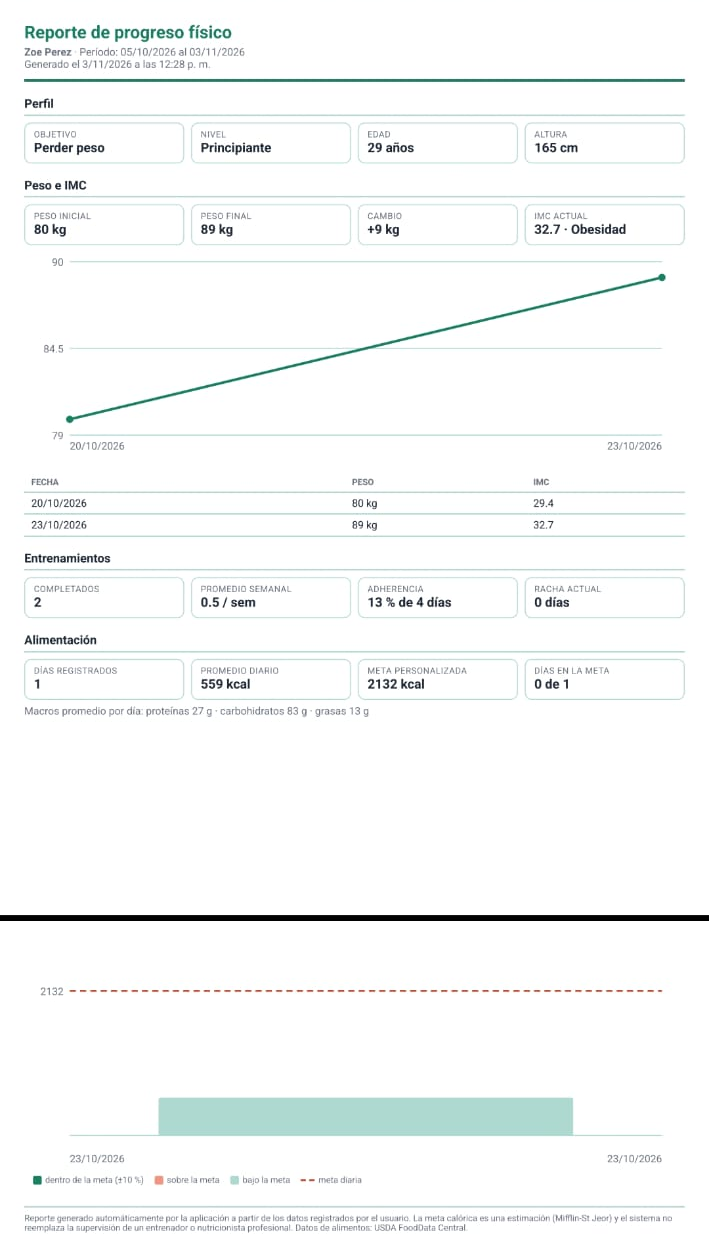
\includegraphics[height=0.36\textheight,keepaspectratio]{figuras/reporte-progreso-pdf.png}}
    \caption{Reporte de progreso físico en PDF generado en el dispositivo de prueba}
    \label{fig:reporte-pdf}
    \fuente{Elaboración propia. Captura de pantalla del reporte generado por la
    aplicación en el Infinix HOT 50 Pro+ (3 de noviembre de 2026).}
\end{figure}

A continuación, se describe la \emph{Story Card} del reporte de progreso en PDF:

\begin{table}[H]
\centering
\small
\renewcommand{\arraystretch}{1.2}

\begin{tabularx}{\textwidth}{|Y|Y|Y|}
\hline
\rowcolor{encabezado}
\textbf{Story Card} & \textbf{Nombre del proyecto} & \textbf{Estimación} \\
\hline
13 & CoachApp & Por completar \\
\hline

\multicolumn{2}{|l|}{\textbf{Nombre.} Reporte de progreso en PDF}
& \textbf{Fecha.} Por completar \\
\hline

\multicolumn{3}{|l|}{\textbf{Descripción}} \\
\hline
\multicolumn{3}{|p{\dimexpr\textwidth-2\tabcolsep-2\arrayrulewidth\relax}|}{%
El usuario genera un reporte de su progreso en PDF para guardarlo o
compartirlo.
} \\
\hline

\multicolumn{3}{|l|}{\textbf{Prueba de aceptación}} \\
\hline

\multicolumn{3}{|p{\dimexpr\textwidth-2\tabcolsep-2\arrayrulewidth\relax}|}{%
Generar el reporte eligiendo el período (7, 30, 90 días o todo el historial) y
comprobar que el PDF incluye perfil, peso e IMC, entrenamientos y
alimentación, y que se abre la hoja de compartir del sistema.
} \\
\hline

\multicolumn{2}{|l|}{\textbf{Excepciones}}
& \textbf{Riesgo.} Por evaluar \\
\hline

\multicolumn{3}{|p{\dimexpr\textwidth-2\tabcolsep-2\arrayrulewidth\relax}|}{%
Sin excepciones definidas.
} \\
\hline

\end{tabularx}
\caption{Story Card 13: Reporte de progreso en PDF}
\label{tab:hu-it6-reporte}
\fuente{Elaboración propia.}
\end{table}

\subsubsection{Pantalla de inicio}

En esta pantalla se puede observar la pantalla principal de la aplicación, que
saluda al usuario por su nombre. La tarjeta \emph{Hoy} presenta el día de la
rutina activa con su enfoque y el número de ejercicios, junto con los botones
para empezar el día y ver sus detalles. La sección \emph{Esta semana} muestra
la racha y los días completados de la semana, y el acceso \emph{Escanear
máquina} abre el escáner para identificar una máquina con la cámara
(Figura~\ref{fig:cap-inicio}).

\captura{inicio}{Pantalla de inicio}{fig:cap-inicio}

A continuación, se describe la \emph{Story Card} de la pantalla de inicio:

\begin{table}[H]
\centering
\small
\renewcommand{\arraystretch}{1.2}

\begin{tabularx}{\textwidth}{|Y|Y|Y|}
\hline
\rowcolor{encabezado}
\textbf{Story Card} & \textbf{Nombre del proyecto} & \textbf{Estimación} \\
\hline
14 & CoachApp & Por completar \\
\hline

\multicolumn{2}{|l|}{\textbf{Nombre.} Pantalla de inicio}
& \textbf{Fecha.} Por completar \\
\hline

\multicolumn{3}{|l|}{\textbf{Descripción}} \\
\hline
\multicolumn{3}{|p{\dimexpr\textwidth-2\tabcolsep-2\arrayrulewidth\relax}|}{%
El usuario ve en el inicio un resumen de su rutina activa y de sus registros.
} \\
\hline

\multicolumn{3}{|l|}{\textbf{Prueba de aceptación}} \\
\hline

\multicolumn{3}{|p{\dimexpr\textwidth-2\tabcolsep-2\arrayrulewidth\relax}|}{%
Abrir el inicio y comprobar que muestra la rutina activa, su número de
ejercicios y días por semana, y el número real de registros de peso.
} \\
\hline

\multicolumn{2}{|l|}{\textbf{Excepciones}}
& \textbf{Riesgo.} Por evaluar \\
\hline

\multicolumn{3}{|p{\dimexpr\textwidth-2\tabcolsep-2\arrayrulewidth\relax}|}{%
Sin excepciones definidas.
} \\
\hline

\end{tabularx}
\caption{Story Card 14: Pantalla de inicio}
\label{tab:hu-it6-inicio}
\fuente{Elaboración propia.}
\end{table}

\subsubsection{Codificación}

\paragraph{Registro del progreso.} \archivo{ProgressController} valida el
peso (entre 10 y 500~kg), la estatura opcional y unas notas de hasta 500
caracteres; si hay estatura, calcula el IMC reutilizando
\archivo{bmiCalculator}, y guarda el registro en
\archivo{usuarios/\{uid\}/progresoFisico}. Para evitar que el usuario
reescriba su estatura, la pantalla la precarga desde el perfil.

\paragraph{Visualización del progreso.} La vista \emph{Cuerpo} presenta los
últimos ocho registros en un gráfico de peso o IMC, la variación respecto al
primer registro, la categoría de IMC actual y el historial de mediciones.
Estos indicadores se calculan a partir de los registros observados en tiempo
real, sin crear una colección adicional de reportes.

\paragraph{Reporte personalizado en PDF.} El usuario puede generar un reporte
de 7, 30 o 90 días, o de todo su historial. \archivo{ReportsController}
reúne los datos; \archivo{progressReport.ts} calcula el resumen y construye
el HTML; y \archivo{pdfService.ts} genera y comparte el PDF mediante
\archivo{expo-print} y \archivo{expo-sharing}. El documento incluye perfil,
peso e IMC, entrenamientos y alimentación
(Figura~\ref{fig:reporte-pdf}). La comprobación en el dispositivo de prueba se
documenta en la sección~\ref{sec:des-pruebas}.

\paragraph{Seguimiento de entrenamientos.} El usuario marca los días
completados de su rutina. \archivo{WorkoutsController} registra cada
entrenamiento con la fecha local como identificador, lo que evita duplicar
el registro del mismo día. A partir de esas fechas se calculan la racha,
los días entrenados en la semana y el total acumulado. La racha se cuenta
desde ayer si el entrenamiento de hoy aún no se ha completado, para mantenerla
vigente durante el día (Código~\ref{lst:racha}).

\begin{lstlisting}[language=TypeScript, caption={Cálculo de la racha de entrenamientos}, label={lst:racha}]
export function calcularRacha(
  fechasCompletadas: ReadonlySet<string>, ahora: Date,
): number {
  const cursor = inicioDelDia(ahora);
  // Si hoy aun no se completo, la racha se evalua desde ayer.
  if (!fechasCompletadas.has(formatearFechaISO(cursor))) {
    cursor.setDate(cursor.getDate() - 1);
  }
  let racha = 0;
  while (fechasCompletadas.has(formatearFechaISO(cursor))) {
    racha++;
    cursor.setDate(cursor.getDate() - 1);
  }
  return racha;
}
\end{lstlisting}


% =====================================================================
% MEJORADO (27 oct 2026): integración #5-#7, métricas de código, verificación y suites de pruebas.
\subsection{Fase de estabilización}
\label{sec:des-estabilizacion}

En esta fase se concentró el trabajo en integrar los módulos, uniformar la
arquitectura y verificar la calidad del código. Las adiciones funcionales
corresponden al componente de servidor (funciones \archivo{buscarAlimentos} y
\archivo{guardarRutina}), que se incorporó para proteger la clave de la API de
nutrición y para validar en el servidor la creación de rutinas, y, el 3 de
noviembre de 2026, al reconocimiento de máquinas en la nube
(\archivo{reconocerMaquina}) y al módulo nativo de ARCore
(sección~\ref{sec:des-produccion}).

\subsubsection{Integración de los módulos}

Los módulos desarrollados en las ramas \archivo{feature/auth},
\archivo{feature/machines} y \archivo{feature/ejercicios} se integraron en
\archivo{develop} mediante las solicitudes de integración \#1, \#3 y \#4. Los
módulos de rutinas, escáner, nutrición y progreso se desarrollaron en
\archivo{feature/routines}, integrada mediante la solicitud \#5 (18 de octubre
de 2026). La solicitud \#6 (19 de octubre) incorporó el cambio de nombre de los
archivos a nombres en inglés (\archivo{refactor/english-file-names}) y la
solicitud \#7 (27 de octubre) integró la rama \archivo{feature/modelAI}, con los
modelos de TensorFlow Lite, el componente de servidor y las pruebas de
seguridad. La navegación principal quedó unificada en la barra
de pestañas de \archivo{(app)} (Inicio, Máquinas, Progreso y Nutrición), con
las rutinas y el perfil accesibles desde el inicio, y la protección de rutas
centralizada en el diseño raíz.

\subsubsection{Refactorización por capas}

Durante las primeras iteraciones, solo el módulo de nutrición cumplía
completamente la separación en capas; las pantallas de autenticación, de
máquinas y de rutinas llamaban a Firebase directamente. En la estabilización
se extendió el patrón a todo el sistema, de modo que cada módulo cuenta con su
controlador, sus entidades, su esquema de validación y su repositorio
(Tabla~\ref{tab:modulos-capas}).

\begin{table}[H]
\centering
\caption{Componentes de cada módulo por capa}
\label{tab:modulos-capas}
\small
\begin{tabularx}{\textwidth}{|L{2.4cm}|L{4.5cm}|Y|L{2.7cm}|}
\hline
\rowcolor{encabezado} \textbf{Módulo} & \textbf{Controlador} & \textbf{Modelo (entidad /
repositorio)} & \textbf{Vista} \\
\hline
Autenticación & \archivo{AuthController} & \archivo{Usuario} /
\archivo{userRepository} & \archivo{(auth)}, \archivo{(onboarding)},
\archivo{profile} \\ \hline
Máquinas & \archivo{MachinesController} & \archivo{Maquina} /
\archivo{machineRepository} & \archivo{machines/*} \\ \hline
Ejercicios & \archivo{ExercisesController}, \archivo{WgerExercisesController} &
\archivo{Ejercicio}, \archivo{EjercicioWger} / repositorios de ejercicios &
Modales de selección \\ \hline
Rutinas & \archivo{RoutinesController} & \archivo{Rutina} /
\archivo{routineRepository} & \archivo{routines/*} \\ \hline
Nutrición & \archivo{NutritionController} & \archivo{RegistroNutricional},
\archivo{AlimentoUSDA} / \archivo{nutritionRepository},
\archivo{foodRepository} & \archivo{nutrition} \\ \hline
Progreso & \archivo{ProgressController} & \archivo{ProgresoFisico} /
\archivo{progressRepository} & \archivo{progress/*}, inicio \\ \hline
Entrenamientos & \archivo{WorkoutsController} & \archivo{Entrenamiento}
/ \archivo{workoutRepository} & \archivo{progress/*} \\
\hline
\end{tabularx}
\end{table}

Otras mejoras aplicadas en la refactorización fueron:

\begin{itemize}
    \item \textbf{Tiempo real en lugar de recarga manual.} Las pantallas que
    consultaban los datos una sola vez y ofrecían una función de recarga
    pasaron a suscribirse con \archivo{onSnapshot} a través de los métodos
    \archivo{observar} de cada controlador, con la cancelación de la
    suscripción al desmontar la pantalla.
    \item \textbf{Manejo de errores de las suscripciones.} Se añadió un
    manejador por defecto que, ante un error de lectura, registra un aviso y
    entrega un resultado vacío para que la interfaz no quede esperando
    indefinidamente. El error de permisos que se produce al cerrar sesión con
    suscripciones activas se reconoce como esperado y se ignora.
    \item \textbf{Limpieza de campos indefinidos.} Firestore rechaza los
    campos con valor \archivo{undefined}; en lugar de exigir que cada
    repositorio lo tenga en cuenta, la limpieza se centralizó en
    \archivo{firestoreService}, el único archivo que usa el SDK.
    \item \textbf{Validación en el controlador.} Todas las operaciones de
    escritura validan sus datos con Zod antes de llegar al repositorio, y las
    reglas de seguridad repiten las validaciones críticas en el servidor.
    \item \textbf{Reglas alineadas con el modelo real.} Las reglas de
    Firestore se revisaron campo por campo contra las entidades y los
    repositorios, de modo que cada escritura que realiza la aplicación
    satisface su regla y ninguna otra es aceptada.
    \item \textbf{Convenciones de código.} Importaciones con el alias
    \archivo{@/} en lugar de rutas relativas largas, formato uniforme con
    Prettier y reglas de análisis estático de React (incluidas las de
    \emph{hooks}) sin desactivar.
\end{itemize}

\subsubsection{Métricas del código}

La Tabla~\ref{tab:metricas} resume el tamaño del código fuente por capa al
cierre de la estabilización.

\begin{table}[H]
\centering
\caption{Tamaño del código fuente por capa}
\label{tab:metricas}
\begin{tabular}{|L{3.0cm}|L{5.4cm}|C{1.8cm}|C{1.8cm}|}
\hline
\rowcolor{encabezado} \textbf{Capa} & \textbf{Carpetas} & \textbf{Archivos} & \textbf{Líneas} \\
\hline
Vista & \archivo{app/}, \archivo{components/} & 87 & 11\,410 \\ \hline
Controlador & \archivo{controllers/}, \archivo{utils/}, \archivo{store/},
\archivo{hooks/} & 41 & 5\,454 \\ \hline
Modelo & \archivo{models/}, \archivo{schemas/} & 32 & 1\,852 \\ \hline
Servicios & \archivo{services/}, \archivo{config/} & 20 & 1\,423 \\ \hline
Otros & \archivo{constants/}, \archivo{types/} & 6 & 93 \\
\hline
\textbf{Total} & & \textbf{186} & \textbf{20\,232} \\
\hline
\end{tabular}
\fuente{Conteo de archivos \archivo{.ts} y \archivo{.tsx} de la carpeta
\archivo{src/}, sin las pruebas automáticas, incluidos comentarios y líneas en
blanco, al 3 de noviembre de 2026. No incluye el código de las funciones de
servidor (\archivo{functions/}) ni el del módulo nativo de ARCore
(\archivo{modules/coach-ar/}, 606 líneas de Kotlin en cuatro archivos). El
crecimiento respecto del 27 de octubre se debe sobre todo a los componentes
compartidos de interfaz, a los servicios y esquemas del reconocimiento en la
nube y a la interfaz tipada de la vista de realidad aumentada.}
\end{table}

\subsubsection{Verificación estática}

Como criterio de cierre de la fase se estableció una secuencia de
verificaciones automáticas que el código debe superar
(Tabla~\ref{tab:verificacion-estatica}).

\begin{table}[H]
\centering
\caption{Verificaciones estáticas del código}
\label{tab:verificacion-estatica}
\begin{tabularx}{\textwidth}{|L{4.0cm}|Y|L{3.4cm}|}
\hline
\rowcolor{encabezado} \textbf{Verificación} & \textbf{Qué detecta} & \textbf{Resultado} \\
\hline
\archivo{tsc --noEmit} & Errores de tipos en todo el proyecto (TypeScript
estricto). & Sin errores (registro del proyecto del 3 de noviembre de 2026) \\ \hline
\archivo{eslint .} & Errores y malas prácticas, incluidas las reglas de
\emph{hooks} de React. & Sin errores (registro del 3 de noviembre de 2026) \\ \hline
\archivo{prettier --check} & Formato no uniforme del código. &
Conforme (registro del 3 de noviembre de 2026) \\
\hline
\end{tabularx}
\end{table}

\subsubsection{Pruebas unitarias automáticas}
\label{sec:estab-jest}

Como complemento de la verificación estática, se configuró Jest con el
\emph{preset} \archivo{jest-expo} y se escribieron pruebas para la lógica pura
del sistema, es decir, las funciones que no dependen de Firebase ni de módulos
nativos. Se ejecutan con \archivo{npm test}. La
Tabla~\ref{tab:suites-jest} lista los archivos de prueba de la aplicación, que
son 20 y comprenden 160 casos; en la ejecución del 3 de noviembre de 2026 todos
resultaron aprobados, igual que los 22 casos de las funciones del servidor y las
5 pruebas de JVM del módulo de ARCore (registro del proyecto en
\archivo{docs/ARCORE.md}). Su detalle se presenta en la
sección~\ref{sec:pruebas-unitarias}. \pendiente{conservar la salida de
\texttt{npm test} como evidencia para el tribunal.}

\begin{table}[H]
\centering
\caption{Suites de pruebas unitarias}
\label{tab:suites-jest}
\small
\begin{tabularx}{\textwidth}{|L{5.0cm}|Y|}
\hline
\rowcolor{encabezado} \textbf{Suite} & \textbf{Qué verifica} \\
\hline
\archivo{bmiCalculator} & Cálculo del IMC, límites de las categorías de la
OMS y mensajes. \\ \hline
\archivo{nutritionGoals} & Ecuación de Mifflin-St Jeor, factores de actividad,
ajuste por objetivo, piso calórico y coherencia de los macronutrientes. \\ \hline
\archivo{workoutStats} & Fechas, racha, semana y total de entrenamientos. \\ \hline
\archivo{workoutSession} & Creación de la sesión, series completadas y
descansos. \\ \hline
\archivo{routineGenerator} & Orden de las plantillas y esquemas (contrato con el
modelo), reglas de \archivo{decidirClases} y reparto de ejercicios. \\ \hline
\archivo{features} & Vector de entrada del modelo de rutinas y valores por
defecto. \\ \hline
\archivo{tfliteService} & Carga diferida del intérprete de TensorFlow Lite. \\ \hline
\archivo{ProgressController}, \archivo{ReportsController} & Actualización
parcial del progreso y cálculo de los reportes. \\ \hline
\archivo{MachinesController}, \archivo{machineRecognition} & Candidatas con su
caja, que no se mezclan con las de otras máquinas; preparación del objetivo de
ARCore y esquema de la respuesta del reconocimiento. \\ \hline
\archivo{workoutSessionStorage} & Persistencia de la sesión de entrenamiento
guiada. \\ \hline
\archivo{exerciseDbRepository}, \archivo{wgerImageRepository},
\archivo{localDemonstrationRepository} & Repositorios de ejercicios y
demostraciones locales por máquina. \\ \hline
\archivo{persisted} & Esquemas de los datos persistidos. \\ \hline
\archivo{environment}, \archivo{loadingProgress}, \archivo{typography} &
Variables de entorno faltantes, porcentaje de carga simulado y selección de
fuentes por peso. \\
\hline
\end{tabularx}
\fuente{Carpetas \archivo{\_\_tests\_\_} de \archivo{src/}. Las pruebas del
componente de servidor y de las reglas de seguridad se describen en la
sección~\ref{sec:pruebas-seguridad}.}
\end{table}

\newcommand{\pendcorto}{\textcolor{red!70!black}{\textbf{[PEND.]}}}
% =====================================================================
% MEJORADO (27 oct 2026): pruebas de seguridad (reglas y funciones), umbral de reconocimiento,
% Android 7.0 (API 24) y tabla de desviaciones.
\section{Prueba final}
\label{sec:des-pruebas}

La última fase de Mobile-D verifica que el producto cumpla sus
requerimientos. Las pruebas se organizaron en seis niveles, de los más
automáticos a los que requieren al usuario (Tabla~\ref{tab:estrategia}).

\begin{table}[H]
\centering
\caption{Estrategia de pruebas}
\label{tab:estrategia}
\begin{tabularx}{\textwidth}{|L{3.5cm}|Y|L{3.4cm}|}
\hline
\rowcolor{encabezado} \textbf{Nivel} & \textbf{Objeto de la prueba} & \textbf{Técnica} \\
\hline
Verificación estática & Tipos y calidad de todo el código. & Compilador y
analizadores (sección~\ref{sec:des-estabilizacion}) \\ \hline
Lógica de negocio & Funciones puras: generador de rutinas, IMC, estadísticas
de entrenamiento, porciones de alimentos y traducción de consultas. &
Pruebas unitarias con valores límite \\ \hline
Reglas de seguridad y funciones & Aislamiento entre usuarios, validación de
datos y control de acceso en el servidor. & Escenarios permitidos y denegados
(emulador de Firebase) \\ \hline
Funcionales & Cada requerimiento funcional en la aplicación instalada. &
Caja negra, casos de prueba \\ \hline
Usabilidad & Facilidad de uso de las tareas principales. & Tareas con
usuarios \\ \hline
Aceptación & Cumplimiento de cada objetivo específico. & Trazabilidad
objetivo--requerimiento--prueba \\
\hline
\end{tabularx}
\end{table}

\subsection{Verificación técnica}

\subsubsection{Pruebas de la lógica de negocio}
\label{subsec:pruebas-logica}

Las funciones de las reglas de negocio no dependen de la red ni de la base de
datos, por lo que se ejercitaron directamente con Node.js~22 sobre el código
fuente del proyecto, sin modificar su lógica. Las funciones del controlador de
nutrición se copiaron textualmente a un archivo auxiliar para aislarlas del SDK
de Firebase. La ejecución se realizó el 14 de octubre de 2026.

\paragraph{Generador de rutinas.} Se evaluaron las doce combinaciones posibles
de objetivo y nivel. La Tabla~\ref{tab:prueba-generador} muestra los
resultados obtenidos, que coinciden en todos los casos con las reglas de las
Tablas~\ref{tab:reglas-frecuencia} a~\ref{tab:reglas-division}.

\begin{table}[H]
\centering
\caption{Resultados del generador para las doce combinaciones de entrada}
\label{tab:prueba-generador}
\small
\begin{tabular}{|L{2.5cm}|L{2.2cm}|C{0.9cm}|C{1.9cm}|L{4.4cm}|C{1.1cm}|}
\hline
\rowcolor{encabezado} \textbf{Objetivo} & \textbf{Nivel} & \textbf{Días} & \textbf{Series × Rep.
(desc.)} & \textbf{División obtenida} & \textbf{Ejerc.} \\
\hline
Ganar masa & Principiante & 3 & 4×9 (90 s) & Emp. -- Tir. -- Pie. & 15 \\ \hline
Ganar masa & Intermedio & 4 & 4×9 (90 s) & Emp. -- Tir. -- Pie. -- C.C. & 21 \\ \hline
Ganar masa & Avanzado & 5 & 4×9 (90 s) & Emp. -- Tir. -- Pie. -- Emp. -- Tir. & 25 \\ \hline
Mantenimiento & Principiante & 3 & 3×12 (60 s) & Emp. -- Tir. -- Pie. & 15 \\ \hline
Mantenimiento & Intermedio & 4 & 3×12 (60 s) & Emp. -- Tir. -- Pie. -- C.C. & 21 \\ \hline
Mantenimiento & Avanzado & 5 & 3×12 (60 s) & Emp. -- Tir. -- Pie. -- Emp. -- Tir. & 25 \\ \hline
Perder peso & Principiante & 3 & 3×15 (45 s) & Emp. -- Car. -- Pie. & 14 \\ \hline
Perder peso & Intermedio & 4 & 3×15 (45 s) & Emp. -- Tir. -- Car. -- Pie. & 19 \\ \hline
Perder peso & Avanzado & 5 & 3×15 (45 s) & Emp. -- Tir. -- Pie. -- Car. -- C.C. & 25 \\ \hline
Resistencia & Principiante & 3 & 3×18 (30 s) & Emp. -- Car. -- Pie. & 14 \\ \hline
Resistencia & Intermedio & 4 & 3×18 (30 s) & Emp. -- Tir. -- Car. -- Pie. & 19 \\ \hline
Resistencia & Avanzado & 5 & 3×18 (30 s) & Emp. -- Tir. -- Pie. -- Car. -- C.C. & 25 \\
\hline
\end{tabular}
\fuente{Ejecución de \archivo{generarPlanHeuristico} (comportamiento base, sin
edad, IMC ni días disponibles). Emp.: empuje; Tir.:
tirón; Pie.: pierna; Car.: cardio; C.C.: cuerpo completo; Ejerc.: total de
ejercicios por semana.}
\end{table}

\paragraph{Cálculo del IMC.} Se probaron valores en los límites de cada
categoría de la OMS (Tabla~\ref{tab:prueba-imc}). Todos los casos produjeron
el resultado esperado.

\begin{table}[H]
\centering
\caption{Pruebas de valores límite del cálculo y la clasificación del IMC}
\label{tab:prueba-imc}
\small
\begin{tabular}{|C{2.2cm}|C{2.4cm}|C{2.2cm}|L{3.3cm}|C{2cm}|}
\hline
\rowcolor{encabezado} \textbf{Peso (kg)} & \textbf{Estatura (cm)} & \textbf{IMC} &
\textbf{Categoría obtenida} & \textbf{Resultado} \\
\hline
50.0 & 170 & 17.3 & Bajo peso & Correcto \\ \hline
53.4 & 170 & 18.5 & Normal & Correcto \\ \hline
70.0 & 175 & 22.9 & Normal & Correcto \\ \hline
72.2 & 170 & 25.0 & Sobrepeso & Correcto \\ \hline
86.7 & 170 & 30.0 & Obesidad & Correcto \\ \hline
100.0 & 170 & 34.6 & Obesidad & Correcto \\ \hline
\multicolumn{3}{|c|}{Clasificación de 18.4 / 18.5} & Bajo peso / Normal & Correcto \\ \hline
\multicolumn{3}{|c|}{Clasificación de 24.9 / 25.0} & Normal / Sobrepeso & Correcto \\ \hline
\multicolumn{3}{|c|}{Clasificación de 29.9 / 30.0} & Sobrepeso / Obesidad & Correcto \\
\hline
\end{tabular}
\fuente{Ejecución de \archivo{calcularIMC} y \archivo{clasificarIMC}.}
\end{table}

\paragraph{Reparto, entrenamientos, porciones y traducción.} La
Tabla~\ref{tab:prueba-otras} reúne las demás pruebas de funciones puras. Para
las estadísticas de entrenamiento se fijó la fecha actual en el miércoles 14 de
octubre de 2026.

\begin{table}[H]
\centering
\caption{Otras pruebas de la lógica de negocio}
\label{tab:prueba-otras}
\footnotesize
\begin{tabularx}{\textwidth}{|L{1.1cm}|L{4.1cm}|Y|Y|}
\hline
\rowcolor{encabezado} \textbf{ID} & \textbf{Función} & \textbf{Entrada} & \textbf{Resultado obtenido} \\
\hline
PL-01 & \archivo{repartirCantidad} & 5 ejercicios en 3 categorías & 2 -- 2 -- 1 \\ \hline
PL-02 & \archivo{repartirCantidad} & 6 ejercicios en 3 categorías & 2 -- 2 -- 2 \\ \hline
PL-03 & \archivo{repartirCantidad} & 4 ejercicios en 2 categorías & 2 -- 2 \\ \hline
PL-04 & Estadísticas de entrenamiento & Días 12, 13 y 14 de octubre (hoy
incluido) & Racha 3; semana 3; total 3 \\ \hline
PL-05 & Estadísticas de entrenamiento & Días 12 y 13 (hoy sin completar) &
Racha 2; semana 2 \\ \hline
PL-06 & Estadísticas de entrenamiento & Días 10 y 12 (falta el día 13) &
Racha 0; semana 1 \\ \hline
PL-07 & Estadísticas de entrenamiento & Diez días consecutivos hasta hoy &
Racha 10; semana 3; total 10 \\ \hline
PL-08 & Estadísticas de entrenamiento & Sin registros & Racha 0; semana 0;
total 0 \\ \hline
PL-09 & \archivo{calcularPorcion} & Arroz (130~kcal, 2.7~g P, 28~g C, 0.3~g
G por 100~g), 200~g & 260~kcal; 5.4~g P; 56~g C; 0.6~g G \\ \hline
PL-10 & \archivo{calcularPorcion} & Pollo (165~kcal, 31~g P por 100~g), 150~g
& 248~kcal; 46.5~g P; 0~g C; 5.4~g G \\ \hline
PL-11 & \archivo{calcularPorcion} & Cualquier alimento, 0~g & Todos los
valores en 0 \\ \hline
PL-12 & \archivo{calcularResumenDiario} & Dos alimentos de hoy (arroz y pollo),
uno de otra fecha y un cálculo de IMC & Solo suma los dos de hoy: 508~kcal,
quedan 1\,492; 25.4\,\% de la meta de referencia (2\,000~kcal) \\ \hline
PL-13 & \archivo{calcularResumenDiario} & Un alimento de 2\,600~kcal & Porcentaje
limitado a 100\,\%; restantes 0 \\ \hline
PL-14 & \archivo{traducirConsulta} & ``pechuga de pollo'', ``Plátano'',
``leche descremada'' & ``chicken breast'', ``banana'', ``milk nonfat'' \\ \hline
PL-15 & \archivo{traducirConsulta} & ``chicken'' y ``a'' & ``chicken'' sin
cambio; ``a'' no genera consulta \\
\hline
\end{tabularx}
\end{table}

\subsubsection{Pruebas unitarias automáticas}
\label{sec:pruebas-unitarias}

Las pruebas anteriores se ejecutaron una vez, con \emph{scripts} auxiliares.
Para que las reglas de negocio puedan verificarse de forma repetible después de
cada cambio, se escribieron 20 archivos de prueba de Jest
(Tabla~\ref{tab:suites-jest}), que se ejecutan con \archivo{npm test}. Las
funciones probadas son puras, por lo que las pruebas no requieren Firebase ni
un dispositivo. Entre los casos cubiertos están:

\begin{itemize}
    \item \textbf{IMC:} los límites exactos de cada categoría de la OMS
    (18,4 es bajo peso; 18,5 es normal; 24,9 es normal; 25 es sobrepeso; 30 es
    obesidad).
    \item \textbf{Metas nutricionales:} que un hombre de 25 años, 75~kg y
    178~cm, que entrena cuatro días para ganar masa, obtenga una tasa basal de
    1\,743~kcal y una meta de 3\,001~kcal; que perder peso aplique un déficit de
    500~kcal; que nunca se baje del piso calórico (1\,200~kcal para mujeres y
    1\,500~kcal para hombres); y que los macronutrientes no sean negativos y
    reconstruyan las calorías con una tolerancia de 10~kcal.
    \item \textbf{Generador de rutinas:} que el orden de las seis plantillas y
    de los cuatro esquemas coincida con el del \emph{script} de entrenamiento
    del modelo (si cambiara, el modelo dejaría de ser válido); que IMC $\geq$ 30
    active el énfasis en cardio; que los mayores de 60 años no reciban
    hipertrofia ni esquema metabólico y los menores de 16 no reciban
    hipertrofia; y que cualquier combinación de perfil produzca clases
    válidas.
    \item \textbf{Vector de entrada del modelo:} el orden de las diez
    características, la codificación \emph{one-hot} del objetivo y los valores
    por defecto cuando faltan datos del perfil.
    \item \textbf{Estadísticas y sesión de entrenamiento:} racha, semana y
    total; creación de la sesión, series completadas y descansos.
    \item \textbf{Reconocimiento y realidad aumentada:} que las cajas de las
    candidatas alternativas no se mezclen con las de la máquina principal, que
    el objetivo que recibe la vista de ARCore tome la caja de la candidata
    confirmada, y que el esquema de la respuesta rechace cajas inválidas.
    \item \textbf{Otros componentes:} carga diferida de TensorFlow Lite,
    esquemas de los datos persistidos, actualización parcial del progreso,
    persistencia de la sesión de entrenamiento, demostraciones locales por
    máquina y verificación de las variables de entorno.
\end{itemize}

\subsubsection{Pruebas de las reglas de seguridad y de las funciones del servidor}
\label{sec:pruebas-seguridad}

Las reglas de seguridad y las funciones del servidor constituyen la barrera
frente a un acceso malintencionado, porque las credenciales de Firebase están
contenidas en la aplicación y no son secretas; App Check añade una verificación
complementaria de la procedencia de las solicitudes. La Tabla~\ref{tab:prueba-reglas} define los escenarios evaluados
y el resultado que exigen las reglas del Anexo~\ref{anx:reglas}. Los
escenarios se automatizaron con el emulador de Firebase (comando
\archivo{npm run test:security}), autenticando como un usuario $A$ y operando
sobre datos propios o de otro usuario $B$: el archivo
\archivo{tests/security/rules.test.mjs} declara 11 pruebas sobre Firestore y
Storage, y \archivo{functions/test/security.integration.mjs} declara 4 pruebas
de integración de las funciones. Las pruebas de los esquemas del servidor
(\archivo{npm run test:backend}), que incluyen la interpretación de la
respuesta del reconocimiento (clases, equivalencias, cajas inválidas y confianza
fuera de rango), se ejecutaron el 3 de noviembre de 2026 y aprobaron 22 de 22
casos. Los 19 escenarios de seguridad de la
Tabla~\ref{tab:prueba-reglas} también se completaron satisfactoriamente: los
resultados obtenidos coincidieron con los esperados.

\begin{table}[H]
\centering
\caption{Escenarios de prueba de las reglas de seguridad}
\label{tab:prueba-reglas}
\footnotesize
\begin{tabularx}{\textwidth}{|L{1.3cm}|Y|C{1.8cm}|C{1.9cm}|}
\hline
\rowcolor{encabezado} \textbf{ID} & \textbf{Escenario} & \textbf{Esperado} & \textbf{Obtenido} \\
\hline
SEG-01 & Usuario no autenticado lee \archivo{maquinas/\{id\}} & Denegado & Denegado \\ \hline
SEG-02 & $A$ lee \archivo{maquinas/\{id\}} & Permitido & Permitido \\ \hline
SEG-03 & $A$ escribe en \archivo{maquinas/\{id\}} & Denegado & Denegado \\ \hline
SEG-04 & $A$ lee \archivo{usuarios/A/rutinas} & Permitido & Permitido \\ \hline
SEG-05 & $A$ lee \archivo{usuarios/B/rutinas} & Denegado & Denegado \\ \hline
SEG-06 & $A$ envía a \archivo{guardarRutina} una rutina con
\archivo{diasPorSemana = 8} & Rechazado & Rechazado \\ \hline
SEG-07 & $A$ envía a \archivo{guardarRutina} una rutina con
\archivo{usuarioId = B} (el propietario se toma de la identidad autenticada) & Rechazado & Rechazado \\ \hline
SEG-08 & $A$ modifica el campo \archivo{email} de su perfil & Denegado & Denegado \\ \hline
SEG-09 & $A$ crea su perfil con \archivo{edad = 10} & Denegado & Denegado \\ \hline
SEG-10 & $A$ registra progreso con \archivo{peso = 0} & Denegado & Denegado \\ \hline
SEG-11 & $A$ registra ingesta con \archivo{calorias = -100} & Denegado & Denegado \\ \hline
SEG-12 & $A$ crea un entrenamiento cuyo \archivo{fecha} difiere del
identificador del documento & Denegado & Denegado \\ \hline
SEG-13 & $A$ crea un entrenamiento con \archivo{dia = 8} & Denegado & Denegado \\ \hline
SEG-14 & $A$ crea su perfil con \archivo{creadoEn} distinto de la hora del
servidor & Denegado & Denegado \\ \hline
SEG-15 & $A$ sube un archivo a Storage & Denegado & Denegado \\ \hline
SEG-16 & $A$ crea directamente un documento en \archivo{usuarios/A/rutinas},
sin usar la función & Denegado & Denegado \\ \hline
SEG-17 & Llamada a \archivo{guardarRutina}, \archivo{buscarAlimentos} o
\archivo{reconocerMaquina} sin autenticación & Rechazado & Rechazado \\ \hline
SEG-18 & Llamada a las funciones con un usuario anónimo & Rechazado & Rechazado \\ \hline
SEG-19 & Solicitudes concurrentes que superan la cuota por usuario & Limitadas a la cuota & Limitadas a la cuota \\
\hline
\end{tabularx}
\end{table}

\subsubsection{Evaluación de los modelos de inteligencia artificial}
\label{sec:pruebas-ia}

La evaluación distingue el clasificador local, el detector en la nube y el
recomendador de rutinas. Se presentan sus resultados, las condiciones de
evaluación y las limitaciones. Los resultados proceden de los registros
citados en cada tabla; no equivalen a una validación con usuarios.

\paragraph{Evaluación del clasificador local de máquinas}

\paragraph{Evaluación.} Se evaluó con validación cruzada de cinco pliegues y
cuidando que las versiones aumentadas de una misma foto nunca estuvieran en
entrenamiento y validación a la vez. La Tabla~\ref{tab:metricas-reconocimiento}
resume los resultados con imágenes limpias y con el escenario de campo
simulado.

\begin{table}[H]
\centering
\caption{Exactitud del reconocimiento de máquinas (validación cruzada, 35 clases)}
\label{tab:metricas-reconocimiento}
\small
\begin{tabular}{|l|C{2.6cm}|C{2.6cm}|}
\hline
\rowcolor{encabezado} \textbf{Escenario} & \textbf{Acierto top-1} & \textbf{Acierto top-3} \\
\hline
Imágenes limpias del catálogo & 43,4\,\% & 65,9\,\% \\ \hline
Campo simulado (fondos y cámara) & 38,5\,\% & 61,4\,\% \\
\hline
\end{tabular}
\fuente{Archivo \archivo{ml/results/recognition/recognition\_metrics.json}. El
azar acertaría el 2,9\,\% (1 de 35).}
\end{table}

El umbral de confianza se calibró sobre esas mismas predicciones
(Tabla~\ref{tab:umbral-reconocimiento}): a mayor umbral, más seguro es el
reconocimiento automático, pero menos veces se usa. Se eligió 0,8 porque,
cuando la aplicación acepta la máquina sin preguntar, acierta
aproximadamente 85 de cada 100 veces; en las demás ocasiones el usuario
confirma una sugerencia ya preseleccionada.

\begin{table}[H]
\centering
\caption{Calibración del umbral de confianza}
\label{tab:umbral-reconocimiento}
\small
\begin{tabular}{|C{2.2cm}|C{3.2cm}|C{3.2cm}|}
\hline
\rowcolor{encabezado} \textbf{Umbral} & \textbf{Cobertura} & \textbf{Precisión} \\
\hline
0,5 & 44,4\,\% & 60,5\,\% \\ \hline
0,7 & 23,6\,\% & 75,1\,\% \\ \hline
\textbf{0,8} & \textbf{15,8\,\%} & \textbf{85,4\,\%} \\ \hline
0,9 & 9,2\,\% & 92,2\,\% \\
\hline
\end{tabular}
\fuente{Archivo \archivo{ml/results/recognition/recognition\_metrics.json}.
Cobertura: proporción de fotos que superan el umbral; precisión: aciertos entre
ellas.}
\end{table}

\paragraph{Limitaciones.} El resultado es modesto y debe leerse como tal. Con
solo 399 fotografías de catálogo (de una a 25 por máquina) el modelo distingue
bien las máquinas visualmente más características, como la caminadora (93\,\%
de acierto en el campo simulado) o la bicicleta estática (67\,\%), pero casi no
reconoce otras: curl de bíceps, pantorrillas, torso rotatorio, elevaciones
laterales y remo en T se acercan al 0\,\%, y dos máquinas con una sola foto no
pudieron evaluarse. Además, las fotografías de catálogo no son imágenes tomadas
en un gimnasio real. Por ello la máquina se acepta directamente solo cuando la confianza alcanza el
umbral de 0,8, con una cobertura del 15,8\,\% de las fotografías y una
precisión del 85,4\,\% en la validación cruzada; en los demás casos el
reconocimiento se presenta como una \emph{sugerencia} que el usuario confirma o
corrige. La mejora esperada proviene de
más fotografías propias o autorizadas, tomadas en gimnasios reales
(sección~\ref{sec:recomendaciones}).



\paragraph{Evolución y evaluación del detector en la nube}

\paragraph{Primera versión del detector (YOLO11x).} Esta versión parte de
YOLO11x, el tamaño extragrande de la generación YOLO11, con los pesos
preentrenados que distribuye Ultralytics (Khanam \& Hussain, 2024; Jocher
et~al., 2023). Se ajustó en Google Colab con un conjunto anotado en Roboflow
(Roboflow, Inc., s.~f.) y exportado en formato YOLO. El conjunto tiene 458
imágenes y 625 cajas de 42 clases, repartidas en 327 imágenes de entrenamiento,
88 de validación y 43 de prueba. Se entrenó durante 15 épocas con imágenes de
640$\times$640 píxeles y lotes de 16, con los aumentos de datos por defecto de
Ultralytics (mosaico, cambios de color y volteo horizontal). La evaluación se
hizo sobre la partición de prueba, en CPU, tras comprobar con \emph{hashes} que
ninguna imagen de prueba fuera idéntica a una de entrenamiento o validación
(Tabla~\ref{tab:metricas-detector}).

\begin{table}[H]
\centering
\caption{Métricas del detector de máquinas en la partición de prueba}
\label{tab:metricas-detector}
\small
\begin{tabular}{|l|C{2.6cm}|}
\hline
\rowcolor{encabezado} \textbf{Métrica} & \textbf{Valor} \\
\hline
Precisión & 79,8\,\% \\ \hline
Exhaustividad (\emph{recall}) & 29,9\,\% \\ \hline
mAP50 & 39,8\,\% \\ \hline
mAP50--95 & 37,6\,\% \\
\hline
\end{tabular}
\fuente{Archivo \archivo{ml/detection/runs/best42-evaluation/results.json},
generado con \archivo{evaluate\_best42.py}. Partición de prueba: 43 imágenes,
65 cajas, 24 clases con ejemplos; entrada de 640 píxeles; evaluación en CPU de
un computador, no en un teléfono. Definición de las métricas en Padilla
et~al. (2021).}
\end{table}

Estos resultados deben leerse con cautela por cuatro razones. La primera es que
la partición de prueba es mínima: 43 imágenes con 65 cajas, de las cuales 24
pertenecen a una sola clase (\texttt{hip\_adduction\_machine}) y 18 de las 42
clases no tienen ningún ejemplo. La segunda es el desbalance del entrenamiento:
esa misma clase aporta 91 cajas, la mediana es de 8 cajas por clase, y cuatro
clases (extensión de cuádriceps, poleas de doble cable, rack de sentadilla y
remo alto) no tienen ninguna, por lo que el detector no puede reconocerlas. La
tercera es que varias imágenes parecen series de una misma máquina vista desde
ángulos cercanos; aunque no haya duplicados exactos, la prueba puede resultar
más fácil que una situación real en un gimnasio. La cuarta es que una
exhaustividad del 29,9\,\% significa que, en el punto de operación que reporta
Ultralytics, el detector encuentra menos de un tercio de las cajas reales. Por
todo ello las cifras muestran que el procedimiento funciona de extremo a
extremo, no que el detector sea fiable en un gimnasio.

El proyecto incluye además un \emph{script} para exportar la primera versión del detector al formato
LiteRT, el sucesor de TensorFlow Lite, y ejecutarlo en el propio teléfono
(\archivo{export\_best42.py}). Está preparado, pero requiere Linux o macOS y no
se ha ejecutado ni probado en Android.

\paragraph{Versión final del detector: YOLO26m en Ultralytics Platform.} La versión
final se entrenó y se publicó en Ultralytics Platform con YOLO26 en su tamaño
mediano (m), a partir de los pesos preentrenados que distribuye Ultralytics
(Jocher et~al., 2026; Ultralytics, s.~f.-c). YOLO26 es la generación más reciente
de la familia y sus autores la orientan a dispositivos de borde, con una
inferencia que no requiere supresión de no máximos (Sapkota et~al., 2025). El
conjunto de datos (\texttt{gym-machines-data}) se creó en el editor de la
plataforma, que permite anotar con polígonos y con la ayuda de un modelo de
segmentación (SAM) (Ultralytics, s.~f.-a): cada máquina se delimitó con un
polígono y se le asignó una de las 52 clases definidas para el proyecto. La
tarea de entrenamiento es de detección, de modo que el modelo predice cajas
delimitadoras y no contornos.

Según el gráfico de distribución de clases de la plataforma, el conjunto reúne
6\,681 ejemplos anotados (Tabla~\ref{tab:distribucion-clases}). La clase más
frecuente (\texttt{prensa-piernas}) aporta 615 ejemplos, el 9,2\,\% del total,
y cinco clases tienen cuatro ejemplos o menos (\texttt{rack-sentadilla},
\texttt{press-alto}, \texttt{press-asistida}, \texttt{extension-cuadriceps} y
\texttt{remo-alto}). Las 24 clases con 100 ejemplos o más concentran el
88,9\,\% de las anotaciones, y las seis con menos de diez apenas el 0,3\,\%. El
desbalance es fuerte (de 615 ejemplos a uno en la clase más rara) y, con tan
pocos ejemplos, esas clases difícilmente pueden aprenderse o evaluarse: su
resultado individual no es interpretable y las métricas globales se apoyan
sobre todo en las clases frecuentes. Además, algunas etiquetas parecen nombrar
la misma máquina con criterios distintos (por ejemplo,
\texttt{abductores-aductores} y \texttt{hip\_adduction\_machine}, o
\texttt{curl-biceps} y \texttt{bicep\_curl\_machine}), lo que puede repartir los
ejemplos de una máquina entre dos clases.

\begin{table}[H]
\centering
\caption{Distribución de los ejemplos anotados por clase en \texttt{gym-machines-data}}
\label{tab:distribucion-clases}
\small
\begin{tabular}{|l|C{1.8cm}|C{2.2cm}|C{2.6cm}|}
\hline
\rowcolor{encabezado} \textbf{Ejemplos por clase} & \textbf{Clases} &
\textbf{Ejemplos} & \textbf{\% del total} \\
\hline
100 o más & 24 & 5\,939 & 88,9\,\% \\ \hline
De 30 a 99 & 11 & 473 & 7,1\,\% \\ \hline
De 10 a 29 & 11 & 248 & 3,7\,\% \\ \hline
Menos de 10 & 6 & 21 & 0,3\,\% \\ \hline
\textbf{Total} & \textbf{52} & \textbf{6\,681} & \textbf{100\,\%} \\
\hline
\end{tabular}
\fuente{Elaboración propia con los conteos por clase del gráfico de
distribución de clases de Ultralytics Platform.}
\end{table}

El entrenamiento duró 80 épocas, con imágenes de 640$\times$640 píxeles, lotes
de 32, una GPU, semilla 42 en modo determinista y precisión mixta automática. El
optimizador se dejó en automático y se mantuvieron los aumentos de datos por
defecto de Ultralytics (mosaico, que se desactiva en las últimas 10 épocas,
volteo horizontal, variaciones de color y borrado aleatorio). No se configuró
parada temprana (paciencia igual a 0). La corrida se registró como
\texttt{version-5} del proyecto \texttt{detect-machine}. La
Tabla~\ref{tab:metricas-detector-yolo26} resume las métricas de la última época,
calculadas sobre la partición de validación.

\begin{table}[H]
\centering
\caption{Métricas del detector final (YOLO26m) en la partición de validación}
\label{tab:metricas-detector-yolo26}
\small
\begin{tabular}{|l|C{2.6cm}|}
\hline
\rowcolor{encabezado} \textbf{Métrica} & \textbf{Valor} \\
\hline
Precisión & 57,7\,\% \\ \hline
Exhaustividad (\emph{recall}) & 45,0\,\% \\ \hline
mAP50 & 48,5\,\% \\ \hline
mAP50--95 & 44,8\,\% \\ \hline
Pérdida de caja (entrenamiento / validación) & 0,243 / 0,612 \\ \hline
Pérdida de clasificación (entrenamiento / validación) & 0,286 / 2,690 \\
\hline
\end{tabular}
\fuente{Registro de entrenamiento de Ultralytics Platform (corrida
\texttt{version-5}, época 80). Definición de las métricas en Padilla et~al.
(2021). La validación no es una partición de prueba independiente.}
\end{table}

Estas cifras son las del propio entrenamiento y deben leerse con cautela. La
partición de validación es la que Ultralytics usa también para elegir el mejor
punto de control, de modo que tiende a favorecer al modelo; no se evaluó con una
partición de prueba independiente ni con fotografías de un gimnasio real. Además,
la pérdida de clasificación en validación (2,69) es unas diez veces la de
entrenamiento (0,29), y la de caja (0,61) más del doble (0,24), lo que apunta a
sobreajuste: el modelo se ajusta bien a las imágenes que ya vio y generaliza
menos a las nuevas. Por todo ello las cifras muestran que el procedimiento
funciona de extremo a extremo, no que el detector sea fiable en un gimnasio.

\paragraph{Dispositivo utilizado para las pruebas}

\paragraph{Dispositivo de prueba.} El teléfono de prueba es un Infinix HOT 50
Pro+ (modelo X6880), un equipo de gama media cuyas características resume la
Tabla~\ref{tab:dispositivo-prueba}. Según la lista de dispositivos compatibles
de Google, este modelo admite ARCore y la API de profundidad (Google for
Developers, s.~f.-a), que es lo que necesita el módulo CoachAR. Con un único
equipo no puede afirmarse que la aplicación se comporte igual en otros
teléfonos, con cámaras, memoria o soporte de ARCore distintos.

\begin{table}[H]
\centering
\caption{Características del dispositivo de prueba}
\label{tab:dispositivo-prueba}
\small
\begin{tabular}{|l|l|}
\hline
\rowcolor{encabezado} \textbf{Característica} & \textbf{Valor} \\
\hline
Modelo & Infinix HOT 50 Pro+ (X6880) \\ \hline
Procesador & MediaTek Helio G100 \\ \hline
Memoria RAM & 8\,GB (más 5\,GB de RAM extendida) \\ \hline
Almacenamiento & 256\,GB \\ \hline
Cámara trasera & 50\,MP + 2\,MP \\ \hline
Cámara frontal & 13\,MP \\ \hline
Pantalla & 1\,080 $\times$ 2\,436 píxeles \\ \hline
Batería & 5\,000\,mAh \\ \hline
Sistema operativo & XOS 15.1.2 (basado en Android 15) \\
\hline
\end{tabular}
\fuente{Pantalla «Mi teléfono» de los ajustes del dispositivo. Compatibilidad
con ARCore: Google for Developers (s.~f.-a).}
\end{table}





\paragraph{Verificación de la realidad aumentada}

La aplicación se probó en un dispositivo físico y cumplió los criterios de
verificación de la realidad aumentada. El modelo reconoció la máquina y el
módulo \archivo{CoachAR} mostró su información mediante ARCore. El seguimiento
espacial, la consulta al servicio de reconocimiento y la visualización de la
ficha funcionaron correctamente de forma integrada. Los casos CP-42 a CP-44
del Anexo~\ref{anx:casos} se completaron satisfactoriamente.

\paragraph{Evaluación del recomendador de rutinas}

\paragraph{Resultados.} En el conjunto de prueba el modelo acertó la plantilla
en el 99,8\,\% de los casos, el esquema de carga en el 99,97\,\% y ambas a la
vez en el 99,8\,\% (Tabla~\ref{tab:metricas-rutinas}). Como comprobación
adicional se evaluó el modelo sobre una cuadrícula exhaustiva de 28\,512
perfiles que recorre todas las combinaciones de objetivo, nivel, género, días,
edades y valores de IMC alrededor de los umbrales: coincidió con las reglas en
27\,689 (97,1\,\%). Los desacuerdos se concentran justo en los umbrales, por
ejemplo con 59 años (un año antes del cambio de esquema) o con IMC de 29,9
(justo antes del énfasis cardio), donde un modelo continuo suaviza la frontera
que las reglas trazan de forma abrupta.

\begin{table}[H]
\centering
\caption{Desempeño del recomendador de rutinas sobre datos sintéticos}
\label{tab:metricas-rutinas}
\small
\begin{tabular}{|l|C{3.4cm}|}
\hline
\rowcolor{encabezado} \textbf{Medida} & \textbf{Resultado} \\
\hline
Exactitud de la plantilla semanal (prueba, 9\,000 perfiles) & 99,8\,\% \\ \hline
Exactitud del esquema de carga (prueba) & 99,97\,\% \\ \hline
Exactitud de ambas clases (prueba) & 99,8\,\% \\ \hline
Coincidencia con las reglas en la cuadrícula exhaustiva (28\,512 perfiles) &
97,1\,\% \\ \hline
Coincidencia del archivo \texttt{.tflite} con el modelo de Keras & 100\,\% \\
\hline
\end{tabular}
\fuente{Archivos \archivo{ml/results/metrics.json} y
\archivo{ml/results/model\_metadata.json}.}
\end{table}

\paragraph{Comprobación del reporte PDF}
Según el registro consignado en el documento, el 3 de noviembre de 2026 se
generó un reporte de 30 días en el Infinix HOT 50 Pro+. El archivo incluyó
perfil, peso e IMC, entrenamientos y alimentación y se abrió en el visor del
teléfono. La Figura~\ref{fig:reporte-pdf} presenta datos de demostración.
Esta comprobación corresponde al reporte y no valida el módulo de ARCore.

\subsection{Pruebas funcionales en dispositivos}

Las pruebas funcionales se realizan con la técnica de caja negra sobre el
\emph{development build} instalado en un dispositivo Android, siguiendo los
criterios de aceptación definidos en cada iteración. Se definieron 44 casos de
prueba que cubren los requerimientos funcionales RF1 a RF6; la matriz completa,
con los pasos, el resultado esperado y el resultado obtenido, se encuentra en
el Anexo~\ref{anx:casos}. La Tabla~\ref{tab:resumen-funcionales} resume su
distribución.

\begin{table}[H]
\centering
\caption{Distribución de los casos de prueba funcionales}
\label{tab:resumen-funcionales}
\begin{tabular}{|L{6cm}|C{2.5cm}|C{3.4cm}|}
\hline
\rowcolor{encabezado} \textbf{Módulo} & \textbf{Casos} & \textbf{Requerimientos} \\
\hline
Autenticación, onboarding y perfil & 9 & RF1.1 a RF1.5 \\ \hline
Guía de máquinas y ejercicios & 6 & RF2.1 a RF2.3 \\ \hline
Escáner con reconocimiento y realidad aumentada & 7 & RF2.4 \\ \hline
Rutinas y planificación & 7 & RF3.1 a RF3.3 \\ \hline
Nutrición (alimentos e IMC) & 7 & RF4.1, RF5.1 a RF5.3 \\ \hline
Progreso, entrenamientos y reportes & 8 & RF4.2, RF6.1, RF6.2 \\
\hline
\textbf{Total} & \textbf{44} & \\
\hline
\end{tabular}
\end{table}

\subsection{Pruebas funcionales con usuarios}

\subsubsection{Pruebas de usabilidad}

Las pruebas de usabilidad permitieron comprobar la realización de las tareas
principales de la aplicación (Nielsen, 1993). Las seis tareas evaluadas se
completaron correctamente y cumplieron sus criterios de éxito. La
Tabla~\ref{tab:tareas-usabilidad} presenta los resultados obtenidos.

\begin{table}[H]
\centering
\caption{Resultados de las pruebas de usabilidad}
\label{tab:tareas-usabilidad}
\small
\begin{tabularx}{\textwidth}{|L{0.7cm}|Y|Y|L{1.6cm}|}
\hline
\rowcolor{encabezado} \textbf{ID} & \textbf{Tarea} & \textbf{Criterio de éxito} & \textbf{Resultado} \\
\hline
T1 & Registrarse y completar el \emph{onboarding}. & Llega a la pantalla de
inicio. & Cumple \\ \hline
T2 & Encontrar la ficha de la prensa de piernas. & Abre la ficha desde el
catálogo. & Cumple \\ \hline
T3 & Escanear una máquina y abrir su ficha completa. & Abre la ficha desde la
superposición. & Cumple \\ \hline
T4 & Generar una rutina y marcar como completado el día de hoy. & La rutina
queda activa y el día marcado. & Cumple \\ \hline
T5 & Registrar 150~g de arroz en el diario. & El alimento aparece en la lista
del día. & Cumple \\ \hline
T6 & Registrar su peso y ver el gráfico de evolución. & Ve el nuevo punto en
el gráfico. & Cumple \\
\hline
\end{tabularx}
\end{table}

\subsection{Pruebas de aceptación por objetivo}

La Tabla~\ref{tab:trazabilidad} relaciona cada objetivo específico con los
requerimientos que lo implementan y con las pruebas que lo verifican. Esta
trazabilidad es la base de la evaluación del cumplimiento de objetivos que
realiza el tribunal (Artículo~64 del Reglamento de Titulación).

\begin{table}[H]
\centering
\caption{Trazabilidad entre objetivos, requerimientos y pruebas}
\label{tab:trazabilidad}
\small
\begin{tabularx}{\textwidth}{|L{1.1cm}|Y|L{2.2cm}|L{3.4cm}|}
\hline
\rowcolor{encabezado} \textbf{Obj.} & \textbf{Funcionalidad entregada} & \textbf{Req.} &
\textbf{Pruebas} \\
\hline
OE1 & Guía de 35 máquinas con búsqueda, filtros, fichas y escáner con
reconocimiento asistido (modelo local o detector en la nube) y ficha anclada
con ARCore en los teléfonos compatibles. & RF2.1, RF2.2, RF2.4 &
CP-10 a CP-13, CP-15 a CP-19, CP-42 a CP-44, sección~\ref{sec:pruebas-ia} \\
\hline
OE2 & Ejercicios con animación, músculo objetivo y dificultad. & RF2.3 &
CP-14 \\ \hline
OE3 & \emph{Onboarding} de objetivo, nivel y datos físicos; rutinas
generadas por un recomendador de TensorFlow Lite con respaldo de reglas. &
RF1.4, RF3.1 & CP-06 a CP-08, CP-20, CP-21,
Tabla~\ref{tab:prueba-generador}, secciones~\ref{sec:pruebas-unitarias}
y~\ref{sec:pruebas-ia} \\ \hline
OE4 & Planificador de rutinas por día, rutina activa y agregado desde la
ficha. & RF3.2, RF3.3 & CP-22 a CP-26 \\ \hline
OE5 & Diario de alimentación con calorías y macronutrientes, metas
personalizadas; calculadora de IMC con clasificación e historial. & RF4.1, RF5 &
CP-27 a CP-33, Tablas~\ref{tab:prueba-imc} y~\ref{tab:prueba-otras},
sección~\ref{sec:pruebas-unitarias} \\ \hline
OE6 & Registro de peso, estatura e IMC. & RF4.2 & CP-34, CP-35 \\ \hline
OE7 & Reporte con gráfico, variación y categoría actual; reporte en PDF por
período; seguimiento de entrenamientos con racha. & RF6 & CP-36 a CP-41,
Tabla~\ref{tab:prueba-otras} \\
\hline
\end{tabularx}
\end{table}

\subsection{Cumplimiento del alcance y desviaciones}

La Tabla~\ref{tab:desviaciones} contrasta lo planificado en los
Capítulos~\ref{cap:introduccion} y~\ref{cap:area-aplicacion} con lo que
efectivamente se entrega. Se incluye para que el alcance del producto se
evalúe con transparencia.

\begin{table}[H]
\centering
\caption{Contraste entre lo planificado y lo implementado}
\label{tab:desviaciones}
\small
\begin{tabularx}{\textwidth}{|L{3.1cm}|L{2.4cm}|Y|}
\hline
\rowcolor{encabezado} \textbf{Elemento planificado} & \textbf{Estado} & \textbf{Observación} \\
\hline
Rutinas personalizadas con IA mediante TensorFlow Lite & Completo, con
salvedad & Un modelo entrenado decide la estructura de la rutina en el
dispositivo y las reglas actúan como respaldo. Se entrenó con perfiles
sintéticos etiquetados por las reglas, por lo que imita el criterio experto y
no se validó con resultados de usuarios reales. \\ \hline
Guía y escaneo de máquinas con realidad aumentada & Parcial & Implementado:
reconocimiento local (TensorFlow Lite, 399 fotos de catálogo) o en la nube
(detector YOLO26m con cajas) y anclaje de la ficha con ARCore en un módulo
nativo propio, con cámara convencional como alternativa. Verificado en un
dispositivo físico: el seguimiento espacial y la consulta al servicio de
reconocimiento funcionaron correctamente durante las pruebas. El anclaje se fija a un punto de una superficie,
no a la geometría de la máquina, y el reconocimiento ocurre por captura, no de
forma continua. El acierto es modesto (38,5\,\% del modelo local en campo
simulado; detector con mAP50 de 48,5\,\% en validación): solo
se acepta automáticamente la máquina con confianza $\geq 0{,}8$ y en los demás
casos el usuario confirma. \\ \hline
Registro nutricional (solo IMC según el alcance) & Ampliado & Se añadió un
diario de alimentación con USDA y metas diarias personalizadas con la ecuación
de Mifflin-St Jeor. \\ \hline
Progreso y reportes & Completo & Gráfico de peso e IMC, variación,
categoría, seguimiento de entrenamientos con racha y reporte en PDF por período, verificado en el dispositivo de prueba (CP-41). \\ \hline
Sincronización en tiempo real & Completo & Escuchas \emph{onSnapshot}; no se
configuró la persistencia de datos sin conexión. \\ \hline
Android 7.0 (API 24) o superior & Verificado en Android 15 & La aplicación
funcionó correctamente en el dispositivo de prueba con Android 15. Esta
comprobación corresponde a esa versión; la compatibilidad con Android 7.0 no
se verificó directamente. \\ \hline
Componente de servidor (no previsto en la planificación inicial) & Agregado &
Las funciones \archivo{buscarAlimentos}, \archivo{guardarRutina} y
\archivo{reconocerMaquina} (Cloud Functions) protegen la clave de USDA, validan
la creación de rutinas y ocultan la clave del servicio de reconocimiento;
añaden dependencia de la infraestructura de Firebase y de Ultralytics. \\ \hline
Dispositivos externos (\emph{smartwatch}) & Fuera de alcance & Excluidos por el
alcance del proyecto. \\
\hline
\end{tabularx}
\end{table}


% =====================================================================
%  CAPÍTULO NUEVO: RESULTADOS Y DISCUSIÓN
%  Insertar en main.tex ENTRE 04-desarrollo y 05-conclusiones (que pasa a
%  ser el capítulo 6). Reutiliza las tablas ya existentes de produccion.tex
%  (tab:metricas-reconocimiento, tab:umbral-reconocimiento,
%  tab:metricas-rutinas); no duplica cifras.
%  Todas las cifras provienen de ml/results/*.json o del texto vigente de
%  la memoria. Lo no medido se marca con \pendiente{}.
% =====================================================================
\chapter{RESULTADOS Y DISCUSIÓN}
\label{cap:resultados}

Este capítulo reúne los resultados del proyecto, los contrasta con los
objetivos específicos y con los antecedentes citados, y declara las amenazas a
la validez que limitan su interpretación. Las cifras de inteligencia artificial
proceden de los archivos de resultados del repositorio
(\archivo{ml/results/}); cuando una medida no se realizó se indica de forma
explícita.

\section{Resultados por objetivo específico}
\label{sec:res-objetivos}

La Tabla~\ref{tab:res-objetivos} resume, para cada objetivo específico, lo que
se construyó, la evidencia disponible y el grado de cumplimiento.

\begin{table}[H]
\centering
\caption{Cumplimiento de los objetivos específicos}
\label{tab:res-objetivos}
\small
\begin{tabularx}{\textwidth}{|L{2.9cm}|Y|L{3.5cm}|}
\hline
\rowcolor{encabezado} \textbf{Objetivo} & \textbf{Resultado} & \textbf{Cumplimiento} \\
\hline
OE1. Guiar sobre el uso correcto de máquinas &
Catálogo de 35 tipos de máquinas con guía de uso, errores comunes y
prevención de lesiones; escáner que superpone la ficha sobre la cámara y
reconocedor por imagen con acierto top-1 de 38,5\,\% en campo simulado
(Tabla~\ref{tab:metricas-reconocimiento}). & Parcial: guía completa;
reconocimiento modesto y sin prueba en gimnasios reales. \\ \hline
OE2. Instruir en la ejecución correcta &
95 animaciones de ejecución con músculo objetivo y dificultad, asociadas a las
máquinas; entrenamiento guiado paso a paso. &
Parcial: contenido instructivo, sin verificación automática de la postura. \\ \hline
OE3. Rutinas personalizadas y estructuradas &
Generador basado en reglas con recomendador de TensorFlow Lite y respaldo por
reglas (Tabla~\ref{tab:metricas-rutinas}). &
Cumplido; la calidad de las rutinas para el usuario no se evaluó. \\ \hline
OE4. Herramientas de planificación &
Plan semanal por días disponibles y registro de la racha de entrenamiento. &
Cumplido. \\ \hline
OE5. Registro de ingesta calórica &
Búsqueda de alimentos en FoodData Central mediante una Cloud Function con
cuotas por usuario, cálculo de porciones y del IMC. &
Cumplido dentro del alcance (conteo calórico, no consejo nutricional). \\ \hline
OE6. Seguimiento del progreso físico &
Registro de peso, estatura y edad con cálculo y clasificación del IMC,
sincronizado con Firestore. & Cumplido. \\ \hline
OE7. Reportes personalizados &
Reportes de progreso y metas. &
Parcial: \pendiente{ejecutar y registrar la prueba de generación del PDF en un
dispositivo físico (Anexo~C).} \\
\hline
\end{tabularx}
\fuente{Elaboración propia a partir del capítulo~\ref{cap:desarrollo} y del
repositorio del proyecto.}
\end{table}

\section{Resultados de los modelos de inteligencia artificial}
\label{sec:res-ia}

\subsection{Reconocimiento de máquinas}

Con 399 fotografías de 35 clases, validación cruzada de cinco pliegues y 30
aumentos por fotografía, el modelo acierta la máquina en el 38,5\,\% de los
casos en el escenario de campo simulado y en el 61,4\,\% entre sus tres
primeras sugerencias, frente al 2,9\,\% que lograría el azar
(Tabla~\ref{tab:metricas-reconocimiento}). Al fijar el umbral de confianza en
0,8, la aplicación acepta automáticamente solo el 15,8\,\% de las imágenes, con
una precisión del 85,4\,\% (Tabla~\ref{tab:umbral-reconocimiento}).

El análisis por clase muestra que el rendimiento es muy desigual: de las 33
clases evaluables, 25 quedan por debajo del 50\,\% de acierto en el campo
simulado, mientras que la caminadora alcanza el 92,9\,\% y la bicicleta
estática el 66,7\,\%. Las confusiones se concentran entre máquinas de aspecto
similar: el 50\,\% de las muestras de validación de la máquina combinada de
extensión y curl de piernas se clasificó como curl femoral, y el 26,5\,\% de
las de press de hombro como press de pecho
(\archivo{matriz\_confusion\_campo} en
\archivo{recognition\_metrics.json}). Este patrón es coherente con un conjunto
de entrenamiento pequeño y con imágenes de catálogo, y sugiere que la mejora
proviene de más fotografías tomadas en gimnasios reales antes que de una
arquitectura distinta (Sandler et~al., 2018).

\subsection{Recomendador de rutinas}

El recomendador reproduce las reglas con una exactitud del 99,8\,\% en datos
sintéticos y del 97,1\,\% en una cuadrícula exhaustiva de 28\,512 perfiles
(Tabla~\ref{tab:metricas-rutinas}). Dado que las etiquetas se generaron con las
mismas reglas, estas cifras miden la fidelidad del modelo y no demuestran que
sus rutinas sean mejores que las del generador por reglas, cuya base de
conocimiento se apoya en la literatura de prescripción del entrenamiento de
fuerza (Kraemer \& Ratamess, 2004). La ventaja práctica del modelo es
arquitectónica: demuestra la integración de inferencia local en el
dispositivo con respaldo por reglas.

\section{Discusión}
\label{sec:discusion}

\subsection{Frente al problema de adherencia}

La introducción parte del abandono temprano en los gimnasios. La evidencia
revisada indica que menos del 40\,\% de los socios mantiene un ejercicio regular
a largo plazo (Gjestvang et~al., 2021), por lo que las barreras de orientación,
estructura y seguimiento que abordan los objetivos específicos son pertinentes.
Sin embargo, este proyecto no midió si la aplicación mejora la adherencia: la
hipótesis queda sin contrastar y requiere un estudio con usuarios reales,
consentimiento informado y un periodo de seguimiento (sección~\ref{sec:recomendaciones}).

\subsection{Frente a la visión artificial para la ejecución de ejercicios}

Silva Amado (2024) propone un sistema de visión artificial que estima la pose
con MediaPipe, calcula ángulos articulares y los compara con umbrales para
identificar la ejecución de ejercicios, y lo evalúa de forma cualitativa. Los
enfoques son complementarios: aquel verifica \emph{cómo} se ejecuta un
movimiento; el presente trabajo reconoce \emph{con qué máquina} se entrena,
genera la rutina y registra el progreso, y aporta métricas cuantitativas
reproducibles. En consecuencia, la instrucción de la ejecución correcta (OE2)
se resuelve aquí con contenido guiado y no con verificación automática de la
postura, que se identifica como línea de trabajo futuro.

\subsection{Sobre la realidad aumentada}

El escáner superpone información digital sobre la imagen en vivo de la cámara,
lo que cumple la primera característica de la realidad aumentada descrita por
Azuma (1997) (combinar lo real y lo virtual) y de forma parcial la segunda
(interacción en tiempo real), pero no la tercera (registro en tres
dimensiones), porque no utiliza ARCore ni seguimiento de superficies. Por ello,
en esta memoria el término se usa en el sentido de \emph{superposición
informativa sobre la cámara}, y el anclaje tridimensional se plantea como
trabajo futuro (sección~\ref{sec:recomendaciones}).

\section{Amenazas a la validez y limitaciones}
\label{sec:amenazas}

\begin{itemize}
    \item \textbf{Validez de constructo del reconocedor.} Las 399 fotografías
    provienen de catálogos y no de gimnasios; el escenario de campo simulado
    aproxima, pero no reemplaza, las condiciones reales de luz, encuadre y
    oclusión.
    \item \textbf{Circularidad del recomendador.} Los datos sintéticos están
    etiquetados por las reglas que el modelo imita; la métrica no evalúa la
    utilidad para el usuario.
    \item \textbf{Ausencia de evaluación con usuarios.} No se midieron
    usabilidad, satisfacción ni adherencia. \pendiente{ejecutar la prueba de
    usabilidad con usuarios y registrar los resultados.}
    \item \textbf{Cobertura de pruebas.} Las pruebas automatizadas cubren la
    lógica pura y las reglas de seguridad; no cubren la interfaz ni se midieron
    la latencia y la exactitud de los modelos en un dispositivo físico.
    \item \textbf{Plataforma y conectividad.} El sistema funciona en Android y
    requiere conexión a internet; la persistencia sin conexión no está
    configurada.
    \item \textbf{Alcance nutricional.} El registro de alimentos se limita al
    conteo calórico y no sustituye la supervisión de un nutricionista.
\end{itemize}

% MEJORADO (27 oct 2026): realidad aumentada acotada (Azuma, 1997), umbral y precisión del
% reconocimiento, componente de servidor, límites de las pruebas y trabajo futuro con fuentes.
\chapter{CONCLUSIONES Y RECOMENDACIONES}
\label{cap:conclusiones}

\section{Conclusiones}
\label{sec:conclusiones}

El presente proyecto de grado desarrolló un sistema para el entrenamiento en
gimnasios que proporciona una guía estructurada y un seguimiento personalizado
de los ejercicios, con lo que se cumple el objetivo general planteado. El
producto es una aplicación Android construida con React Native, Expo y
TypeScript sobre los servicios de Firebase, organizada en una arquitectura
cliente--servidor con capas Modelo--Vista--Controlador y desarrollada con la
metodología Mobile-D en seis iteraciones. Dos de sus componentes, la
inteligencia artificial y la realidad aumentada, se implementaron con un
alcance acotado, como se detalla a continuación: la primera mediante modelos de
TensorFlow Lite entrenados para este proyecto y un detector YOLO26m publicado en Ultralytics Platform, cuya validación se limita a datos sintéticos, de
catálogo y a las particiones del propio entrenamiento; la segunda mediante un módulo
nativo basado en ARCore que ancla la ficha de la máquina en el entorno de los
teléfonos compatibles y, en los demás, una superposición en pantalla sobre la
cámara. Según la definición de Azuma (1997), el anclaje aporta el registro
tridimensional, pero aún no se ha validado en un teléfono físico y el
reconocimiento sigue ocurriendo por captura y no de forma continua
(sección~\ref{subsec:ra-alcance}).

Respecto a cada objetivo específico, se concluye lo siguiente:

\begin{enumerate}[label=\textbf{OE\arabic*.}, leftmargin=3.2em]
    \item \textbf{Guiar sobre el uso correcto de máquinas.} Se construyó un
    catálogo de 35 tipos de máquinas, con 288 modelos comerciales como
    variantes, en el que cada ficha incluye descripción, músculos trabajados,
    guía de uso paso a paso, errores comunes y pautas de prevención de
    lesiones redactadas como contenido propio. El catálogo se consulta con
    búsqueda tolerante a tildes y filtros, y se complementa con un escáner que
    superpone la ficha de la máquina sobre la vista de la cámara y, en los
    teléfonos compatibles con ARCore, la ancla a un punto del entorno. Un
    clasificador de TensorFlow Lite (MobileNetV2 con una capa entrenada),
    entrenado con las 399 fotografías del catálogo, propone la máquina a
    partir de una foto; su acierto es modesto (38,5\,\% en un escenario de
    campo simulado de 35 clases y 61,4\,\% entre las tres primeras
    sugerencias), por lo que solo se acepta sin preguntar con una confianza de
    al menos 0,8, umbral con el que la validación cruzada arrojó una precisión
    del 85,4\,\% sobre el 15,8\,\% de las fotografías; en los demás casos, el
    usuario confirma la sugerencia o elige la máquina en una lista. Como
    alternativa opcional, un detector YOLO26m entrenado y publicado como \emph{endpoint} en Ultralytics Platform devuelve además la caja de la máquina; en validación alcanzó una mAP50 de 48,5\,\% y una exhaustividad de 45,0\,\%, cifras que muestran que el procedimiento funciona de extremo a extremo, no que el detector sea fiable en un gimnasio. El reconocimiento se
    ejecuta sobre una fotografía fija y su latencia en el dispositivo no se ha
    medido.
    \item \textbf{Instruir en la ejecución correcta de ejercicios.} Cada
    máquina presenta al menos un ejercicio con su animación de ejecución, su
    músculo objetivo y su nivel de dificultad, con animaciones y pasos ilustrados procedentes de varias fuentes de datos: WorkoutX (s.~f.), ExerciseDB
    (AscendAPI, s.~f.), Gym Visual (s.~f.), wger (wger Project, s.~f.) y
    free-exercise-db (Yuhonas, s.~f.), que se
    complementan con una guía de entrenamiento paso a paso. El sistema no
    verifica automáticamente la postura del usuario.
    \item \textbf{Diseñar rutinas personalizadas.} Se implementó
    un generador de rutinas basado en reglas cuya base de conocimiento
    traduce las pautas de prescripción del ejercicio en reglas de frecuencia,
    de variables de carga y de división semanal, y que se ajusta con la edad,
    el IMC y los días disponibles del usuario. Sobre esas reglas se entrenó un
    modelo de TensorFlow Lite que decide la plantilla semanal y el esquema de
    carga y se ejecuta en el dispositivo; si su confianza es menor que 0,6 o
    falla, la aplicación usa las reglas. Como no existen datos de usuarios
    reales con resultados conocidos, el modelo se entrenó con 60\,000 perfiles
    sintéticos etiquetados por las propias reglas: reproduce las reglas con un
    99,8\,\% de exactitud, pero eso mide su fidelidad al criterio experto y no
    demuestra que sus rutinas sean mejores para los usuarios. Las pruebas
    sobre las doce combinaciones de objetivo y nivel confirmaron que cada
    rutina generada respeta las reglas.
    \item \textbf{Construir herramientas de planificación.} El planificador
    de rutinas personalizadas permite organizar la semana día por día, ajustar
    series, repeticiones y descansos, mantener varias rutinas con una activa y
    agregar ejercicios directamente desde la ficha de una máquina.
    \item \textbf{Registrar la ingesta de alimentos.} El alcance inicial
    limitaba este objetivo al conteo calórico mediante una calculadora de IMC;
    el sistema lo supera. Además de calcular y clasificar el IMC según la OMS,
    permite buscar alimentos en español sobre la base de USDA FoodData Central,
    calcular calorías y macronutrientes por porción y compararlos con metas
    diarias que se personalizan con la ecuación de Mifflin-St Jeor según los
    datos físicos, los días de entrenamiento y el objetivo del usuario. Son
    estimaciones referenciales y no sustituyen la indicación de un
    nutricionista.
    \item \textbf{Implementar el seguimiento del progreso físico.} El usuario
    registra su peso y su estatura, el sistema calcula el IMC y el historial
    se sincroniza en tiempo real. Además, el usuario marca los días de su
    rutina que completa y el sistema calcula su racha, los días entrenados de
    la semana y el total de entrenamientos.
    \item \textbf{Generar reportes de progreso.} El reporte presenta la
    evolución del peso y del IMC en un gráfico, la variación acumulada y la
    categoría de IMC actual, calculados al vuelo a partir del historial para
    reflejar siempre los datos vigentes. Además, el usuario puede generar un
    reporte en PDF por período (7, 30, 90 días o todo el historial) con su
    perfil, su peso, sus entrenamientos y su alimentación frente a la meta, y
    compartirlo desde el sistema; su generación se verificó en el dispositivo
    de prueba.
\end{enumerate}

En el plano técnico, se concluye además que:

\begin{itemize}
    \item La separación en capas resultó determinante para la mantenibilidad:
    al aislar el acceso a Firebase en los repositorios y servicios, cambios
    como el paso de colecciones raíz a subcolecciones por usuario, o la
    incorporación de nuevas fuentes de datos como USDA, se resolvieron sin
    modificar las pantallas.
    \item Las reglas de seguridad y las funciones del servidor son
    indispensables en una arquitectura basada en servicios gestionados, porque
    las credenciales del cliente son públicas por diseño. La incorporación de
    dos funciones (\archivo{buscarAlimentos} y \archivo{guardarRutina}) con
    App Check, rechazo de usuarios anónimos y cuotas por usuario permitió ocultar
    la clave de USDA y validar en el servidor la creación de rutinas. Esta
    protección aún no cuenta con resultados de ejecución de las pruebas con
    emulador (sección~\ref{sec:pruebas-seguridad}).
    \item Concentrar las reglas de negocio en funciones puras (generador de
    rutinas, IMC, racha de entrenamientos, porciones de alimentos) permitió
    verificarlas de forma automática y reproducible sin depender de la red ni
    de la base de datos.
    \item Aislar los modelos de aprendizaje automático tras un contrato
    definido (las clases que producen y el vector de entrada) y conservar las
    reglas como respaldo permitió integrarlos sin afectar al resto del sistema
    y garantiza que la aplicación siga funcionando si un modelo falla. Además,
    verificar con pruebas automáticas que el orden de las clases en TypeScript
    coincida con el del \emph{script} de entrenamiento evita un error silencioso
    al reentrenar.
    \item Una métrica alta no basta: el recomendador de rutinas alcanza un
    99,8\,\% porque imita reglas conocidas, mientras que el reconocedor de
    máquinas, entrenado con pocas fotografías, acierta menos del 40\,\% en
    campo simulado. Informar ambas cifras con su contexto fue necesario para
    no sobrestimar el aporte de la inteligencia artificial.
\end{itemize}

Como limitaciones del producto actual cabe señalar que las pruebas
automatizadas cubren la lógica pura y los componentes de servicio (20 archivos
de prueba en la aplicación, con 160 casos aprobados el 3 de noviembre de 2026)
pero no la interfaz, que la persistencia de datos sin conexión no está
configurada, que los modelos no se han medido en un dispositivo ni con usuarios
reales, que el anclaje con ARCore no se ha validado en un teléfono físico y que
el ancla no sigue a la máquina si esta se mueve, que los reconocedores aciertan
poco con las máquinas menos distintivas, que el uso del detector en la nube
depende de un servicio externo con licencia propia, y que las metas
nutricionales son estimaciones referenciales.

\section{Recomendaciones}
\label{sec:recomendaciones}

A partir de la experiencia del desarrollo se recomienda, como trabajo futuro:

\begin{itemize}
    \item \textbf{Recomendador de rutinas con datos reales.} Registrar, con
    consentimiento, el perfil de los usuarios, la rutina recibida y su
    adherencia y progreso, para reentrenar el modelo con resultados reales en
    lugar de etiquetas sintéticas y medir si sus rutinas superan a las reglas.
    Las rutinas ya guardan su origen, la versión del modelo y la confianza, lo
    que facilita este análisis.
    \item \textbf{Más fotografías para el reconocimiento de máquinas.} Ampliar
    el conjunto con fotografías propias de las 35 máquinas, tomadas en gimnasios
    reales y con autorización, con varias por máquina (hoy hay desde una hasta
    25), y reentrenar el clasificador y el detector. En el detector, conviene ampliar el conjunto de datos y las clases con menos ejemplos, reservar una partición de prueba independiente y compararlo con otros tamaños de YOLO26 (por ejemplo, el nano, pensado para dispositivos de borde; Jocher et~al., 2026) y con una versión ejecutada en el propio teléfono. Después, recalibrar el umbral de confianza y medir los modelos en dispositivos. No deben usarse las animaciones de
    WorkoutX para el entrenamiento, porque sus condiciones de uso lo prohíben
    sin permiso escrito.
    \item \textbf{Validar y ampliar la realidad aumentada.} El anclaje con
    ARCore ya está implementado, pero falta lo esencial para darlo por
    validado: ejecutar el protocolo de pruebas (CP-42 a CP-44) en teléfonos
    físicos y en un gimnasio, y medir el error de colocación, las pérdidas de
    seguimiento y los modelos de teléfono compatibles. Después se proponen tres
    líneas de trabajo, en orden creciente de complejidad: (a) ejecutar el
    detector sobre los fotogramas del vídeo, no solo sobre una captura, y
    estabilizar el resultado en el tiempo; (b) combinar la caja del detector
    con la profundidad de ARCore en los dispositivos que la admiten, para
    acercar el ancla a la geometría de la máquina; y (c) anclar indicaciones
    tridimensionales (puntos de ajuste, trayectoria del movimiento) sobre la
    máquina real (Google for Developers, s.~f.-f). Revisiones
    del campo (Azuma et al., 2001; Billinghurst et al., 2015) señalan el
    registro preciso y el seguimiento como los problemas técnicos centrales,
    por lo que cada línea debe evaluarse con medidas de latencia y estabilidad
    en un dispositivo físico antes de afirmar que se logró el registro
    tridimensional.
    \item \textbf{Verificación de la postura.} Evaluar la estimación de pose
    corporal en el dispositivo (por ejemplo, BlazePose; Bazarevsky et al.,
    2020) como línea futura para retroalimentar la ejecución de los
    ejercicios, en la línea del antecedente de Silva Amado (2024); queda fuera
    del alcance actual.
    \item \textbf{Progresión de la carga.} Ampliar la base de conocimiento del
    generador con reglas de sobrecarga progresiva que ajusten la rutina según
    el historial de entrenamientos del usuario.
    \item \textbf{Metas nutricionales más precisas.} Permitir que el usuario
    indique su nivel de actividad diaria (hoy se deduce de los días de
    entrenamiento) y ajuste sus metas, manteniendo la advertencia de que no
    sustituyen a un nutricionista.
    \item \textbf{Persistencia sin conexión.} Configurar la caché persistente
    de Firestore para que la guía de máquinas y la rutina activa estén
    disponibles sin Internet, algo muy útil en gimnasios con mala cobertura.
    \item \textbf{Pruebas automatizadas de interfaz y de seguridad.} Agregar
    React Native Testing Library para probar las pantallas, ejecutar la suite de
    Jest y las pruebas con el emulador de Firebase (\archivo{npm run
    test:security}) en integración continua, y registrar sus resultados.
    \item \textbf{Privacidad y consentimiento.} Redactar la política de
    privacidad y el consentimiento informado para el tratamiento de los datos
    físicos y alimentarios, y para el uso de fotografías de usuarios si se
    amplía el conjunto de entrenamiento.

    \item \textbf{Validación con usuarios.} Realizar un estudio de usabilidad
    con usuarios reales de gimnasio, por ejemplo con el cuestionario SUS, y
    medir el efecto de la aplicación en la permanencia de los usuarios nuevos.
    \item \textbf{Licencia de Ultralytics.} La biblioteca y los modelos de
    Ultralytics se distribuyen con licencia AGPL-3.0 o con una licencia
    empresarial (Ultralytics, s.~f.-c). Si la aplicación se publica o se
    comercializa, hay que definir cuál aplica, o sustituir el detector por otra
    alternativa, antes de la distribución.
    \item \textbf{Publicación.} Antes de publicar la aplicación en Google
    Play, obtener la autorización del proveedor de las fotografías del
    catálogo y confirmar las condiciones de uso de las animaciones y los
    datos de ExerciseDB, Gym Visual, WorkoutX y wger, en particular las
    restricciones de uso comercial y de atribución.
\end{itemize}


% ---------------- Bibliografía ----------------
% =====================================================================
%  BIBLIOGRAFÍA (versión mejorada, APA 7: autores corporativos, fechas, sin
%  «Obtenido de»; entradas citadas pero ausentes añadidas; entradas sin cita
%  retiradas al final como comentario; dudas marcadas con «VERIFICAR»).
%  Cada referencia es un \item dentro del entorno referenciasapa.
% =====================================================================
\chapter*{BIBLIOGRAFÍA}
\addcontentsline{toc}{chapter}{BIBLIOGRAFÍA}
\label{cap:bibliografia}

\begin{referenciasapa}

\item Abrahamsson, P., Hanhineva, A., Hulkko, H., Ihme, T., Jäälinoja, J., Korkala, M., Koskela, J., Kyllönen, P., \& Salo, O. (2004). Mobile-D: An agile approach for mobile application development. En J. Vlissides (Ed.), \textit{OOPSLA'04: Companion to the 19th annual ACM SIGPLAN conference on object-oriented programming, systems, languages, and applications} (pp. 174--175). ACM. \url{https://doi.org/10.1145/1028664.1028736}

\item Abstracta Team. (2024). \textit{Metodologías de desarrollo de software: guía para optimizar tu proyecto}. Abstracta. \url{https://es.abstracta.us/blog/metodologias-de-desarrollo-de-software-guia-completa/}

\item Amazon Web Services. (2025). \textit{¿Qué es la IA? Explicación de la inteligencia artificial}. \url{https://aws.amazon.com/es/what-is/artificial-intelligence/}

\item Android Developers. (2024). \textit{Introducción a Android Studio}. \url{https://developer.android.com/studio/intro?hl=es-419}

\item Apple Inc. (2025). \textit{ARKit 6: Augmented reality}. Apple Developer. \url{https://developer.apple.com/augmented-reality/arkit/}
% VERIFICAR URL

\item Apple. (2023). \textit{Apple Developer Documentation}. \url{https://developer.apple.com/}

\item AppMaster. (2023, 4 de septiembre). \textit{Programación móvil}. \url{https://appmaster.io/es/glossary/programacion-movil}

\item Apps, L. B. (2011). \textit{Guía de aplicaciones móviles}. Fundación Telefónica.
% VERIFICAR autor y editorial

\item Atlassian. (2023). \textit{About us: Trello history, logos \& customers | Trello}. \url{https://trello.com/about}

\item Azuma, R. T. (1997). A survey of augmented reality. \textit{Presence: Teleoperators and Virtual Environments, 6}(4), 355--385. \url{https://doi.org/10.1162/pres.1997.6.4.355}

\item B, G. (2025, 13 de marzo). \textit{Qué es GitHub y cómo empezar a usarlo}. ES Tutoriales. \url{https://www.hostinger.com/es/tutoriales/que-es-github}
% VERIFICAR nombre completo del autor

\item Beck, K., \& Andres, C. (2005). Extreme Programming Explained: Embrace change. En \textit{Extreme Programming Explained.} Addison-Wesley.

\item Cruz. (2024). \pendiente{completar: apellido y nombre del autor, título del proyecto de grado, Universidad Mayor de San Simón, ciudad}

\item Cuadrado, G. C. (2022, 22 de julio). \textit{Qué es Visual Studio Code y qué ventajas ofrece}. OpenWebinars. \url{https://openwebinars.net/blog/que-es-visual-studio-code-y-que-ventajas-ofrece/}

\item Deloitte. (2019). \textit{¿Qué es React Native?} Deloitte España. \url{https://www.deloitte.com/es/es/services/consulting/blogs/todo-tecnologia/que-es-react-native.html}

\item DuBois, P. (2013). \textit{MySQL.} Addison-Wesley Professional.

\item Fernández. (2018). \pendiente{completar: autor, título del proyecto de grado, universidad, ciudad; unificar la grafía «Fernández» en el texto (aparece también «Fernandez»)}

\item Flutter. (s. f.). \textit{Flutter: crea aplicaciones para cualquier pantalla}. \url{https://esflutter.dev/}

\item Gabriel Maide, E., \& Pacienzia, J. (2020, noviembre). \textit{Metodologías de desarrollo de software aplicadas a proyectos de automatización de procesos}. Pistas Educativas. \url{https://pistaseducativas.celaya.tecnm.mx/index.php/pistas/article/viewFile/2381/1900}

\item Gironés, T. (2012). \textit{Aplicaciones móviles: Conceptos y desarrollo.}

\item Git. (s. f.). \textit{Git}. \url{http://git-scm.com/}

\item Gjestvang, C., Abrahamsen, F., Stensrud, T., \& Haakstad, L. A. H. (2020). Motives and barriers to initiation and sustained exercise adherence in a fitness club setting---A one-year follow-up study. \textit{Scandinavian Journal of Medicine \& Science in Sports, 30}(9), 1796--1805. \url{https://doi.org/10.1111/sms.13736}
% CONFIRMAR DOI; la referencia original mezclaba este artículo con otro de Frontiers in Psychology y un enlace de PsycNET

\item Gjestvang, C., Stensrud, T., Paulsen, G., \& Haakstad, L. A. H. (2021). Stay true to your workout: Does repeated physical testing boost exercise attendance? A one-year follow-up study. \textit{Journal of Sports Science and Medicine, 20}, 35--44.

\item Gómez, A. A. (2015). \textit{Comparación de dos tecnologías de desarrollo de aplicaciones móviles desde la perspectiva de los atributos de calidad} [Tesis de maestría]. Universidad Nacional de Colombia.
% VERIFICAR tipo de trabajo

\item Google Cloud. (2025). \textit{Inteligencia artificial (IA): una guía fácil de entender}. \url{https://cloud.google.com/learn/what-is-artificial-intelligence?hl=es-419}

\item Google for Developers. (2025). \textit{ARCore: Crea nuevas experiencias de realidad aumentada}. \url{https://developers.google.com/ar?hl=es-419}

\item Google. (2023). \textit{Android Developers -- Official Documentation}. \url{https://developer.android.com/}

\item Group, L. F. (2021). \textit{Ejercicios en el gimnasio}. Google Play. \url{https://play.google.com/store/apps/details?id=gymworkout.gym.gymlog.gymtrainer&hl=es_BO}
% VERIFICAR autor corporativo real y ajustar la cita (Ejercicios en el Gimnasio, 2021)

\item Gurnov, A., \& Wrike. (2025, 13 de noviembre). \textit{Las 21 mejores herramientas de gestión de proyectos}. Wrike. \url{https://www.wrike.com/es/project-management-guide/faq/que-son-las-herramientas-de-gestion-de-proyectos/}

\item Hayes, M., \& Downie, A. (2025, 28 de noviembre). \textit{Realidad aumentada}. IBM. \url{https://www.ibm.com/es-es/think/topics/augmented-reality}

\item Huang, S. (2020). \textit{NoSQL Databases: Concepts and Applications.} Cambridge: Morgan Kaufmann.

\item IBM. (2025). \textit{¿Qué son las redes neuronales?} \url{https://www.ibm.com/es-es/think/topics/neural-networks}

\item IEEE. (1990). \textit{IEEE standard glossary of software engineering terminology} (IEEE Std 610.12-1990). Institute of Electrical and Electronics Engineers.

\item Ionic. (2023). \textit{Ionic Framework}. Ionic Documentation. \url{https://ionicframework.com/docs}

\item Isaac. (2025). \textit{Firebase: qué es y cómo funciona la plataforma de Google}. Mundobytes. \url{https://mundobytes.com/firebase-que-es/}

\item Kolt, G., \& Snyder-Mackler, L. (2007). \textit{Terapias físicas en el deporte y el ejercicio}.
% VERIFICAR edición, traductor y editorial; no se abrió la fuente

\item Kraemer, W. J., \& Ratamess, N. A. (2004). Fundamentals of resistance training: Progression and exercise prescription. \textit{Medicine \& Science in Sports \& Exercise, 36}(4), 674--688. \url{https://doi.org/10.1249/01.MSS.0000121945.36635.61}

\item Laux, E., \& S., J. (2016). \textit{BodBot AI entrenador personal}. \url{https://www.bodbot.com/}
% VERIFICAR autores y ajustar la cita (BodBot IA Entrenador Personal, 2016)

\item Leyva, R., León, G., \& García, F. (2016). Metodología Mobile-D para el desarrollo de aplicaciones móviles. \textit{Revista Cubana de Ciencias Informáticas, 10}(3), 45--57.
% VERIFICAR: la referencia original enlazaba una figura de ResearchGate, no el artículo

\item López Mora, S. (2025, noviembre). \textit{Firebase: qué es, para qué sirve, funcionalidades y ventajas}. DIGITAL55. \url{https://digital55.com/blog/que-es-firebase-funcionalidades-ventajas-conclusiones/}

\item Meier, R., \& Lake, I. (2018). \textit{Professional Android} (4.ª ed.).
% VERIFICAR editorial

\item Microsoft. (2022). \textit{Xamarin documentation}. Microsoft Learn. \url{https://learn.microsoft.com/en-us/xamarin/}

\item Mifflin, M. D., St Jeor, S. T., Hill, L. A., Scott, B. J., Daugherty, S. A., \& Koh, Y. O. (1990). A new predictive equation for resting energy expenditure in healthy individuals. \textit{The American Journal of Clinical Nutrition, 51}(2), 241--247. \url{https://doi.org/10.1093/ajcn/51.2.241}
% CONFIRMAR DOI

\item Mitchell, T. (1997). \textit{Machine Learning.} New York: McGraw-Hill.

\item MongoDB, Inc. (2024). \textit{MongoDB Atlas documentation}. \url{https://www.mongodb.com/docs/atlas/}

\item Navarro, F., Martínez, A., \& Martínez, J. (2018). \textit{Realidad Virtual y Realidad Aumentada.} Ra-Ma.

\item Nielsen, J. (1993). \textit{Usability Engineering.} Academic Press.

\item Open Handset Alliance. (2022). \textit{Android Open Source Project overview}. \url{https://source.android.com/?hl=es-419}

\item Oracle Corporation. (2024). \textit{MySQL documentation}. MySQL. \url{https://dev.mysql.com/doc/}

\item Organización Mundial de la Salud. (2000). \textit{Obesity: Preventing and managing the global epidemic. Report of a WHO consultation} (WHO Technical Report Series, 894). Ginebra: Organización Mundial de la Salud.

\item Orientanet. (s. f.). \textit{¿Qué es entrenamiento físico y tipos?} \url{https://www.orientanet.es/que-es-entrenamiento-fisico-y-tipos/}

\item Pressman, R. S. (2010). \textit{Software Engineering: A Practitioner's Approach.} Higher Education.

\item Pykes, K. (2024). \textit{Aprendizaje automático en Python: tutorial de Scikit-Learn}. DataCamp. \url{https://www.datacamp.com/es/tutorial/machine-learning-python}

\item React Native. (2025). \textit{Core components and native components}. Meta. \url{https://reactnative.dev/docs/intro-react-native-components}
% VERIFICAR título exacto y ajustar la cita (React Native, 2025)

\item Sandler, M., Howard, A., Zhu, M., Zhmoginov, A., \& Chen, L.-C. (2018). MobileNetV2: Inverted residuals and linear bottlenecks. \textit{Proceedings of the IEEE Conference on Computer Vision and Pattern Recognition}, 4510--4520. \url{https://openaccess.thecvf.com/content_cvpr_2018/html/Sandler_MobileNetV2_Inverted_Residuals_CVPR_2018_paper.html}

\item Santander Open Academy. (2020, 21 de diciembre). \textit{Metodologías de desarrollo de software: ¿qué son?} \url{https://www.santanderopenacademy.com/es/blog/metodologias-desarrollo-software.html}

\item Sanz, D. (2019). \textit{Introducción a Android}. \url{https://dspace.itsjapon.edu.ec/jspui/bitstream/123456789/434/1/introduccion-android.pdf}

\item Schoenfeld, B. J. (2010). The mechanisms of muscle hypertrophy and their application to resistance training. \textit{Journal of Strength and Conditioning Research, 24}(10), 2857--2872. \url{https://doi.org/10.1519/JSC.0b013e3181e840f3}

\item Schwaber, K., \& Sutherland, J. (2020). \textit{The Scrum Guide: The Definitive Guide to Scrum.} Boston: Scrum.org.

\item Silva Amado, H. S. (2024). \textit{Sistema de visión artificial para la identificación de ejecución de ejercicios físicos} [Trabajo de grado, Universidad Santo Tomás]. Tunja, Colombia.

\item SQLite Consortium. (2024). \textit{SQLite home page}. SQLite.org. \url{https://sqlite.org/}

\item StatCounter Global Stats. (2025, noviembre). \textit{Mobile operating system market share Plurinational State of Bolivia}. \url{https://gs.statcounter.com/os-market-share/mobile/bolivia}

\item Tomás, J. (2019). \textit{El gran libro de Android} (Vol. 7). Bogotá: Alfaomega.

\item U.S. Department of Agriculture. (s. f.). \textit{FoodData Central}. \url{https://fdc.nal.usda.gov/}

\item Viera, U. (s. f.). \textit{Introducción a React Native: crea apps móviles nativas en iOS y Android}. urianviera.com. \url{https://urianviera.com/react-native/introduccion-a-react-native}

\item wger Project. (s. f.). \textit{wger Workout Manager: REST API}. \url{https://wger.de/en/software/api}

\item WorkoutX. (s. f.). \textit{WorkoutX API: exercise database and GIF animations}. \url{https://workoutxapp.com/}

\item Yépez, M. D. (2017). \textit{Club Ensayos}. \url{https://www.clubensayos.com/Negocios/Proyecto-de-grado-Creaci\%C3\%B3n-de-un-centro-de/4574087.html}

\item Yuhonas. (s. f.). \textit{free-exercise-db: open public domain exercise dataset}. GitHub. \url{https://github.com/yuhonas/free-exercise-db}

% ---------------------------------------------------------------------
% ENTRADAS SIN CITA EN EL TEXTO (retiradas de la lista; restaurar solo si se citan)
% ---------------------------------------------------------------------
% Booch, G., Maksimchuk, R., Engel, M., Young, B., Conallen, J., \& Houston, K. (2007). \textit{Object-Oriented Analysis and Design with Applications.} Addison-Wesley.
% \textit{Curso para desarrollo de apps con React Native}. (s.f.). Obtenido de Código Facilito: \url{https://codigofacilito.com/articulos/que-es-react-native}
% GeeksforGeeks. (11 de julio de 2025). \textit{Incremental Process Model Software Engineering.} Obtenido de GeeksforGeeks: \url{https://www.geeksforgeeks.org/software-engineering/software-engineering-incremental-process-model/}
% Gómez, \& Hernández. (2016). Mobile-D: Metodología ágil para el desarrollo de aplicaciones móviles. \textit{Revista Orbis}.
% Gómez, A. A. (2015). \textit{Comparación de dos tecnologías de desarrollo de aplicaciones móviles desde la perspectiva de los atributos de calidad}. Obtenido de ResearchGate: \url{https://www.researchgate.net/figure/Figura-5-Arquitectura-de-Android_fig3_319975215}
% Guide, I. S. (12 de septiembre de 2023). \textit{Modelo en espiral: modelo de reducción de riesgos para proyectos de software.} Obtenido de \url{https://www.ionos.mx/startupguide/productividad/modelo-en-espiral/}
% Nystrom, K. (2021). \textit{Kotlin Programming: The Big Nerd Ranch Guide. Big Nerd Ranch.} Pearson Education Store.
% Sharma, M. (2018). \textit{Productivity gains with modern IDEs: A review of IntelliJ-based environments.}
% Smith, J., \& Darrow, M. (2019). \textit{Gradle for Android Development.} O'Reilly Media.
% Sommerville, I. (2011). \textit{Software Engineering.} Boston: Addison-Wesley.

\end{referenciasapa}


% ---------------- Anexos ----------------
\appendix
% =====================================================================
%  ANEXO A — Cuadros comparativos del Marco Teórico
%  (trasladados desde el Capítulo II para cumplir el límite de 10 páginas)
% =====================================================================
\chapter{CUADROS COMPARATIVOS DEL MARCO TEÓRICO}
\label{anx:comparativas}

Este anexo reúne los cuadros comparativos que sustentan las decisiones
tecnológicas y metodológicas descritas en el Capítulo~\ref{cap:marco}.

{\small
\begin{longtable}{|L{2.6cm}|L{6.65cm}|L{5.4cm}|}
\hline
\rowcolor{encabezado} \textbf{Metodología} & \textbf{Descripción} & \textbf{Características} \\
\hline
\endfirsthead
\hline
\rowcolor{encabezado} \textbf{Metodología} & \textbf{Descripción} & \textbf{Características} \\
\hline
\endhead

\endfoot
\textbf{Waterfall} & La metodología waterfall o cascada, es un proceso
secuencial, el proyecto se divide en fases, las cuales deben completarse
completamente antes de pasar a la siguiente. El avance del progreso va de
arriba hacia abajo. &
\begin{tablista}
  \item Enfoque lineal y estructurado.
  \item Requiere una planificación previa.
  \item No permite adaptaciones una vez iniciada la ejecución.
  \item Fácil de entender.
\end{tablista} \\
\hline
\textbf{Espiral} & Esta metodología integra la gestión de riesgos a lo largo
del proceso de desarrollo. El desarrollo ocurre en ciclos o vueltas y cada uno
de estos cuenta con 4 fases: planificación, análisis de riesgos, ingeniería y
evaluación por parte del cliente. &
\begin{tablista}
  \item Enfoque iterativo basado en ciclos sucesivos.
  \item Permite incorporar ajustes o mejoras en cada iteración.
  \item Contempla análisis de riesgos periódico.
\end{tablista} \\
\hline
\textbf{Incremental} & Esta metodología combina elementos de la metodología
cascada, permite desarrollar el producto de forma progresiva, cada etapa
incremental constituye una nueva funcionalidad, lo que permite ver resultados
de forma más rápida en comparación del modelo cascada. &
\begin{tablista}
  \item Entrega parcial del sistema.
  \item Facilita la detección de errores temprana.
  \item Recopila comentarios de clientes después de cada entrega.
  \item Flexible a los cambios.
  \item Combinación de enfoques lineales e iterativos.
\end{tablista} \\
\hline
\textbf{Prototipado} & Esta metodología desarrolla un modelo preliminar y
tangible de software, esto permite que el usuario pruebe y de
retroalimentación, para así poder ajustar los requisitos y mejorar el diseño
del sistema final. &
\begin{tablista}
  \item Facilita la comunicación con el usuario.
  \item Reduce la incertidumbre.
  \item Es iterativa.
  \item Reduce riesgos y costos.
  \item Es flexible y versátil.
\end{tablista} \\
\hline
\textbf{Diseño rápido de aplicaciones RAD} & Esta metodología permite
desarrollar software de alta calidad en un corto periodo de tiempo. Los costes
son mucho más altos y el desarrollo es flexible, aunque requiere mayor
intervención de los usuarios. &
\begin{tablista}
  \item Desarrollo basado en prototipos funcionales.
  \item Iteraciones cortas y desarrollo incremental.
  \item Alta participación del usuario.
\end{tablista} \\ \hline
\caption[Comparación de Metodologías tradicionales de desarrollo de software]{Comparación de Metodologías tradicionales de desarrollo de software. \textit{Fuente:} Elaboración propia.}\label{tab:metodologias-tradicionales}\\
\end{longtable}
}

\conclusion{De acuerdo al análisis comparativo presentado en la
Tabla~\ref{tab:metodologias-tradicionales}, se concluye que la principal
diferencia entre las metodologías tradicionales radica en su tolerancia al
cambio y la gestión de riesgo. Mientras que el modelo cascada prioriza una
estructura secuencial y rígida, los modelos espiral, incremental y prototipado
introducen cambios iterativos que permiten la validación progresiva del
usuario. Por lo tanto, estas metodologías son más aptas para proyectos con
requerimientos claros, estables que no cambiaran con el tiempo.}


{\small
\begin{longtable}{|L{2.4cm}|L{7.05cm}|L{5.2cm}|}
\hline
\rowcolor{encabezado} \textbf{Metodología} & \textbf{Descripción} & \textbf{Características} \\
\hline
\endfirsthead
\hline
\rowcolor{encabezado} \textbf{Metodología} & \textbf{Descripción} & \textbf{Características} \\
\hline
\endhead

\endfoot
\textbf{Scrum} & Es una metodología ágil, que divide los requerimientos y
tareas de forma similar a Kanban. Está compuesto por iteraciones fijas y cortas
denominadas Sprints, así como una estructura basada en roles, eventos y
artefactos definidos. Su objetivo es entregar incrementos funcionales del
producto en ciclos de 2 a 4 semanas, fomentando la colaboración y la
inspección continua (Schwaber \& Sutherland, 2020). &
\begin{tablista}
  \item Roles definidos (Product Owner, Scrum Master, Equipo).
  \item Iteraciones cortas y fijas.
  \item Entregas incrementales al final de cada sprint.
  \item Alta colaboración con el cliente.
  \item Uso de backlog y tableros para la gestión visual del trabajo.
  \item[] (Schwaber \& Sutherland, 2020)
\end{tablista} \\
\hline
\textbf{Extreme Programming (XP)} & Es una metodología basada en relaciones
interpersonales, la colaboración y la retroalimentación continua. Su objetivo
principal es crear un entorno de trabajo basado en la comunicación constante,
simplicidad del diseño y participación activa del cliente. Incorpora prácticas
de ingeniería como pair programming, test-driven development, refactorización
constante e integración continua (Beck \& Andres, 2005). &
\begin{tablista}
  \item Trabajo colaborativo.
  \item Diseño sencillo y adaptables.
  \item Desarrollo guiado por pruebas.
  \item Refactorización continua.
  \item Integración continua.
  \item Entregas frecuentes y pequeñas iteraciones.
  \item Planificación basada en historias de usuario.
  \item Programación en parejas.
\end{tablista} \\
\hline
\textbf{Mobile-D} & Es una metodología ágil para el desarrollo de aplicaciones
móviles para equipos pequeños, está centrada en ciclos de desarrollo rápidos y
entrega continua. Combina prácticas ágiles con procesos orientados al hardware
y ciclos muy cortos de entrega (Abrahamsson et~al., 2004). &
\begin{tablista}
  \item Diseñada para desarrollo móvil.
  \item Iteraciones rápidas.
  \item Adaptación a restricciones de hardware.
  \item Enfocado en grupos pequeños.
\end{tablista} \\
\hline
\textbf{Kanban} & Es una metodología de trabajo inventada por la empresa de
automóviles Toyota. Consiste en dividir las tareas en porciones mínimas y
organizarlas en un tablero de trabajo dividido en tareas pendientes, en curso y
finalizadas. De esta forma se crea un flujo de trabajo muy visual basado en
tareas prioritarias e incrementando el valor del producto (Santander Open Academy, 2020). &
\begin{tablista}
  \item Visualización del trabajo.
  \item Límite de trabajo en curso.
  \item Mejora continua.
  \item No requiere iteraciones fijas.
  \item Fácil implementación en equipos individuales.
  \item Gestión visual del trabajo.
\end{tablista} \\ \hline
\caption[Comparación de metodologías ágiles móviles]{Comparación de metodologías ágiles móviles. \textit{Fuente:} Elaboración propia a partir de Abrahamsson et~al. (2004), Beck y Andres (2005), Santander Open Academy (2020) y Schwaber y Sutherland (2020).}\label{tab:metodologias-agiles}\\
\end{longtable}
}

\conclusion{De acuerdo con la Tabla~\ref{tab:metodologias-agiles}, todas las metodologías ágiles comparten principios
como la flexibilidad y la entrega continua, sin embargo, la metodología
Mobile-D es la más adecuada para proyectos móviles por su rapidez, sus
iteraciones cortas y su adaptación a las particularidades del hardware.}


{\small
\begin{longtable}{|L{3.6cm}|L{5.75cm}|L{5.3cm}|}
\hline
\rowcolor{encabezado} \textbf{Características} & \textbf{Android} & \textbf{iOS} \\
\hline
\endfirsthead
\hline
\rowcolor{encabezado} \textbf{Características} & \textbf{Android} & \textbf{iOS} \\
\hline
\endhead

\endfoot
\textbf{Propietario} & Google & Apple \\ \hline
\textbf{Familia S.O.} & Linux & UNIX \\ \hline
\textbf{Tipo de licencia} & Código abierto & Código cerrado y propietario \\ \hline
\textbf{Programado en} & C, C++, Java & Swift, Objective-C, C, C++ \\ \hline
\textbf{Lenguajes de programación} & Java, Kotlin & Swift \\ \hline
\textbf{Entorno de desarrollo} & Android Studio & Xcode \\ \hline
\textbf{Arquitectura del sistema} & Basada en kernel Linux + HAL + Runtime ART
& Basada en kernel XNU + frameworks de alto nivel \\ \hline
\textbf{Presencia en el mercado boliviano} & 90.74\,\% (StatCounter Global Stats, 2025) &
8.7\,\% (StatCounter Global Stats, 2025) \\ \hline
\textbf{Diseño} & Diseños flexibles, personalizado, colorido, adaptable a
muchas marcas y dispositivos. & Diseño minimalista, elegante, limpio y
extremadamente consistente. \\ \hline
\textbf{Personalización} & Permite la personalización de la interfaz mediante
launchers personalizados, permite utilizar paquetes de temas, ajustar el panel
de configuración rápida y modificar el comportamiento de aplicaciones
predeterminadas (Gironés, 2012). & Su personalización es limitada, prioriza la
simplicidad, estabilidad y coherencia visual, lo que reduce riesgos de
incompatibilidad (Apple Inc., 2023). \\ \hline
\textbf{Fragmentación} & Samsung, Huawei, Xiaomi, Motorola, Sony. & Exclusivo
para dispositivos Apple (iPhone, iPad). \\ \hline
\textbf{Distribución de Apps} & Play Store y permite instalación manual
(APK/Sideloading). & App Store \\ \hline
\textbf{Asistente Virtual} & Google Now, Google Assistant & Siri \\ \hline
\caption[Comparación de Android vs iOS]{Comparación de Android vs iOS. \textit{Fuente:} Elaboración propia.}\label{tab:android-ios}\\
\end{longtable}
}

\conclusion{De acuerdo con la Tabla~\ref{tab:android-ios}, Android destaca por su capacidad de adaptabilidad, y
su compatibilidad con distintos lenguajes de programación, lo que lo hace más
versátil; su flexibilidad y escalabilidad lo hacen la plataforma idónea para el
desarrollo de una aplicación móvil.}


{\small
\begin{longtable}{|L{2.2cm}|L{5.55cm}|L{3.8cm}|L{2.7cm}|}
\hline
\rowcolor{encabezado} \textbf{Framework} & \textbf{Descripción} & \textbf{Características} &
\textbf{Ventajas} \\
\hline
\endfirsthead
\hline
\rowcolor{encabezado} \textbf{Framework} & \textbf{Descripción} & \textbf{Características} &
\textbf{Ventajas} \\
\hline
\endhead

\endfoot
React Native & Es un framework de Meta para construir aplicaciones nativas
para iOS y Android, usando JavaScript. Este framework usa el paradigma
fundamental de construcción de bloques de UI (componentes visuales con los que
interacciona el usuario) (Deloitte, 2019). &
\begin{tablista}
  \item Multiplataforma.
  \item Fast Refresh y Hot Reload.
  \item Acceso a componentes y APIs nativas.
  \item Gran comunidad y ecosistema amplio.
  \item Integración con librerías como Redux, Axios, Firebase.
\end{tablista} &
Alto rendimiento. Reutilización de código. Amplia compatibilidad. \\
\hline
Flutter & Es un framework de código abierto de Google basado en Dart con motor
de render propio (Flutter, s.~f.). &
\begin{tablista}
  \item Widgets personalizables.
  \item Animaciones.
  \item Hot Reload.
\end{tablista} &
UI consistente. Excelente rendimiento gráfico. \\
\hline
Ionic & Ionic es un framework híbrido basado en tecnologías web (HTML, CSS,
JavaScript) que funciona mediante WebView. Permite construir aplicaciones con
enfoques multiplataforma usando Angular, React o Vue. Es especialmente útil
para aplicaciones orientadas a contenidos web o prototipado rápido (Ionic, 2023). &
\begin{tablista}
  \item Multi-framework.
  \item Amplia colección de componentes UI.
  \item Soporte para Progressive Web Apps.
\end{tablista} &
Desarrollo rápido. Curva de aprendizaje baja. \\
\hline
Xamarin & Xamarin es un framework de Microsoft basado en C\# y .NET, que
compila aplicaciones nativas para Android, iOS y Windows. Permite compartir
hasta 90\,\% de la lógica de negocio entre plataformas y se integra
profundamente con Visual Studio. Es utilizado ampliamente en entornos
empresariales (Microsoft, 2022). &
\begin{tablista}
  \item Acceso directo a APIs nativas.
  \item Integración con Visual Studio.
  \item Integración con .NET MAUI.
\end{tablista} &
Sólido para apps empresariales. Reutilización de lógica. \\
\hline
Jetpack Compose & Jetpack Compose es el framework declarativo moderno de
Android, basado en Kotlin. Permite construir interfaces de usuario mediante
funciones composables, eliminando XML y ofreciendo mayor control del sistema y
rendimiento nativo. Es el estándar actual para desarrollar aplicaciones Android
modernas (Android Developers, 2024). &
\begin{tablista}
  \item UI declarativa.
  \item Integración con Android Jetpack.
  \item Animaciones avanzadas.
\end{tablista} &
Rendimiento máximo. Control total del sistema. \\ \hline
\caption[Comparación de frameworks de desarrollo Mobile]{Comparación de frameworks de desarrollo Mobile. \textit{Fuente:} Elaboración propia a partir de Android Developers (2024), Deloitte (2019), Flutter (s.~f.) y Microsoft (2022).}\label{tab:frameworks}\\
\end{longtable}
}

\conclusion{De acuerdo con la Tabla~\ref{tab:frameworks}, React Native destaca frente a los demás frameworks
debido a su equilibrio entre rendimiento y desarrollo multiplataforma, su
capacidad de generar componentes nativos le da mayor fluidez a diferencia de
Ionic y Flutter. Así también, permite desarrollar aplicaciones de forma
eficiente y se adapta al entorno de Android.}


{\small
\begin{longtable}{|L{2.1cm}|L{5.45cm}|L{3.5cm}|L{3.2cm}|}
\hline
\rowcolor{encabezado} \textbf{Base de Datos} & \textbf{Descripción} & \textbf{Características} &
\textbf{Ventajas} \\
\hline
\endfirsthead
\hline
\rowcolor{encabezado} \textbf{Base de Datos} & \textbf{Descripción} & \textbf{Características} &
\textbf{Ventajas} \\
\hline
\endhead

\endfoot
Firebase Firestore & Es una base de datos NoSQL en la nube que permite
sincronización en tiempo real y almacenamiento distribuido (Isaac, 2025). Su
base de datos principal, Cloud Firestore, es una solución NoSQL escalable
diseñada para sincronización en tiempo real, rendimiento móvil y arquitectura
serverless. &
\begin{tablista}
  \item Escalable.
  \item Documentos y colecciones.
  \item Soporte offline.
\end{tablista} &
\begin{tablista}
  \item Fácil integración móvil.
  \item Sin servidor.
  \item Arquitectura serverless.
  \item Integración con el ecosistema de Google.
\end{tablista} \\
\hline
SQLite & Es una biblioteca en lenguaje C, es el motor de base de datos más
utilizado en el mundo. Se encuentra integrado en todos los teléfonos móviles y
en la mayoría de las computadoras, es de código abierto (SQLite Consortium,
2024). &
\begin{tablista}
  \item Escalable.
  \item Documentos y colecciones.
  \item Soporte offline.
\end{tablista} &
\begin{tablista}
  \item Fácil integración móvil.
  \item Ligera y de bajo consumo.
  \item Amplio soporte y estabilidad.
  \item Sin servidor.
  \item Tiempo real.
\end{tablista} \\
\hline
MongoDB Atlas & Es un servicio de base de datos multicloud, simplifica la
implementación y gestión de bases de datos. Permite manejar grandes volúmenes
de datos, consultas avanzadas y procesamiento en la nube con altos niveles de
seguridad y escalabilidad (Huang, 2020; MongoDB, Inc., 2024). &
\begin{tablista}
  \item Ligero.
  \item Transaccional.
  \item Estructura relacional.
\end{tablista} &
\begin{tablista}
  \item Ideal para uso offline.
  \item Ampliamente soportado.
  \item Integración nativa con la nube.
  \item Funciones avanzadas de seguridad.
\end{tablista} \\
\hline
MySQL & MySQL es un sistema de gestión de bases de datos relacional (RDBMS) de
código abierto ampliamente utilizado en aplicaciones web y móviles.
Originalmente desarrollado por MySQL AB y actualmente mantenido por Oracle
Corporation, MySQL se ha consolidado como una solución flexible, rápida y
confiable para gestionar datos estructurados (DuBois, 2013; Oracle Corporation, 2024). &
\begin{tablista}
  \item Lenguaje SQL para definición y manipulación de datos.
  \item Soporte para múltiples motores de almacenamiento.
  \item Ejecución de transacciones ACID.
  \item Alta compatibilidad con lenguajes de programación.
\end{tablista} &
\begin{tablista}
  \item Flexible.
  \item Escalable.
  \item Adecuada para grandes volúmenes.
\end{tablista} \\
\hline
PostgreSQL & Sistema de gestión de bases relacional ampliamente utilizado.
Destaca por su arquitectura orientada a objetos, su capacidad para manejar
grandes volúmenes de datos y su soporte para consultas complejas, extensiones y
tipos de datos personalizados. &
\begin{tablista}
  \item SQL.
  \item Robusto.
  \item Seguro.
  \item Gestión avanzada de concurrencia.
  \item Soporte para JSON y JSONB para datos semiestructurados.
\end{tablista} &
\begin{tablista}
  \item Ideal para Backend estructurado.
  \item Rendimiento estable.
  \item Perfecto para aplicaciones móviles.
\end{tablista} \\ \hline
\caption[Comparación de bases de datos para aplicaciones móviles]{Comparación de bases de datos para aplicaciones móviles. \textit{Fuente:} Elaboración propia a partir de Huang (2020), MongoDB, Inc. (2024) y Oracle Corporation (2024).}\label{tab:bases-datos}\\
\end{longtable}
}

\conclusion{De acuerdo con la Tabla~\ref{tab:bases-datos}, Firebase Firestore es la mejor alternativa, por su
arquitectura NoSQL, reduce la complejidad del Backend y es escalable.}

% =====================================================================
%  ANEXO B — Reglas de seguridad de Firebase
% =====================================================================
\chapter{REGLAS DE SEGURIDAD DE FIREBASE}
\label{anx:reglas}

Este anexo reproduce los archivos de reglas de seguridad del proyecto, tal
como se publican en la consola de Firebase.

\section{Reglas de Cloud Firestore}

{\renewcommand{\baselinestretch}{0.95}\lstinputlisting[language=FirestoreRules, basicstyle=\ttfamily\tiny, caption={Archivo \texttt{firestore.rules}}, label={lst:firestore-rules}]{anexos/codigo/firestore.rules}}

\section{Reglas de Cloud Storage}

\lstinputlisting[language=FirestoreRules, basicstyle=\ttfamily\tiny, caption={Archivo \texttt{storage.rules}}, label={lst:storage-rules}]{anexos/codigo/storage.rules}

% =====================================================================
%  ANEXO C — Casos de prueba funcionales
% =====================================================================
\chapter{CASOS DE PRUEBA FUNCIONALES}
\label{anx:casos}

Los casos de prueba se ejecutan sobre el \emph{development build} instalado
en un dispositivo Android, con una cuenta de prueba y el catálogo de máquinas
cargado en Firestore. En la columna \emph{Resultado} se registra si el caso
pasa o falla.

% TODO (autora): al ejecutar cada caso, reemplazar \cpres por "Pasa" o
% "Falla (ver observación)".
\newcommand{\cpres}{\textcolor{black!45}{\scriptsize\shortstack[l]{$\square$ Pasa\\$\square$ Falla}}}

{\footnotesize
\begin{longtable}{|L{1.15cm}|L{1.0cm}|L{5.3cm}|L{4.9cm}|C{1.35cm}|}
\caption{Casos de prueba funcionales}
\label{tab:casos-prueba}\\
\hline
\rowcolor{encabezado} \textbf{ID} & \textbf{RF} & \textbf{Pasos} & \textbf{Resultado esperado} &
\textbf{Resultado} \\
\hline
\endfirsthead
\hline
\rowcolor{encabezado} \textbf{ID} & \textbf{RF} & \textbf{Pasos} & \textbf{Resultado esperado} &
\textbf{Resultado} \\
\hline
\endhead
\endfoot
\multicolumn{5}{|l|}{\textbf{Autenticación, onboarding y perfil}}\\ \hline
CP-01 & 1.1 & Registrarse con nombre, apellido, correo válido y contraseña de
6 o más caracteres. & Se crea la cuenta y el perfil; se abre el
\emph{onboarding}. & \cpres \\ \hline
CP-02 & 1.1 & Registrarse con correo inválido, contraseñas distintas o de
menos de 6 caracteres. & Se muestra el mensaje de validación; no se crea la
cuenta. & \cpres \\ \hline
CP-03 & 1.2 & Iniciar sesión con correo y contraseña correctos, y luego con
una contraseña incorrecta. & El primero ingresa; el segundo muestra un mensaje
de error. & \cpres \\ \hline
CP-04 & 1.2 & Iniciar sesión con Google por primera vez; cerrar sesión y
volver a ingresar. & El perfil se crea solo la primera vez; no se
sobrescribe. & \cpres \\ \hline
CP-05 & 1.3 & Solicitar la recuperación de contraseña desde el inicio de
sesión. & Llega el correo de restablecimiento. & \cpres \\ \hline
CP-06 & 1.4 & Ingresar con un usuario sin perfil completo. & Se muestra el
\emph{onboarding}; las pestañas de la app no están disponibles. & \cpres \\
\hline
CP-07 & 1.4 & En datos físicos, ingresar edad 13 o estatura 20~cm. & Se
muestra el mensaje de rango; no se avanza. & \cpres \\ \hline
CP-08 & 1.4 & Completar objetivo, nivel y datos físicos y elegir ``Generar
con IA''. & Se guardan los datos; se abre la generación de rutina. & \cpres \\
\hline
CP-09 & 1.5 & Editar el objetivo y el peso en el perfil; cerrar sesión. & Los
cambios persisten; al cerrar sesión se vuelve a la bienvenida. & \cpres \\
\hline
\multicolumn{5}{|l|}{\textbf{Guía de máquinas y ejercicios}}\\ \hline
CP-10 & 2.1 & Abrir la pestaña Máquinas. & Se muestran las 35 máquinas en
cuadrícula. & \cpres \\ \hline
CP-11 & 2.1 & Buscar ``biceps'' y luego ``bíceps''. & Ambas búsquedas
devuelven los mismos resultados. & \cpres \\ \hline
CP-12 & 2.1 & Aplicar un filtro de grupo muscular y uno de tipo. & Solo se
muestran las máquinas que cumplen ambos filtros. & \cpres \\ \hline
CP-13 & 2.2 & Abrir la ficha de la prensa de piernas. & Se ven descripción,
músculos, guía de uso, errores, seguridad y variantes. & \cpres \\ \hline
CP-14 & 2.3 & En la ficha, revisar la sección de ejercicios. & Cada ejercicio
muestra su animación, músculo objetivo y dificultad. & \cpres \\ \hline
CP-15 & 2.2 & Revisar la galería de variantes de una ficha. & Se muestran
hasta ocho modelos comerciales. & \cpres \\ \hline
\multicolumn{5}{|l|}{\textbf{Escáner con realidad aumentada}}\\ \hline
CP-16 & 2.4 & Abrir el escáner y negar el permiso de la cámara. & Se muestra
el aviso del permiso; no se activa la cámara. & \cpres \\ \hline
CP-17 & 2.4 & Conceder el permiso y capturar una máquina. & Pasa por
``analizando''; si la confianza es de al menos 0,8 la máquina queda detectada, y
si no, se abre la lista con la sugerencia preseleccionada para confirmarla. &
\cpres \\
\hline
CP-18 & 2.4 & En la lista, buscar y elegir una máquina. & La ficha resumida
(nombre, tipo, músculos y ejercicios) se superpone sobre la cámara. & \cpres \\
\hline
CP-19 & 2.4 & Abrir el escáner desde una ficha; tocar ``escanear otra''. &
La máquina aparece directamente; luego se reinicia el escaneo. & \cpres \\
\hline
\multicolumn{5}{|l|}{\textbf{Rutinas y planificación}}\\ \hline
CP-20 & 3.1 & Con objetivo ``ganar masa'' y nivel principiante, generar una
rutina. & Rutina de 3 días (empuje, tirón, pierna), 4 series de 9
repeticiones, descanso 90~s. & \cpres \\ \hline
CP-21 & 3.1 & Con objetivo ``perder peso'' y nivel intermedio, generar una
rutina. & Rutina de 4 días con un día de cardio, 3 series de 15 repeticiones.
& \cpres \\ \hline
CP-22 & 3.2 & Crear una rutina personalizada de dos días con ejercicios. &
La rutina se guarda y queda activa. & \cpres \\ \hline
CP-23 & 3.2 & Intentar guardar sin nombre, o con un día sin ejercicios. & No
se guarda; se muestra el motivo. & \cpres \\ \hline
CP-24 & 3.3 & Desde una ficha, agregar un ejercicio a un día; repetir la
acción. & La primera vez se agrega; la segunda se informa el duplicado. &
\cpres \\ \hline
CP-25 & 3.3 & Activar otra rutina y eliminar una. & La activa se muestra en el
inicio; la eliminada desaparece. & \cpres \\ \hline
CP-26 & 3.3 & Tocar un ejercicio de la rutina asociado a una máquina. & Se abre
la ficha de la máquina. & \cpres \\ \hline
\multicolumn{5}{|l|}{\textbf{Nutrición: alimentos e IMC}}\\ \hline
CP-27 & 4.1 & Calcular el IMC con 70~kg y 175~cm. & IMC 22.9, categoría
normal. & \cpres \\ \hline
CP-28 & 4.1 & Calcular con peso 5~kg o estatura 20~cm. & Mensaje de
validación; no se calcula. & \cpres \\ \hline
CP-29 & 4.1 & Realizar un cálculo y revisar el historial. & El cálculo queda
registrado. & \cpres \\ \hline
CP-30 & 5.1 & Buscar ``pollo'', elegir un resultado e ingresar 150~g. & Se
listan alimentos; la vista previa y el registro muestran los mismos valores. &
\cpres \\ \hline
CP-31 & 5.2 & Tocar un alimento rápido (por ejemplo, ``Huevo''). & Se agrega
al día con sus calorías y macronutrientes. & \cpres \\ \hline
CP-32 & 5.2 & Ingresar un alimento manualmente con nombre y calorías. & Se
agrega al día. & \cpres \\ \hline
CP-33 & 5.3 & Revisar el resumen del día y eliminar un registro. & Las
calorías y macros se actualizan; el registro desaparece. & \cpres \\ \hline
\multicolumn{5}{|l|}{\textbf{Progreso, entrenamientos y reportes}}\\ \hline
CP-34 & 4.2 & En Progreso, registrar un peso (la estatura aparece
precargada). & Se crea el registro con su IMC. & \cpres \\ \hline
CP-35 & 4.2 & Registrar un peso de 0 o mayor de 500~kg. & Mensaje de
validación; no se guarda. & \cpres \\ \hline
CP-36 & 6.1 & Revisar el gráfico y alternar entre peso e IMC. & Muestra como
máximo los ocho últimos registros de la métrica elegida. & \cpres \\ \hline
CP-37 & 6.1 & Con registros de 80 y 77.5~kg, revisar la variación. & Se muestra
$-2.5$~kg; la categoría corresponde al último IMC. & \cpres \\ \hline
CP-38 & 6.2 & Marcar un día de la rutina como completado; marcarlo otra vez;
desmarcarlo. & Un solo registro por fecha; al desmarcar desaparece. & \cpres \\
\hline
CP-39 & 6.2 & Marcar entrenamientos en días consecutivos. & Racha, días de la
semana (lunes a domingo) y total se actualizan. & \cpres \\ \hline
CP-40 & 6.2 & Abrir el inicio con una rutina activa. & Muestra la rutina, sus
ejercicios, días por semana y registros de peso. & \cpres \\
\hline
\end{longtable}
}


\end{document}
